%% example_paper.tex -- ICML 2027 submission (blind), house project layout.
%% Venue facts (fetched 2026-11-14 from icml.cc/Conferences/2027/CallForPapers, /AuthorInstructions,
%% /UseOfGenerativeAIByAuthors and media.icml.cc/Conferences/ICML2027/styles/icml2027.zip):
%%   - main body at most 8 pages at submission (9 at camera-ready); references, Impact Statement and
%%     appendices unlimited, in the same single PDF; over 8 pages = automatic rejection.
%%   - Impact Statement REQUIRED (unnumbered, end of paper, before the references).
%%   - AI Disclosure Statement REQUIRED for all submissions (not counted; kit example names it
%%     "AI Use Statement", placed before the Impact Statement).
%%   - double-blind: no author names, acknowledgements or public code links; PDF <= 50 MB.
%%   - icml2027.sty is identical to icml2026.sty apart from the year (verified with diff).
%% Build: tectonic -X compile --keep-intermediates example_paper.tex
\documentclass{article}
\PassOptionsToPackage{table}{xcolor}   % BEFORE icml2026: loading [table]{xcolor}
                                       % after the style is an "Option clash"
                                       % (verified with tectonic)
\usepackage[T1]{fontenc}               % XeTeX/tectonic: without T1 the style's
                                       % Times (ptm) has no TU shape and the whole
                                       % paper silently falls back to Latin Modern
                                       % (log: "Font shape TU/ptm/m/n undefined";
                                       % the running head then reads
                                       % "Title Suppressed Due to Excessive Size")

% --- Official ICML header (template order) --------------------------------
\usepackage{microtype}
\usepackage{graphicx}
\usepackage{subcaption}
\usepackage{booktabs}
\usepackage{hyperref}
\newcommand{\theHalgorithm}{\arabic{algorithm}}   % hyperref + algorithm (template)

% Initial blind submission (anonymous; grey line-number ruler in the left margin):
\usepackage{icml2027}
% Preprint (authors shown, "Preprint. <date>" footer, no ruler):
% \usepackage[preprint]{icml2027}
% Camera-ready (authors, PMLR notice, no ruler; +1 page):
% \usepackage[accepted]{icml2027}

% Do NOT load the template's cleveref / todonotes / theorem block: house style
% never uses cleveref and preamble.tex defines the theorem set (to follow the
% kit's preferred shared theorem counter instead, see references/venues.md
% section 3.4). Everything else is the shared preamble.
%% =====================================================================
%% preamble.tex -- shared preamble in the house style ("Part B").
%% \input this file AFTER the venue header ("Part A", see VENUE NOTES and
%% main_skeleton.tex). It consolidates the packages, macros, colours and boxes
%% the house style uses at all three venues; rationale in
%% references/figures_tables.md and references/math.md.
%% Evidence labels in the comments ([all], [most], [some], [current], [older],
%% [venue: X], [fix], [skill choice]) are explained in SKILL.md.
%% Tested: tectonic -X compile (XeTeX) with iclr2027_conference.sty, with
%% neurips_2026.sty ([main]) and with icml2026.sty (main_skeleton_icml.tex).
%% =====================================================================
%%
%% VENUE NOTES -- keep exactly ONE header in the main file.
%%
%% (A1) ICLR 2027  [default]
%%   \documentclass{article}
%%   \PassOptionsToPackage{table}{xcolor}   % BEFORE the style: eso-pic loads xcolor
%%   \usepackage{iclr2027_conference,times}
%%   \input{math_commands.tex}              % official file; it redefines \eqref,
%%                                          % so write \Eqref{eq:x}, never "Equation \eqref"
%%   \newcommand{\VenueLinks}{\hypersetup{colorlinks=true, linkcolor=red,
%%       filecolor=magenta, urlcolor=cyan, citecolor=cyan}}      % house colours
%%   % \iclrfinalcopy                       % camera-ready only
%%   Cite with \citep{} only ([venue: ICLR]; \citet never).
%%   \bibliographystyle{iclr2027_conference}
%%   Limit: 9 pp at submission / 10 at rebuttal and camera-ready (ICLR 2026 and
%%   2027, verified 2026-09-25). Before the references: \section*{AI Use
%%   Statement} (2027: REQUIRED), \section*{Ethics Statement} and
%%   \section*{Reproducibility Statement} (chapters/8_...statement.tex). 2026-style
%%   kits put "Use of LLMs" last in the appendix instead.
%%   Pasting this Part B at the end of math_commands.tex is the usual ICLR move
%%   ([venue: ICLR]); %% =====================================================================
%% preamble.tex -- shared preamble in the house style ("Part B").
%% \input this file AFTER the venue header ("Part A", see VENUE NOTES and
%% main_skeleton.tex). It consolidates the packages, macros, colours and boxes
%% the house style uses at all three venues; rationale in
%% references/figures_tables.md and references/math.md.
%% Evidence labels in the comments ([all], [most], [some], [current], [older],
%% [venue: X], [fix], [skill choice]) are explained in SKILL.md.
%% Tested: tectonic -X compile (XeTeX) with iclr2027_conference.sty, with
%% neurips_2026.sty ([main]) and with icml2026.sty (main_skeleton_icml.tex).
%% =====================================================================
%%
%% VENUE NOTES -- keep exactly ONE header in the main file.
%%
%% (A1) ICLR 2027  [default]
%%   \documentclass{article}
%%   \PassOptionsToPackage{table}{xcolor}   % BEFORE the style: eso-pic loads xcolor
%%   \usepackage{iclr2027_conference,times}
%%   \input{math_commands.tex}              % official file; it redefines \eqref,
%%                                          % so write \Eqref{eq:x}, never "Equation \eqref"
%%   \newcommand{\VenueLinks}{\hypersetup{colorlinks=true, linkcolor=red,
%%       filecolor=magenta, urlcolor=cyan, citecolor=cyan}}      % house colours
%%   % \iclrfinalcopy                       % camera-ready only
%%   Cite with \citep{} only ([venue: ICLR]; \citet never).
%%   \bibliographystyle{iclr2027_conference}
%%   Limit: 9 pp at submission / 10 at rebuttal and camera-ready (ICLR 2026 and
%%   2027, verified 2026-09-25). Before the references: \section*{AI Use
%%   Statement} (2027: REQUIRED), \section*{Ethics Statement} and
%%   \section*{Reproducibility Statement} (chapters/8_...statement.tex). 2026-style
%%   kits put "Use of LLMs" last in the appendix instead.
%%   Pasting this Part B at the end of math_commands.tex is the usual ICLR move
%%   ([venue: ICLR]); %% =====================================================================
%% preamble.tex -- shared preamble in the house style ("Part B").
%% \input this file AFTER the venue header ("Part A", see VENUE NOTES and
%% main_skeleton.tex). It consolidates the packages, macros, colours and boxes
%% the house style uses at all three venues; rationale in
%% references/figures_tables.md and references/math.md.
%% Evidence labels in the comments ([all], [most], [some], [current], [older],
%% [venue: X], [fix], [skill choice]) are explained in SKILL.md.
%% Tested: tectonic -X compile (XeTeX) with iclr2027_conference.sty, with
%% neurips_2026.sty ([main]) and with icml2026.sty (main_skeleton_icml.tex).
%% =====================================================================
%%
%% VENUE NOTES -- keep exactly ONE header in the main file.
%%
%% (A1) ICLR 2027  [default]
%%   \documentclass{article}
%%   \PassOptionsToPackage{table}{xcolor}   % BEFORE the style: eso-pic loads xcolor
%%   \usepackage{iclr2027_conference,times}
%%   \input{math_commands.tex}              % official file; it redefines \eqref,
%%                                          % so write \Eqref{eq:x}, never "Equation \eqref"
%%   \newcommand{\VenueLinks}{\hypersetup{colorlinks=true, linkcolor=red,
%%       filecolor=magenta, urlcolor=cyan, citecolor=cyan}}      % house colours
%%   % \iclrfinalcopy                       % camera-ready only
%%   Cite with \citep{} only ([venue: ICLR]; \citet never).
%%   \bibliographystyle{iclr2027_conference}
%%   Limit: 9 pp at submission / 10 at rebuttal and camera-ready (ICLR 2026 and
%%   2027, verified 2026-09-25). Before the references: \section*{AI Use
%%   Statement} (2027: REQUIRED), \section*{Ethics Statement} and
%%   \section*{Reproducibility Statement} (chapters/8_...statement.tex). 2026-style
%%   kits put "Use of LLMs" last in the appendix instead.
%%   Pasting this Part B at the end of math_commands.tex is the usual ICLR move
%%   ([venue: ICLR]); \input{preamble} after math_commands.tex is equivalent.
%%
%% (A2) NeurIPS 2026
%%   \documentclass{article}
%%   \PassOptionsToPackage{table}{xcolor}
%%   \PassOptionsToPackage{numbers, compress}{natbib}
%%   \usepackage[main]{neurips_2026}        % camera-ready: [main,final]
%%                                          % ([final] alone stops at \@trackname)
%%   \newcommand{\VenueLinks}{\hypersetup{colorlinks, linkcolor=red,
%%       anchorcolor=blue, citecolor=green}}
%%   Cite with \cite{} (numeric). \bibliographystyle{unsrtnat}.
%%   After the appendix: \clearpage \input{checklist}. 9 content pages.
%%
%% (A3) ICML 2026  [full main file: main_skeleton_icml.tex]
%%   \documentclass{article}
%%   \PassOptionsToPackage{table}{xcolor}   % prevents "Option clash for package
%%                                          % xcolor" when [table]{xcolor} follows the sty
%%   \usepackage[T1]{fontenc}               % B1 loads it too; without T1, XeTeX
%%                                          % silently falls back to Latin Modern
%%   \usepackage{microtype}\usepackage{graphicx}\usepackage{subcaption}
%%   \usepackage{booktabs}\usepackage{hyperref}
%%   \newcommand{\theHalgorithm}{\arabic{algorithm}}
%%   \usepackage{icml2026}                  % blind submission (line-number ruler);
%%                                          % [preprint] arXiv; [accepted] camera-ready
%%   \icmltitlerunning{Short Running Title}
%%   After the \twocolumn[...] title block ALWAYS call \printAffiliationsAndNotice{}
%%   (official template); without it icml2026.sty's end-of-document warning fails
%%   with "Unbalanced write command" (verified). Only [accepted] needs CM italic 9pt
%%   (cmti9); if tectonic times out fetching it, use scripts/tectonic_fetch.sh and
%%   -Z search-path=<dir> (references/venues.md section 2.3).
%%   No \VenueLinks (keep the template's dark-blue links). \cite{} is fine: the sty
%%   maps it to \citep{} (parenthetical, ONE argument; \citep[p.~3]{x} for pages).
%%   8 pp at submission (+1 camera-ready); \section*{Impact Statement} (required)
%%   after \clearpage, before the references. Plots use \columnwidth. The kit is
%%   not bundled: templates/venue/icml/README.md.
%% =====================================================================

% ---------- B1. Encoding --------------------------------------------------
% T1 under BOTH engines: the venue styles select Times ("ptm"), which has no
% TU shape; without T1, XeLaTeX falls back to Latin Modern.
\usepackage{iftex}
\ifPDFTeX
  \usepackage[utf8]{inputenc}
\fi
\usepackage[T1]{fontenc}

% ---------- B2. Packages ([all] core + [current] additions) ---------------
\usepackage{xcolor}                 % [table] comes from \PassOptionsToPackage in Part A
\usepackage{url}
\usepackage{booktabs}
\usepackage{amsmath,amssymb,amsfonts}
\usepackage{mathtools}
\usepackage{amsthm}
\usepackage{thmtools}               % provides thm-restate (restatable theorems)
% no bm [current]: write \mathbf{} (\boldsymbol{} from amsmath if needed); with
% bm the NeurIPS 8pt footnotes need cmmib8, which the offline tectonic cache
% lacked (build stopped; verified).
\usepackage{nicefrac}
\usepackage{microtype}
\usepackage{graphicx}
\usepackage{caption}
\usepackage{subcaption}
\usepackage{enumitem}               % always \begin{itemize}[leftmargin=*]
\usepackage{multirow}
\usepackage{tabularx}
\usepackage{makecell}
\usepackage{wrapfig}                % NeurIPS/ICLR only; never in two-column ICML
\usepackage{tcolorbox}
\tcbuselibrary{skins}
\usepackage{tikz}
\usetikzlibrary{calc,shadows}
\ifdefined\algorithmic\else         % ICML's icml2026.sty already loads these
  \usepackage{algorithm}
  \usepackage{algorithmic}
\fi
\ifdefined\hypersetup\else \usepackage{hyperref}\fi
\ifdefined\VenueLinks \VenueLinks \fi
% No cleveref: write "Figure~\ref{}", "Table~\ref{}", "Section~\ref{}",
% "Appendix~\ref{}", "Equation~\ref{}" by hand (house practice types the word
% by hand [all]; the tie only blocks a line break before the number:
% references/latex_source.md section 3). No method-name macro: type the
% name [all].

% ---------- B3. Latin abbreviations ([all]; trailing space is intentional) ---
% Use inside parentheses: (\ie ...), (\eg ...), (\cf Section~\ref{...}).
% Do not type another comma or space after them.
\providecommand{\ie}{\emph{i.e., }}
\providecommand{\eg}{\emph{e.g., }}
\providecommand{\etal}{\emph{et al.}}
\providecommand{\st}{\emph{s.t. }}
\providecommand{\etc}{\emph{etc.}}
\providecommand{\wrt}{\emph{w.r.t.}~}
\providecommand{\cf}{\emph{cf. }}
\providecommand{\aka}{\emph{aka. }}

% ---------- B4. Co-author / status macros ([all]) ---------------------------
% One macro per co-author, named after that person's initials: rename \coA,
% \coB, \coC to each co-author's initials. Coloured while drafting, black for
% submission and camera-ready; the wrappers stay in the text. House practice
% swaps two commented blocks; here one switch does the same.
\newif\ifdraftcolors
\draftcolorsfalse                  % \draftcolorstrue while drafting
\ifdraftcolors
  \newcommand{\coA}[1]{{\color{orange}{#1}}}
  \newcommand{\revision}[1]{{\color{blue}{#1}}}
  \newcommand{\rebuttal}[1]{{\color{blue}{#1}}}
  \newcommand{\draft}[1]{{\color{purple}{#1}}}
  \newcommand{\warning}[1]{{\color{red}{#1}}}
\else
  \newcommand{\coA}[1]{{\color{black}{#1}}}
  \newcommand{\revision}[1]{{\color{black}{#1}}}
  \newcommand{\rebuttal}[1]{{\color{black}{#1}}}
  \newcommand{\draft}[1]{{\color{black}{#1}}}
  \newcommand{\warning}[1]{{\color{black}{#1}}}
\fi
% ---------- B4b. Key concepts ([most] papers mark them; references/concepts.md) --
% ONE colour for every concept (house preference: a single orange).
% Colour is ON by default for drafting/review; \showconceptsfalse before the
% submission/camera-ready build renders everything black (house practice).
% Declare each concept once in the concept table of the main file
% ("% concept: <phrase> | core/framing | borrowed: <citekey> "<quote>" / composed: ... /
% coined | <definition>"; other key terms as "% term:" lines, concepts.md section 3), mark it
% with \concept{<phrase>} at first mention, and echo the SAME phrase later.
% Budget: 2-5 core (max 6) + <= 6 framing, 8-15 marked uses (cap 20),
% Introduction + first formal definition only. Borrow terms before coining.
\newif\ifshowconcepts
\showconceptstrue                 % \showconceptsfalse for submission
\definecolor{conceptcolor}{named}{orange}   % xcolor's orange, as in the drafting macros (B4)
\newcommand{\concept}[1]{\ifshowconcepts{\color{conceptcolor}#1}\else{#1}\fi}

\newcommand{\coB}[1]{{\color{black}{#1}}}     % senior co-author edits
\newcommand{\coC}[1]{{\color{black}{#1}}}
\newcommand{\possible}[1]{{\color{black}{#1}}}
\newcommand{\ignore}[1]{}                     % park deleted text inline [some]
\newcommand{\yes}[1]{{\color{teal}{#1}}}
\newcommand{\no}[1]{{\color{red}{#1}}}

% ---------- B5. Math kit ([all]; guarded against ICLR's math_commands.tex) ---
\ifdefined\argmax\else \DeclareMathOperator*{\argmax}{arg\,max}\fi
\ifdefined\argmin\else \DeclareMathOperator*{\argmin}{arg\,min}\fi
\ifdefined\sign\else   \DeclareMathOperator{\sign}{sign}\fi
\ifdefined\Tr\else     \DeclareMathOperator{\Tr}{Tr}\fi
\ifdefined\ab\else     \let\ab\allowbreak\fi
\providecommand\norm[1]{\left\lVert#1\right\rVert}
\providecommand{\Lapl}{\mathbf{\mathop{\mathcal{L}}}}   % losses: \Lapl_{\text{Name}}
\providecommand{\Trans}[1]{{#1}^{\top}}
\providecommand{\Bracs}[1]{\left({#1}\right)}
\providecommand{\Mat}[1]{\mathbf{#1}}
\providecommand{\Space}[1]{\mathbb{#1}}
\providecommand{\Set}[1]{\mathcal{#1}}
\providecommand{\ParaTitle}[1]{\noindent\textbf{#1}}
\providecommand\myeq{\mathrel{\stackrel{\makebox[0pt]{\mbox{\normalfont\tiny def}}}{=}}}
\providecommand\eqc{\mathrel{\overset{\makebox[0pt]{\mbox{\normalfont\tiny\sffamily c}}}{=}}}
% Definitions: use \triangleq [current].

% ---------- B6. Theorem environments (two numbering schemes, each [some]) ---
%  * Headline theorem: restatable and numbered within the section, printing
%    "Theorem 3.1"; \MainTheorem* restates it in the appendix. Use it when the
%    paper has ONE headline result (references/math.md section 2).
%  * Definitions and lemmas: plain counters with no section prefix, printing
%    "Definition 1" and "Lemma 1" [current]. Use them in every theory paper.
%  * The shared-counter set (theorem/proposition/lemma/... numbered within the
%    section) that the NeurIPS and ICML templates ship is NOT used here. ICML's
%    kit prefers it (a preference, not a rule): to follow it, replace this block
%    with the template's (references/venues.md section 3.4).
% Usage: \begin{restatable}{thm}{MainTheorem} ... \end{restatable}; appendix: \MainTheorem*
\declaretheorem[name=Theorem,numberwithin=section]{thm}        % headline, restatable
\newtheorem{definition}{Definition}                           % plain counter
\newtheorem{lemma}{Lemma}                                     % plain counter
% [skill choice]: the same plain counters for the remaining kinds, and a
% non-restatable "theorem" that shares thm's counter.
\newtheorem{theorem}[thm]{Theorem}
\newtheorem{proposition}{Proposition}
\newtheorem{corollary}{Corollary}
\newtheorem{assumption}{Assumption}
\newtheorem{remark}{Remark}
% For objectives that are derived rather than proved [some]:
\newenvironment{derivation_out}{\renewcommand{\proofname}{Derivation Outline}\proof}{\endproof}
\newenvironment{derivation_full}{\renewcommand{\proofname}{Full Derivation}\proof}{\endproof}

% ---------- B7. Colours ----------------------------------------------------
% (a) tables
\definecolor{+}{rgb}{0.70,0.13,0.13}          % #B32121 gain:  $^{\color{+}+1.15}$ [some]
\definecolor{-}{rgb}{0.25,0.41,0.88}          % #4069E0 drop:  $^{\color{-}-0.42}$ [some]
\definecolor{up}{rgb}{0.70,0.13,0.13}         % readable aliases
\definecolor{down}{rgb}{0.25,0.41,0.88}
\definecolor{oursrow}{gray}{0.95}             % #F2F2F2 our row (gray)
\definecolor{oursrowblue}{RGB}{239,246,251}   % #EFF6FB our row (blue; ICML-safe)
\definecolor{qualityrowcolor}{RGB}{255,248,249} % #FFF8F9 quality rows [some]
\definecolor{costrowcolor}{RGB}{246,249,254}     % #F6F9FE cost rows [some]
% (b) semantic text and case-study box colours [most]
\definecolor{good}{RGB}{58,113,104}
\definecolor{bad}{RGB}{180,0,0}
\definecolor{badboxborder}{RGB}{180,0,0}
\definecolor{goodboxborder}{RGB}{81,91,131}   % = accent-B outline in the diagrams
\definecolor{badboxbg}{RGB}{255,250,250}
\definecolor{goodboxbg}{RGB}{251,252,254}
\definecolor{titlebg}{RGB}{77,77,77}          % prompt-box title bar
% (c) role colours shared with diagrams and plots [current]; rename per paper
\definecolor{roleA}{RGB}{220,105,123}         % #DC697B (role A)
\definecolor{roleB}{RGB}{22,78,164}           % #164EA4 (role / mode B)
% (d) algorithm phase shading [current]
\definecolor{PhaseABg}{RGB}{234,208,228}      % e.g. Sampling
\definecolor{PhaseBBg}{RGB}{250,235,206}      % e.g. Scoring
\definecolor{PhaseCBg}{RGB}{217,215,219}      % e.g. Updating
% (e) plot palette as LaTeX colours (same hex as templates/plot_style.py)
\definecolor{plotblue}{HTML}{649CD8}
\definecolor{plotbluelight}{HTML}{BFD8EF}
\definecolor{plotpink}{HTML}{FF85A1}
\definecolor{plotpinklight}{HTML}{FFDAE2}
\definecolor{plotgray}{HTML}{595959}

% ---------- B8. Table helpers ----------------------------------------------
\newcommand{\pend}{--}                            % pending result cell (no data yet)
\newcommand{\ablation}[1]{{\color{gray}{#1}}}     % greyed ablation row [some]
% Set \renewcommand{\arraystretch}{0.9} INSIDE each table float, never globally.
% \shrinktofit{<max width>}{<tabular>} -- [skill choice].
% House practice writes \resizebox{w\linewidth}{!}{...}, which also ENLARGES a
% table narrower than w (its text then prints larger than body text). This
% wrapper scales only when the tabular is wider than <max width>, so wide
% tables look exactly like the house tables and narrow ones keep body-text size.
\newsavebox{\shrinkbox}
\newcommand{\shrinktofit}[2]{%
  \sbox{\shrinkbox}{#2}%
  \ifdim\wd\shrinkbox>#1\relax\resizebox{#1}{!}{\usebox{\shrinkbox}}%
  \else\usebox{\shrinkbox}\fi}

% ---------- B9. Figure placeholder (drafts without results) ----------------
% \figplaceholder[<height>]{<what the panel will show>}
\newcommand{\figplaceholder}[2][3cm]{%
  \fbox{\parbox[c][#1][c]{0.94\linewidth}{\centering\footnotesize\ttfamily #2}}}

% ---------- B10. Prompt and case-study boxes ([most]) ------------------------
\newtcolorbox{gptpromptbox}[1][]{colback=white,colframe=black,boxrule=1pt,arc=2pt,
  width=\linewidth,boxsep=2pt,left=2pt,right=2pt,top=2pt,bottom=2pt,
  title={PROMPT:},fonttitle=\bfseries,coltitle=white,colbacktitle=titlebg,#1}
\newtcolorbox{promptbox}[1][]{colback=white,colframe=black,boxrule=1pt,sharp corners,
  width=\linewidth,boxsep=2pt,left=2pt,right=2pt,top=2pt,bottom=2pt,#1}
\newtcolorbox{shadowpromptbox}[1][]{colback=white,colframe=black,boxrule=1pt,arc=2pt,
  width=\linewidth,boxsep=2pt,left=2pt,right=2pt,top=2pt,bottom=2pt,
  enhanced,drop fuzzy shadow=black!15!white,#1}                      % [current]
\newtcolorbox{badcasebox}{colback=badboxbg,colframe=badboxborder,sharp corners,
  boxrule=0.6pt,left=1pt,right=1pt,top=1pt,bottom=1pt}
\newtcolorbox{goodcasebox}{colback=goodboxbg,colframe=goodboxborder,sharp corners,
  boxrule=0.6pt,left=1pt,right=1pt,top=1pt,bottom=1pt}
\newsavebox{\PromptBoxA}
\newsavebox{\CaseStudy}

% ---------- B11. Algorithm helpers ([current]) ------------------------------
\newcommand{\CommentBelow}[1]{{\color{gray}\footnotesize // #1}}
\newcommand{\Cmt}[1]{\hfill{\color{gray}\footnotesize // #1}}
\providecommand{\BREAK}{\STATE \textbf{break}}
\pgfdeclarelayer{algobg}
\pgfsetlayers{algobg,main}
\newcommand{\tikzmk}[1]{\tikz[remember picture,overlay]\node[inner sep=0pt,outer sep=0pt](#1){};}
\newlength{\algoboxshiftx}\setlength{\algoboxshiftx}{-0.6em} % aligns in one and two columns (ICML skeleton);
                                                            % re-check if a mark sits at the end of a comment line
\newlength{\algoboxpadxL}\setlength{\algoboxpadxL}{0.6em}
\newlength{\algoboxpadxR}\setlength{\algoboxpadxR}{-1.2em}
\newlength{\algoboxpadyT}\setlength{\algoboxpadyT}{1.7ex}
\newlength{\algoboxpadyB}\setlength{\algoboxpadyB}{0.8ex}
% usage: \STATE \tikzmk{A}\CommentBelow{...} ... \STATE ...\tikzmk{B}
%        after \end{algorithmic}:  \boxit[Label]{PhaseABg}{A}{B}
% \boxit must sit OUTSIDE algorithmic; tikz marks need two compile passes.
\newcommand{\boxit}[4][]{%
\begin{tikzpicture}[remember picture,overlay]
\begin{pgfonlayer}{algobg}
  \coordinate (ALG@NW) at ([xshift=\algoboxshiftx-\algoboxpadxL,yshift=\algoboxpadyT]#3);
  \coordinate (ALG@SE) at ([xshift=\algoboxshiftx+\dimexpr\linewidth+\algoboxpadxR\relax,
                            yshift=-\algoboxpadyB]#3 |- #4);
  \fill[#2, opacity=0.14, rounded corners=2pt] (ALG@NW) rectangle (ALG@SE);
  \if\relax\detokenize{#1}\relax\else
    \node[anchor=south east, font=\scriptsize\bfseries, text=black!70]
      at ([xshift=-0.2em,yshift=0.2ex]ALG@SE) {#1};
  \fi
\end{pgfonlayer}
\end{tikzpicture}%
}
 after math_commands.tex is equivalent.
%%
%% (A2) NeurIPS 2026
%%   \documentclass{article}
%%   \PassOptionsToPackage{table}{xcolor}
%%   \PassOptionsToPackage{numbers, compress}{natbib}
%%   \usepackage[main]{neurips_2026}        % camera-ready: [main,final]
%%                                          % ([final] alone stops at \@trackname)
%%   \newcommand{\VenueLinks}{\hypersetup{colorlinks, linkcolor=red,
%%       anchorcolor=blue, citecolor=green}}
%%   Cite with \cite{} (numeric). \bibliographystyle{unsrtnat}.
%%   After the appendix: \clearpage \input{checklist}. 9 content pages.
%%
%% (A3) ICML 2026  [full main file: main_skeleton_icml.tex]
%%   \documentclass{article}
%%   \PassOptionsToPackage{table}{xcolor}   % prevents "Option clash for package
%%                                          % xcolor" when [table]{xcolor} follows the sty
%%   \usepackage[T1]{fontenc}               % B1 loads it too; without T1, XeTeX
%%                                          % silently falls back to Latin Modern
%%   \usepackage{microtype}\usepackage{graphicx}\usepackage{subcaption}
%%   \usepackage{booktabs}\usepackage{hyperref}
%%   \newcommand{\theHalgorithm}{\arabic{algorithm}}
%%   \usepackage{icml2026}                  % blind submission (line-number ruler);
%%                                          % [preprint] arXiv; [accepted] camera-ready
%%   \icmltitlerunning{Short Running Title}
%%   After the \twocolumn[...] title block ALWAYS call \printAffiliationsAndNotice{}
%%   (official template); without it icml2026.sty's end-of-document warning fails
%%   with "Unbalanced write command" (verified). Only [accepted] needs CM italic 9pt
%%   (cmti9); if tectonic times out fetching it, use scripts/tectonic_fetch.sh and
%%   -Z search-path=<dir> (references/venues.md section 2.3).
%%   No \VenueLinks (keep the template's dark-blue links). \cite{} is fine: the sty
%%   maps it to \citep{} (parenthetical, ONE argument; \citep[p.~3]{x} for pages).
%%   8 pp at submission (+1 camera-ready); \section*{Impact Statement} (required)
%%   after \clearpage, before the references. Plots use \columnwidth. The kit is
%%   not bundled: templates/venue/icml/README.md.
%% =====================================================================

% ---------- B1. Encoding --------------------------------------------------
% T1 under BOTH engines: the venue styles select Times ("ptm"), which has no
% TU shape; without T1, XeLaTeX falls back to Latin Modern.
\usepackage{iftex}
\ifPDFTeX
  \usepackage[utf8]{inputenc}
\fi
\usepackage[T1]{fontenc}

% ---------- B2. Packages ([all] core + [current] additions) ---------------
\usepackage{xcolor}                 % [table] comes from \PassOptionsToPackage in Part A
\usepackage{url}
\usepackage{booktabs}
\usepackage{amsmath,amssymb,amsfonts}
\usepackage{mathtools}
\usepackage{amsthm}
\usepackage{thmtools}               % provides thm-restate (restatable theorems)
% no bm [current]: write \mathbf{} (\boldsymbol{} from amsmath if needed); with
% bm the NeurIPS 8pt footnotes need cmmib8, which the offline tectonic cache
% lacked (build stopped; verified).
\usepackage{nicefrac}
\usepackage{microtype}
\usepackage{graphicx}
\usepackage{caption}
\usepackage{subcaption}
\usepackage{enumitem}               % always \begin{itemize}[leftmargin=*]
\usepackage{multirow}
\usepackage{tabularx}
\usepackage{makecell}
\usepackage{wrapfig}                % NeurIPS/ICLR only; never in two-column ICML
\usepackage{tcolorbox}
\tcbuselibrary{skins}
\usepackage{tikz}
\usetikzlibrary{calc,shadows}
\ifdefined\algorithmic\else         % ICML's icml2026.sty already loads these
  \usepackage{algorithm}
  \usepackage{algorithmic}
\fi
\ifdefined\hypersetup\else \usepackage{hyperref}\fi
\ifdefined\VenueLinks \VenueLinks \fi
% No cleveref: write "Figure~\ref{}", "Table~\ref{}", "Section~\ref{}",
% "Appendix~\ref{}", "Equation~\ref{}" by hand (house practice types the word
% by hand [all]; the tie only blocks a line break before the number:
% references/latex_source.md section 3). No method-name macro: type the
% name [all].

% ---------- B3. Latin abbreviations ([all]; trailing space is intentional) ---
% Use inside parentheses: (\ie ...), (\eg ...), (\cf Section~\ref{...}).
% Do not type another comma or space after them.
\providecommand{\ie}{\emph{i.e., }}
\providecommand{\eg}{\emph{e.g., }}
\providecommand{\etal}{\emph{et al.}}
\providecommand{\st}{\emph{s.t. }}
\providecommand{\etc}{\emph{etc.}}
\providecommand{\wrt}{\emph{w.r.t.}~}
\providecommand{\cf}{\emph{cf. }}
\providecommand{\aka}{\emph{aka. }}

% ---------- B4. Co-author / status macros ([all]) ---------------------------
% One macro per co-author, named after that person's initials: rename \coA,
% \coB, \coC to each co-author's initials. Coloured while drafting, black for
% submission and camera-ready; the wrappers stay in the text. House practice
% swaps two commented blocks; here one switch does the same.
\newif\ifdraftcolors
\draftcolorsfalse                  % \draftcolorstrue while drafting
\ifdraftcolors
  \newcommand{\coA}[1]{{\color{orange}{#1}}}
  \newcommand{\revision}[1]{{\color{blue}{#1}}}
  \newcommand{\rebuttal}[1]{{\color{blue}{#1}}}
  \newcommand{\draft}[1]{{\color{purple}{#1}}}
  \newcommand{\warning}[1]{{\color{red}{#1}}}
\else
  \newcommand{\coA}[1]{{\color{black}{#1}}}
  \newcommand{\revision}[1]{{\color{black}{#1}}}
  \newcommand{\rebuttal}[1]{{\color{black}{#1}}}
  \newcommand{\draft}[1]{{\color{black}{#1}}}
  \newcommand{\warning}[1]{{\color{black}{#1}}}
\fi
% ---------- B4b. Key concepts ([most] papers mark them; references/concepts.md) --
% ONE colour for every concept (house preference: a single orange).
% Colour is ON by default for drafting/review; \showconceptsfalse before the
% submission/camera-ready build renders everything black (house practice).
% Declare each concept once in the concept table of the main file
% ("% concept: <phrase> | core/framing | borrowed: <citekey> "<quote>" / composed: ... /
% coined | <definition>"; other key terms as "% term:" lines, concepts.md section 3), mark it
% with \concept{<phrase>} at first mention, and echo the SAME phrase later.
% Budget: 2-5 core (max 6) + <= 6 framing, 8-15 marked uses (cap 20),
% Introduction + first formal definition only. Borrow terms before coining.
\newif\ifshowconcepts
\showconceptstrue                 % \showconceptsfalse for submission
\definecolor{conceptcolor}{named}{orange}   % xcolor's orange, as in the drafting macros (B4)
\newcommand{\concept}[1]{\ifshowconcepts{\color{conceptcolor}#1}\else{#1}\fi}

\newcommand{\coB}[1]{{\color{black}{#1}}}     % senior co-author edits
\newcommand{\coC}[1]{{\color{black}{#1}}}
\newcommand{\possible}[1]{{\color{black}{#1}}}
\newcommand{\ignore}[1]{}                     % park deleted text inline [some]
\newcommand{\yes}[1]{{\color{teal}{#1}}}
\newcommand{\no}[1]{{\color{red}{#1}}}

% ---------- B5. Math kit ([all]; guarded against ICLR's math_commands.tex) ---
\ifdefined\argmax\else \DeclareMathOperator*{\argmax}{arg\,max}\fi
\ifdefined\argmin\else \DeclareMathOperator*{\argmin}{arg\,min}\fi
\ifdefined\sign\else   \DeclareMathOperator{\sign}{sign}\fi
\ifdefined\Tr\else     \DeclareMathOperator{\Tr}{Tr}\fi
\ifdefined\ab\else     \let\ab\allowbreak\fi
\providecommand\norm[1]{\left\lVert#1\right\rVert}
\providecommand{\Lapl}{\mathbf{\mathop{\mathcal{L}}}}   % losses: \Lapl_{\text{Name}}
\providecommand{\Trans}[1]{{#1}^{\top}}
\providecommand{\Bracs}[1]{\left({#1}\right)}
\providecommand{\Mat}[1]{\mathbf{#1}}
\providecommand{\Space}[1]{\mathbb{#1}}
\providecommand{\Set}[1]{\mathcal{#1}}
\providecommand{\ParaTitle}[1]{\noindent\textbf{#1}}
\providecommand\myeq{\mathrel{\stackrel{\makebox[0pt]{\mbox{\normalfont\tiny def}}}{=}}}
\providecommand\eqc{\mathrel{\overset{\makebox[0pt]{\mbox{\normalfont\tiny\sffamily c}}}{=}}}
% Definitions: use \triangleq [current].

% ---------- B6. Theorem environments (two numbering schemes, each [some]) ---
%  * Headline theorem: restatable and numbered within the section, printing
%    "Theorem 3.1"; \MainTheorem* restates it in the appendix. Use it when the
%    paper has ONE headline result (references/math.md section 2).
%  * Definitions and lemmas: plain counters with no section prefix, printing
%    "Definition 1" and "Lemma 1" [current]. Use them in every theory paper.
%  * The shared-counter set (theorem/proposition/lemma/... numbered within the
%    section) that the NeurIPS and ICML templates ship is NOT used here. ICML's
%    kit prefers it (a preference, not a rule): to follow it, replace this block
%    with the template's (references/venues.md section 3.4).
% Usage: \begin{restatable}{thm}{MainTheorem} ... \end{restatable}; appendix: \MainTheorem*
\declaretheorem[name=Theorem,numberwithin=section]{thm}        % headline, restatable
\newtheorem{definition}{Definition}                           % plain counter
\newtheorem{lemma}{Lemma}                                     % plain counter
% [skill choice]: the same plain counters for the remaining kinds, and a
% non-restatable "theorem" that shares thm's counter.
\newtheorem{theorem}[thm]{Theorem}
\newtheorem{proposition}{Proposition}
\newtheorem{corollary}{Corollary}
\newtheorem{assumption}{Assumption}
\newtheorem{remark}{Remark}
% For objectives that are derived rather than proved [some]:
\newenvironment{derivation_out}{\renewcommand{\proofname}{Derivation Outline}\proof}{\endproof}
\newenvironment{derivation_full}{\renewcommand{\proofname}{Full Derivation}\proof}{\endproof}

% ---------- B7. Colours ----------------------------------------------------
% (a) tables
\definecolor{+}{rgb}{0.70,0.13,0.13}          % #B32121 gain:  $^{\color{+}+1.15}$ [some]
\definecolor{-}{rgb}{0.25,0.41,0.88}          % #4069E0 drop:  $^{\color{-}-0.42}$ [some]
\definecolor{up}{rgb}{0.70,0.13,0.13}         % readable aliases
\definecolor{down}{rgb}{0.25,0.41,0.88}
\definecolor{oursrow}{gray}{0.95}             % #F2F2F2 our row (gray)
\definecolor{oursrowblue}{RGB}{239,246,251}   % #EFF6FB our row (blue; ICML-safe)
\definecolor{qualityrowcolor}{RGB}{255,248,249} % #FFF8F9 quality rows [some]
\definecolor{costrowcolor}{RGB}{246,249,254}     % #F6F9FE cost rows [some]
% (b) semantic text and case-study box colours [most]
\definecolor{good}{RGB}{58,113,104}
\definecolor{bad}{RGB}{180,0,0}
\definecolor{badboxborder}{RGB}{180,0,0}
\definecolor{goodboxborder}{RGB}{81,91,131}   % = accent-B outline in the diagrams
\definecolor{badboxbg}{RGB}{255,250,250}
\definecolor{goodboxbg}{RGB}{251,252,254}
\definecolor{titlebg}{RGB}{77,77,77}          % prompt-box title bar
% (c) role colours shared with diagrams and plots [current]; rename per paper
\definecolor{roleA}{RGB}{220,105,123}         % #DC697B (role A)
\definecolor{roleB}{RGB}{22,78,164}           % #164EA4 (role / mode B)
% (d) algorithm phase shading [current]
\definecolor{PhaseABg}{RGB}{234,208,228}      % e.g. Sampling
\definecolor{PhaseBBg}{RGB}{250,235,206}      % e.g. Scoring
\definecolor{PhaseCBg}{RGB}{217,215,219}      % e.g. Updating
% (e) plot palette as LaTeX colours (same hex as templates/plot_style.py)
\definecolor{plotblue}{HTML}{649CD8}
\definecolor{plotbluelight}{HTML}{BFD8EF}
\definecolor{plotpink}{HTML}{FF85A1}
\definecolor{plotpinklight}{HTML}{FFDAE2}
\definecolor{plotgray}{HTML}{595959}

% ---------- B8. Table helpers ----------------------------------------------
\newcommand{\pend}{--}                            % pending result cell (no data yet)
\newcommand{\ablation}[1]{{\color{gray}{#1}}}     % greyed ablation row [some]
% Set \renewcommand{\arraystretch}{0.9} INSIDE each table float, never globally.
% \shrinktofit{<max width>}{<tabular>} -- [skill choice].
% House practice writes \resizebox{w\linewidth}{!}{...}, which also ENLARGES a
% table narrower than w (its text then prints larger than body text). This
% wrapper scales only when the tabular is wider than <max width>, so wide
% tables look exactly like the house tables and narrow ones keep body-text size.
\newsavebox{\shrinkbox}
\newcommand{\shrinktofit}[2]{%
  \sbox{\shrinkbox}{#2}%
  \ifdim\wd\shrinkbox>#1\relax\resizebox{#1}{!}{\usebox{\shrinkbox}}%
  \else\usebox{\shrinkbox}\fi}

% ---------- B9. Figure placeholder (drafts without results) ----------------
% \figplaceholder[<height>]{<what the panel will show>}
\newcommand{\figplaceholder}[2][3cm]{%
  \fbox{\parbox[c][#1][c]{0.94\linewidth}{\centering\footnotesize\ttfamily #2}}}

% ---------- B10. Prompt and case-study boxes ([most]) ------------------------
\newtcolorbox{gptpromptbox}[1][]{colback=white,colframe=black,boxrule=1pt,arc=2pt,
  width=\linewidth,boxsep=2pt,left=2pt,right=2pt,top=2pt,bottom=2pt,
  title={PROMPT:},fonttitle=\bfseries,coltitle=white,colbacktitle=titlebg,#1}
\newtcolorbox{promptbox}[1][]{colback=white,colframe=black,boxrule=1pt,sharp corners,
  width=\linewidth,boxsep=2pt,left=2pt,right=2pt,top=2pt,bottom=2pt,#1}
\newtcolorbox{shadowpromptbox}[1][]{colback=white,colframe=black,boxrule=1pt,arc=2pt,
  width=\linewidth,boxsep=2pt,left=2pt,right=2pt,top=2pt,bottom=2pt,
  enhanced,drop fuzzy shadow=black!15!white,#1}                      % [current]
\newtcolorbox{badcasebox}{colback=badboxbg,colframe=badboxborder,sharp corners,
  boxrule=0.6pt,left=1pt,right=1pt,top=1pt,bottom=1pt}
\newtcolorbox{goodcasebox}{colback=goodboxbg,colframe=goodboxborder,sharp corners,
  boxrule=0.6pt,left=1pt,right=1pt,top=1pt,bottom=1pt}
\newsavebox{\PromptBoxA}
\newsavebox{\CaseStudy}

% ---------- B11. Algorithm helpers ([current]) ------------------------------
\newcommand{\CommentBelow}[1]{{\color{gray}\footnotesize // #1}}
\newcommand{\Cmt}[1]{\hfill{\color{gray}\footnotesize // #1}}
\providecommand{\BREAK}{\STATE \textbf{break}}
\pgfdeclarelayer{algobg}
\pgfsetlayers{algobg,main}
\newcommand{\tikzmk}[1]{\tikz[remember picture,overlay]\node[inner sep=0pt,outer sep=0pt](#1){};}
\newlength{\algoboxshiftx}\setlength{\algoboxshiftx}{-0.6em} % aligns in one and two columns (ICML skeleton);
                                                            % re-check if a mark sits at the end of a comment line
\newlength{\algoboxpadxL}\setlength{\algoboxpadxL}{0.6em}
\newlength{\algoboxpadxR}\setlength{\algoboxpadxR}{-1.2em}
\newlength{\algoboxpadyT}\setlength{\algoboxpadyT}{1.7ex}
\newlength{\algoboxpadyB}\setlength{\algoboxpadyB}{0.8ex}
% usage: \STATE \tikzmk{A}\CommentBelow{...} ... \STATE ...\tikzmk{B}
%        after \end{algorithmic}:  \boxit[Label]{PhaseABg}{A}{B}
% \boxit must sit OUTSIDE algorithmic; tikz marks need two compile passes.
\newcommand{\boxit}[4][]{%
\begin{tikzpicture}[remember picture,overlay]
\begin{pgfonlayer}{algobg}
  \coordinate (ALG@NW) at ([xshift=\algoboxshiftx-\algoboxpadxL,yshift=\algoboxpadyT]#3);
  \coordinate (ALG@SE) at ([xshift=\algoboxshiftx+\dimexpr\linewidth+\algoboxpadxR\relax,
                            yshift=-\algoboxpadyB]#3 |- #4);
  \fill[#2, opacity=0.14, rounded corners=2pt] (ALG@NW) rectangle (ALG@SE);
  \if\relax\detokenize{#1}\relax\else
    \node[anchor=south east, font=\scriptsize\bfseries, text=black!70]
      at ([xshift=-0.2em,yshift=0.2ex]ALG@SE) {#1};
  \fi
\end{pgfonlayer}
\end{tikzpicture}%
}
 after math_commands.tex is equivalent.
%%
%% (A2) NeurIPS 2026
%%   \documentclass{article}
%%   \PassOptionsToPackage{table}{xcolor}
%%   \PassOptionsToPackage{numbers, compress}{natbib}
%%   \usepackage[main]{neurips_2026}        % camera-ready: [main,final]
%%                                          % ([final] alone stops at \@trackname)
%%   \newcommand{\VenueLinks}{\hypersetup{colorlinks, linkcolor=red,
%%       anchorcolor=blue, citecolor=green}}
%%   Cite with \cite{} (numeric). \bibliographystyle{unsrtnat}.
%%   After the appendix: \clearpage \input{checklist}. 9 content pages.
%%
%% (A3) ICML 2026  [full main file: main_skeleton_icml.tex]
%%   \documentclass{article}
%%   \PassOptionsToPackage{table}{xcolor}   % prevents "Option clash for package
%%                                          % xcolor" when [table]{xcolor} follows the sty
%%   \usepackage[T1]{fontenc}               % B1 loads it too; without T1, XeTeX
%%                                          % silently falls back to Latin Modern
%%   \usepackage{microtype}\usepackage{graphicx}\usepackage{subcaption}
%%   \usepackage{booktabs}\usepackage{hyperref}
%%   \newcommand{\theHalgorithm}{\arabic{algorithm}}
%%   \usepackage{icml2026}                  % blind submission (line-number ruler);
%%                                          % [preprint] arXiv; [accepted] camera-ready
%%   \icmltitlerunning{Short Running Title}
%%   After the \twocolumn[...] title block ALWAYS call \printAffiliationsAndNotice{}
%%   (official template); without it icml2026.sty's end-of-document warning fails
%%   with "Unbalanced write command" (verified). Only [accepted] needs CM italic 9pt
%%   (cmti9); if tectonic times out fetching it, use scripts/tectonic_fetch.sh and
%%   -Z search-path=<dir> (references/venues.md section 2.3).
%%   No \VenueLinks (keep the template's dark-blue links). \cite{} is fine: the sty
%%   maps it to \citep{} (parenthetical, ONE argument; \citep[p.~3]{x} for pages).
%%   8 pp at submission (+1 camera-ready); \section*{Impact Statement} (required)
%%   after \clearpage, before the references. Plots use \columnwidth. The kit is
%%   not bundled: templates/venue/icml/README.md.
%% =====================================================================

% ---------- B1. Encoding --------------------------------------------------
% T1 under BOTH engines: the venue styles select Times ("ptm"), which has no
% TU shape; without T1, XeLaTeX falls back to Latin Modern.
\usepackage{iftex}
\ifPDFTeX
  \usepackage[utf8]{inputenc}
\fi
\usepackage[T1]{fontenc}

% ---------- B2. Packages ([all] core + [current] additions) ---------------
\usepackage{xcolor}                 % [table] comes from \PassOptionsToPackage in Part A
\usepackage{url}
\usepackage{booktabs}
\usepackage{amsmath,amssymb,amsfonts}
\usepackage{mathtools}
\usepackage{amsthm}
\usepackage{thmtools}               % provides thm-restate (restatable theorems)
% no bm [current]: write \mathbf{} (\boldsymbol{} from amsmath if needed); with
% bm the NeurIPS 8pt footnotes need cmmib8, which the offline tectonic cache
% lacked (build stopped; verified).
\usepackage{nicefrac}
\usepackage{microtype}
\usepackage{graphicx}
\usepackage{caption}
\usepackage{subcaption}
\usepackage{enumitem}               % always \begin{itemize}[leftmargin=*]
\usepackage{multirow}
\usepackage{tabularx}
\usepackage{makecell}
\usepackage{wrapfig}                % NeurIPS/ICLR only; never in two-column ICML
\usepackage{tcolorbox}
\tcbuselibrary{skins}
\usepackage{tikz}
\usetikzlibrary{calc,shadows}
\ifdefined\algorithmic\else         % ICML's icml2026.sty already loads these
  \usepackage{algorithm}
  \usepackage{algorithmic}
\fi
\ifdefined\hypersetup\else \usepackage{hyperref}\fi
\ifdefined\VenueLinks \VenueLinks \fi
% No cleveref: write "Figure~\ref{}", "Table~\ref{}", "Section~\ref{}",
% "Appendix~\ref{}", "Equation~\ref{}" by hand (house practice types the word
% by hand [all]; the tie only blocks a line break before the number:
% references/latex_source.md section 3). No method-name macro: type the
% name [all].

% ---------- B3. Latin abbreviations ([all]; trailing space is intentional) ---
% Use inside parentheses: (\ie ...), (\eg ...), (\cf Section~\ref{...}).
% Do not type another comma or space after them.
\providecommand{\ie}{\emph{i.e., }}
\providecommand{\eg}{\emph{e.g., }}
\providecommand{\etal}{\emph{et al.}}
\providecommand{\st}{\emph{s.t. }}
\providecommand{\etc}{\emph{etc.}}
\providecommand{\wrt}{\emph{w.r.t.}~}
\providecommand{\cf}{\emph{cf. }}
\providecommand{\aka}{\emph{aka. }}

% ---------- B4. Co-author / status macros ([all]) ---------------------------
% One macro per co-author, named after that person's initials: rename \coA,
% \coB, \coC to each co-author's initials. Coloured while drafting, black for
% submission and camera-ready; the wrappers stay in the text. House practice
% swaps two commented blocks; here one switch does the same.
\newif\ifdraftcolors
\draftcolorsfalse                  % \draftcolorstrue while drafting
\ifdraftcolors
  \newcommand{\coA}[1]{{\color{orange}{#1}}}
  \newcommand{\revision}[1]{{\color{blue}{#1}}}
  \newcommand{\rebuttal}[1]{{\color{blue}{#1}}}
  \newcommand{\draft}[1]{{\color{purple}{#1}}}
  \newcommand{\warning}[1]{{\color{red}{#1}}}
\else
  \newcommand{\coA}[1]{{\color{black}{#1}}}
  \newcommand{\revision}[1]{{\color{black}{#1}}}
  \newcommand{\rebuttal}[1]{{\color{black}{#1}}}
  \newcommand{\draft}[1]{{\color{black}{#1}}}
  \newcommand{\warning}[1]{{\color{black}{#1}}}
\fi
% ---------- B4b. Key concepts ([most] papers mark them; references/concepts.md) --
% ONE colour for every concept (house preference: a single orange).
% Colour is ON by default for drafting/review; \showconceptsfalse before the
% submission/camera-ready build renders everything black (house practice).
% Declare each concept once in the concept table of the main file
% ("% concept: <phrase> | core/framing | borrowed: <citekey> "<quote>" / composed: ... /
% coined | <definition>"; other key terms as "% term:" lines, concepts.md section 3), mark it
% with \concept{<phrase>} at first mention, and echo the SAME phrase later.
% Budget: 2-5 core (max 6) + <= 6 framing, 8-15 marked uses (cap 20),
% Introduction + first formal definition only. Borrow terms before coining.
\newif\ifshowconcepts
\showconceptstrue                 % \showconceptsfalse for submission
\definecolor{conceptcolor}{named}{orange}   % xcolor's orange, as in the drafting macros (B4)
\newcommand{\concept}[1]{\ifshowconcepts{\color{conceptcolor}#1}\else{#1}\fi}

\newcommand{\coB}[1]{{\color{black}{#1}}}     % senior co-author edits
\newcommand{\coC}[1]{{\color{black}{#1}}}
\newcommand{\possible}[1]{{\color{black}{#1}}}
\newcommand{\ignore}[1]{}                     % park deleted text inline [some]
\newcommand{\yes}[1]{{\color{teal}{#1}}}
\newcommand{\no}[1]{{\color{red}{#1}}}

% ---------- B5. Math kit ([all]; guarded against ICLR's math_commands.tex) ---
\ifdefined\argmax\else \DeclareMathOperator*{\argmax}{arg\,max}\fi
\ifdefined\argmin\else \DeclareMathOperator*{\argmin}{arg\,min}\fi
\ifdefined\sign\else   \DeclareMathOperator{\sign}{sign}\fi
\ifdefined\Tr\else     \DeclareMathOperator{\Tr}{Tr}\fi
\ifdefined\ab\else     \let\ab\allowbreak\fi
\providecommand\norm[1]{\left\lVert#1\right\rVert}
\providecommand{\Lapl}{\mathbf{\mathop{\mathcal{L}}}}   % losses: \Lapl_{\text{Name}}
\providecommand{\Trans}[1]{{#1}^{\top}}
\providecommand{\Bracs}[1]{\left({#1}\right)}
\providecommand{\Mat}[1]{\mathbf{#1}}
\providecommand{\Space}[1]{\mathbb{#1}}
\providecommand{\Set}[1]{\mathcal{#1}}
\providecommand{\ParaTitle}[1]{\noindent\textbf{#1}}
\providecommand\myeq{\mathrel{\stackrel{\makebox[0pt]{\mbox{\normalfont\tiny def}}}{=}}}
\providecommand\eqc{\mathrel{\overset{\makebox[0pt]{\mbox{\normalfont\tiny\sffamily c}}}{=}}}
% Definitions: use \triangleq [current].

% ---------- B6. Theorem environments (two numbering schemes, each [some]) ---
%  * Headline theorem: restatable and numbered within the section, printing
%    "Theorem 3.1"; \MainTheorem* restates it in the appendix. Use it when the
%    paper has ONE headline result (references/math.md section 2).
%  * Definitions and lemmas: plain counters with no section prefix, printing
%    "Definition 1" and "Lemma 1" [current]. Use them in every theory paper.
%  * The shared-counter set (theorem/proposition/lemma/... numbered within the
%    section) that the NeurIPS and ICML templates ship is NOT used here. ICML's
%    kit prefers it (a preference, not a rule): to follow it, replace this block
%    with the template's (references/venues.md section 3.4).
% Usage: \begin{restatable}{thm}{MainTheorem} ... \end{restatable}; appendix: \MainTheorem*
\declaretheorem[name=Theorem,numberwithin=section]{thm}        % headline, restatable
\newtheorem{definition}{Definition}                           % plain counter
\newtheorem{lemma}{Lemma}                                     % plain counter
% [skill choice]: the same plain counters for the remaining kinds, and a
% non-restatable "theorem" that shares thm's counter.
\newtheorem{theorem}[thm]{Theorem}
\newtheorem{proposition}{Proposition}
\newtheorem{corollary}{Corollary}
\newtheorem{assumption}{Assumption}
\newtheorem{remark}{Remark}
% For objectives that are derived rather than proved [some]:
\newenvironment{derivation_out}{\renewcommand{\proofname}{Derivation Outline}\proof}{\endproof}
\newenvironment{derivation_full}{\renewcommand{\proofname}{Full Derivation}\proof}{\endproof}

% ---------- B7. Colours ----------------------------------------------------
% (a) tables
\definecolor{+}{rgb}{0.70,0.13,0.13}          % #B32121 gain:  $^{\color{+}+1.15}$ [some]
\definecolor{-}{rgb}{0.25,0.41,0.88}          % #4069E0 drop:  $^{\color{-}-0.42}$ [some]
\definecolor{up}{rgb}{0.70,0.13,0.13}         % readable aliases
\definecolor{down}{rgb}{0.25,0.41,0.88}
\definecolor{oursrow}{gray}{0.95}             % #F2F2F2 our row (gray)
\definecolor{oursrowblue}{RGB}{239,246,251}   % #EFF6FB our row (blue; ICML-safe)
\definecolor{qualityrowcolor}{RGB}{255,248,249} % #FFF8F9 quality rows [some]
\definecolor{costrowcolor}{RGB}{246,249,254}     % #F6F9FE cost rows [some]
% (b) semantic text and case-study box colours [most]
\definecolor{good}{RGB}{58,113,104}
\definecolor{bad}{RGB}{180,0,0}
\definecolor{badboxborder}{RGB}{180,0,0}
\definecolor{goodboxborder}{RGB}{81,91,131}   % = accent-B outline in the diagrams
\definecolor{badboxbg}{RGB}{255,250,250}
\definecolor{goodboxbg}{RGB}{251,252,254}
\definecolor{titlebg}{RGB}{77,77,77}          % prompt-box title bar
% (c) role colours shared with diagrams and plots [current]; rename per paper
\definecolor{roleA}{RGB}{220,105,123}         % #DC697B (role A)
\definecolor{roleB}{RGB}{22,78,164}           % #164EA4 (role / mode B)
% (d) algorithm phase shading [current]
\definecolor{PhaseABg}{RGB}{234,208,228}      % e.g. Sampling
\definecolor{PhaseBBg}{RGB}{250,235,206}      % e.g. Scoring
\definecolor{PhaseCBg}{RGB}{217,215,219}      % e.g. Updating
% (e) plot palette as LaTeX colours (same hex as templates/plot_style.py)
\definecolor{plotblue}{HTML}{649CD8}
\definecolor{plotbluelight}{HTML}{BFD8EF}
\definecolor{plotpink}{HTML}{FF85A1}
\definecolor{plotpinklight}{HTML}{FFDAE2}
\definecolor{plotgray}{HTML}{595959}

% ---------- B8. Table helpers ----------------------------------------------
\newcommand{\pend}{--}                            % pending result cell (no data yet)
\newcommand{\ablation}[1]{{\color{gray}{#1}}}     % greyed ablation row [some]
% Set \renewcommand{\arraystretch}{0.9} INSIDE each table float, never globally.
% \shrinktofit{<max width>}{<tabular>} -- [skill choice].
% House practice writes \resizebox{w\linewidth}{!}{...}, which also ENLARGES a
% table narrower than w (its text then prints larger than body text). This
% wrapper scales only when the tabular is wider than <max width>, so wide
% tables look exactly like the house tables and narrow ones keep body-text size.
\newsavebox{\shrinkbox}
\newcommand{\shrinktofit}[2]{%
  \sbox{\shrinkbox}{#2}%
  \ifdim\wd\shrinkbox>#1\relax\resizebox{#1}{!}{\usebox{\shrinkbox}}%
  \else\usebox{\shrinkbox}\fi}

% ---------- B9. Figure placeholder (drafts without results) ----------------
% \figplaceholder[<height>]{<what the panel will show>}
\newcommand{\figplaceholder}[2][3cm]{%
  \fbox{\parbox[c][#1][c]{0.94\linewidth}{\centering\footnotesize\ttfamily #2}}}

% ---------- B10. Prompt and case-study boxes ([most]) ------------------------
\newtcolorbox{gptpromptbox}[1][]{colback=white,colframe=black,boxrule=1pt,arc=2pt,
  width=\linewidth,boxsep=2pt,left=2pt,right=2pt,top=2pt,bottom=2pt,
  title={PROMPT:},fonttitle=\bfseries,coltitle=white,colbacktitle=titlebg,#1}
\newtcolorbox{promptbox}[1][]{colback=white,colframe=black,boxrule=1pt,sharp corners,
  width=\linewidth,boxsep=2pt,left=2pt,right=2pt,top=2pt,bottom=2pt,#1}
\newtcolorbox{shadowpromptbox}[1][]{colback=white,colframe=black,boxrule=1pt,arc=2pt,
  width=\linewidth,boxsep=2pt,left=2pt,right=2pt,top=2pt,bottom=2pt,
  enhanced,drop fuzzy shadow=black!15!white,#1}                      % [current]
\newtcolorbox{badcasebox}{colback=badboxbg,colframe=badboxborder,sharp corners,
  boxrule=0.6pt,left=1pt,right=1pt,top=1pt,bottom=1pt}
\newtcolorbox{goodcasebox}{colback=goodboxbg,colframe=goodboxborder,sharp corners,
  boxrule=0.6pt,left=1pt,right=1pt,top=1pt,bottom=1pt}
\newsavebox{\PromptBoxA}
\newsavebox{\CaseStudy}

% ---------- B11. Algorithm helpers ([current]) ------------------------------
\newcommand{\CommentBelow}[1]{{\color{gray}\footnotesize // #1}}
\newcommand{\Cmt}[1]{\hfill{\color{gray}\footnotesize // #1}}
\providecommand{\BREAK}{\STATE \textbf{break}}
\pgfdeclarelayer{algobg}
\pgfsetlayers{algobg,main}
\newcommand{\tikzmk}[1]{\tikz[remember picture,overlay]\node[inner sep=0pt,outer sep=0pt](#1){};}
\newlength{\algoboxshiftx}\setlength{\algoboxshiftx}{-0.6em} % aligns in one and two columns (ICML skeleton);
                                                            % re-check if a mark sits at the end of a comment line
\newlength{\algoboxpadxL}\setlength{\algoboxpadxL}{0.6em}
\newlength{\algoboxpadxR}\setlength{\algoboxpadxR}{-1.2em}
\newlength{\algoboxpadyT}\setlength{\algoboxpadyT}{1.7ex}
\newlength{\algoboxpadyB}\setlength{\algoboxpadyB}{0.8ex}
% usage: \STATE \tikzmk{A}\CommentBelow{...} ... \STATE ...\tikzmk{B}
%        after \end{algorithmic}:  \boxit[Label]{PhaseABg}{A}{B}
% \boxit must sit OUTSIDE algorithmic; tikz marks need two compile passes.
\newcommand{\boxit}[4][]{%
\begin{tikzpicture}[remember picture,overlay]
\begin{pgfonlayer}{algobg}
  \coordinate (ALG@NW) at ([xshift=\algoboxshiftx-\algoboxpadxL,yshift=\algoboxpadyT]#3);
  \coordinate (ALG@SE) at ([xshift=\algoboxshiftx+\dimexpr\linewidth+\algoboxpadxR\relax,
                            yshift=-\algoboxpadyB]#3 |- #4);
  \fill[#2, opacity=0.14, rounded corners=2pt] (ALG@NW) rectangle (ALG@SE);
  \if\relax\detokenize{#1}\relax\else
    \node[anchor=south east, font=\scriptsize\bfseries, text=black!70]
      at ([xshift=-0.2em,yshift=0.2ex]ALG@SE) {#1};
  \fi
\end{pgfonlayer}
\end{tikzpicture}%
}


% ---- Concept table (references/concepts.md) and term table (section 3); quotes copied from the cited papers.
% concept: test-time normalization | framing | borrowed: AlphaBN "In this paper, we call it as test-time normalization." | replacing BN statistics at test time
% concept: covariate shift | framing | borrowed: BN-Adapt "Improving robustness against common corruptions by covariate shift adaptation" | input distribution differs between training and test
% concept: James--Stein estimator | framing | borrowed: JS-Norm "we introduce a novel method to employ the James-Stein estimator" | shrinks a sample mean toward a fixed point
% concept: source statistics | core | borrowed: BN-Adapt "relying on the source statistics (large N)" | running BN mean and variance from training
% concept: test batch statistics | core | borrowed: UnMix-TNS "utilize test batch statistics for standardization" | mean and variance of the current test batch
% concept: mixing weight | core | composed: mixing (AlphaBN "mixing up the source and target statistics") + weight (plain) | lambda in mu^src + lambda (hat mu - mu^src)
% concept: shift bias | core | composed: shift (BN-Adapt "covariate shift adaptation") + bias (Stein-BN-Adv "leads to a biased estimate, but with smaller variance") | error from keeping source statistics when the test data moved
% concept: estimation variance | core | composed: estimation (BN-Adapt "biased estimates of the target statistics") + variance (Stein-BN-Adv "but with smaller variance") | error from estimating statistics from few test samples
% term: TBN | borrowed: UnMix-TNS "test-time BN (TBN) employs the current batch's statistics" | normalize with test batch statistics only | other senses: none
% term: Prior-BN | composed: prior (BN-Adapt "already computed on the training dataset as a prior") + BN (plain) | the N/(N+n) mixing rule | other senses: none
% term: pseudo sample size | borrowed: BN-Adapt "has the intuitive interpretation of a pseudo sample size" | the N of Prior-BN | other senses: none
% term: alpha-BN | borrowed: AlphaBN "a general formulation α-BN to calibrate the batch statistics" | fixed mixing of source and target statistics | other senses: none
% term: common corruptions | borrowed: CIFAR10-C "Benchmarking neural network robustness to common corruptions and perturbations" | the CIFAR-10-C shifts | other senses: none
% term: fully test-time adaptation | borrowed: TENT "Tent: Fully Test-time Adaptation by Entropy Minimization" | adapting without source data or labels | other senses: none
% term: entropy minimization | borrowed: TENT "Fully Test-time Adaptation by Entropy Minimization" | TENT's objective | other senses: none
% term: Stein weight | composed: Stein (James-Stein "Estimation with Quadratic Loss") + weight (plain) | the positive-part James-Stein factor used as mixing weight | other senses: none
% term: shift score | coined | whitened squared distance S between batch and source means | other senses: none
% term: SourceStein | coined | the method name | other senses: none
% epithet: adaptive and stable
\showconceptsfalse      % submitted PDF: black text

% Rejected titles:
% \icmltitle{Stein Shrinkage for Small-Batch Test-Time Normalization}
% \icmltitle{How Much to Trust a Test Batch: James--Stein Mixing of Normalization Statistics}
% Short running head; needed whenever the title runs over one line.
% Keep this paper's rejected titles commented here [some].
\icmltitlerunning{SourceStein: Stein Shrinkage of Test-Time Normalization Statistics}

\begin{document}

\twocolumn[
  % "<Hook>: \\ <Descriptive Subtitle>" [some] or "Verb-ing <Object> with <Key
  % Ingredient>" [most]. Content words capitalized (ICML rule).
  \icmltitle{SourceStein: Shrinking Test-Time Normalization Statistics \\ toward the Source in Closed Form}

  % Author block is typed in full even for submission: icml2026.sty hides it
  % unless [accepted] or [preprint] is given (template comment).
  \icmlsetsymbol{equal}{*}

  \begin{icmlauthorlist}
    \icmlauthor{Anonymous Author 1}{aff1}
    \icmlauthor{Anonymous Author 2}{aff2}
    \icmlauthor{Anonymous Author 3}{aff1}
    % Break a long list with "\\" after the fifth author.
  \end{icmlauthorlist}

  \icmlaffiliation{aff1}{Anonymous Institution}
  \icmlaffiliation{aff2}{Anonymous Institution}

  \icmlcorrespondingauthor{Anonymous Author 1}{anonymous@example.com}

  \icmlkeywords{Test-Time Adaptation, Batch Normalization, Covariate Shift, James-Stein Estimator}

  \vskip 0.3in
]

% REQUIRED even when empty (official template). Equal contribution:
% \printAffiliationsAndNotice{\icmlEqualContribution}
\printAffiliationsAndNotice{}
\suppressfloats[t]   % [skill choice]: with a short abstract a [t] teaser floats
                     % to the top of the LEFT column, above the abstract (seen in
                     % this skeleton's first build). This keeps column 1 free so
                     % the teaser lands atop column 2 of p1, next to the abstract.
                     % Delete once the real abstract and intro fill column 1.

% Abstract (ICML): one paragraph, 4-6 sentences, no numbers, citations or dataset names.
% Slots: (1) context + difficulty; (2) prevailing practice + gap pair; (3) proposal with epithet; (4) mechanism; (5) guarantee; (6) evidence.
\begin{abstract}
Test-time normalization makes a classifier with batch normalization more robust to distribution shift by re-estimating its normalization statistics on each test batch, without any training.
However, current methods mix source and test batch statistics with a weight fixed in advance, which causes two drawbacks: (i) under a large shift, a small weight keeps stale source statistics; and (ii) under a small batch, a large weight copies noisy batch statistics.
To address both, we propose \textbf{SourceStein}, an adaptive and stable rule that sets the mixing weight of each layer after seeing the batch, by James--Stein shrinkage of the batch statistics toward the source statistics.
Specifically, SourceStein measures the shift of the batch in units of the noise expected from its size, and moves toward the batch only as far as the shift exceeds this noise.
The resulting weight is closed-form, has no hyperparameters and, under a Gaussian model, never has a higher risk than the batch statistics.
Experiments with two networks on common image corruptions show that SourceStein generally reduces the error of prior mixing rules for small batches, while matching them for large ones.
% Our code is available at \url{https://anonymous.4open.science/r/sourcestein}.   % anonymous link, to be added at submission
\end{abstract}

\section{Introduction}

% CHAIN (one line per claim; the word in <> is reused verbatim later)
% 1  BN classifiers lose accuracy under <covariate shift>; <test-time normalization> re-estimates BN statistics on test data, training-free.
% 2  While effective, test batches are often small (streams, edge devices), and <test batch statistics> of few samples are noisy.
% 3  Practice: mu = mu^src + lambda (hat mu - mu^src); lambda = 1 (TBN), n/(n+N) (Prior-BN), 1-alpha (alpha-BN). Planted: lambda depends on a hyperparameter and n only.
% 4  ROOT CAUSE: whether full, prior or fixed, these rules share one design: the <mixing weight> is fixed before the test batch is seen.
% 5  STANDARD: effective statistics should be <adaptive> (follow the shift) and <stable> (not fluctuate with the few samples).
% 6  (i) Stale Source Statistics -> large shift, small weight -> <shift bias>; (ii) Noisy Batch Statistics -> small batch, large weight -> <estimation variance>.
% 7  KEY IDEA = set the mixing weight after seeing the batch, from the batch itself (fixed before -> set after; hyperparameter -> measured).
% 8  CHALLENGE: the ratio of shift to noise needs the noise level, which a batch of one cannot estimate, and the plug-in ratio is itself noisy -> (a) noise from source, (b) James-Stein.
% 9  shift score <-> (i), Stein weight <-> (ii); together adaptive and stable; guarantee: never worse than TBN, close to the oracle weight.
% 10 First/Second/Third/Fourth (cf Section); We highlight that SourceStein is adaptive and stable at no training cost.
% Mapping: Stale Source Statistics / Noisy Batch Statistics <-> shift score / Stein weight <-> Sec 3.2 / 3.3 <-> RQ2 run-ins (shift bias, estimation variance).

\begin{figure}[t]
    \centering
    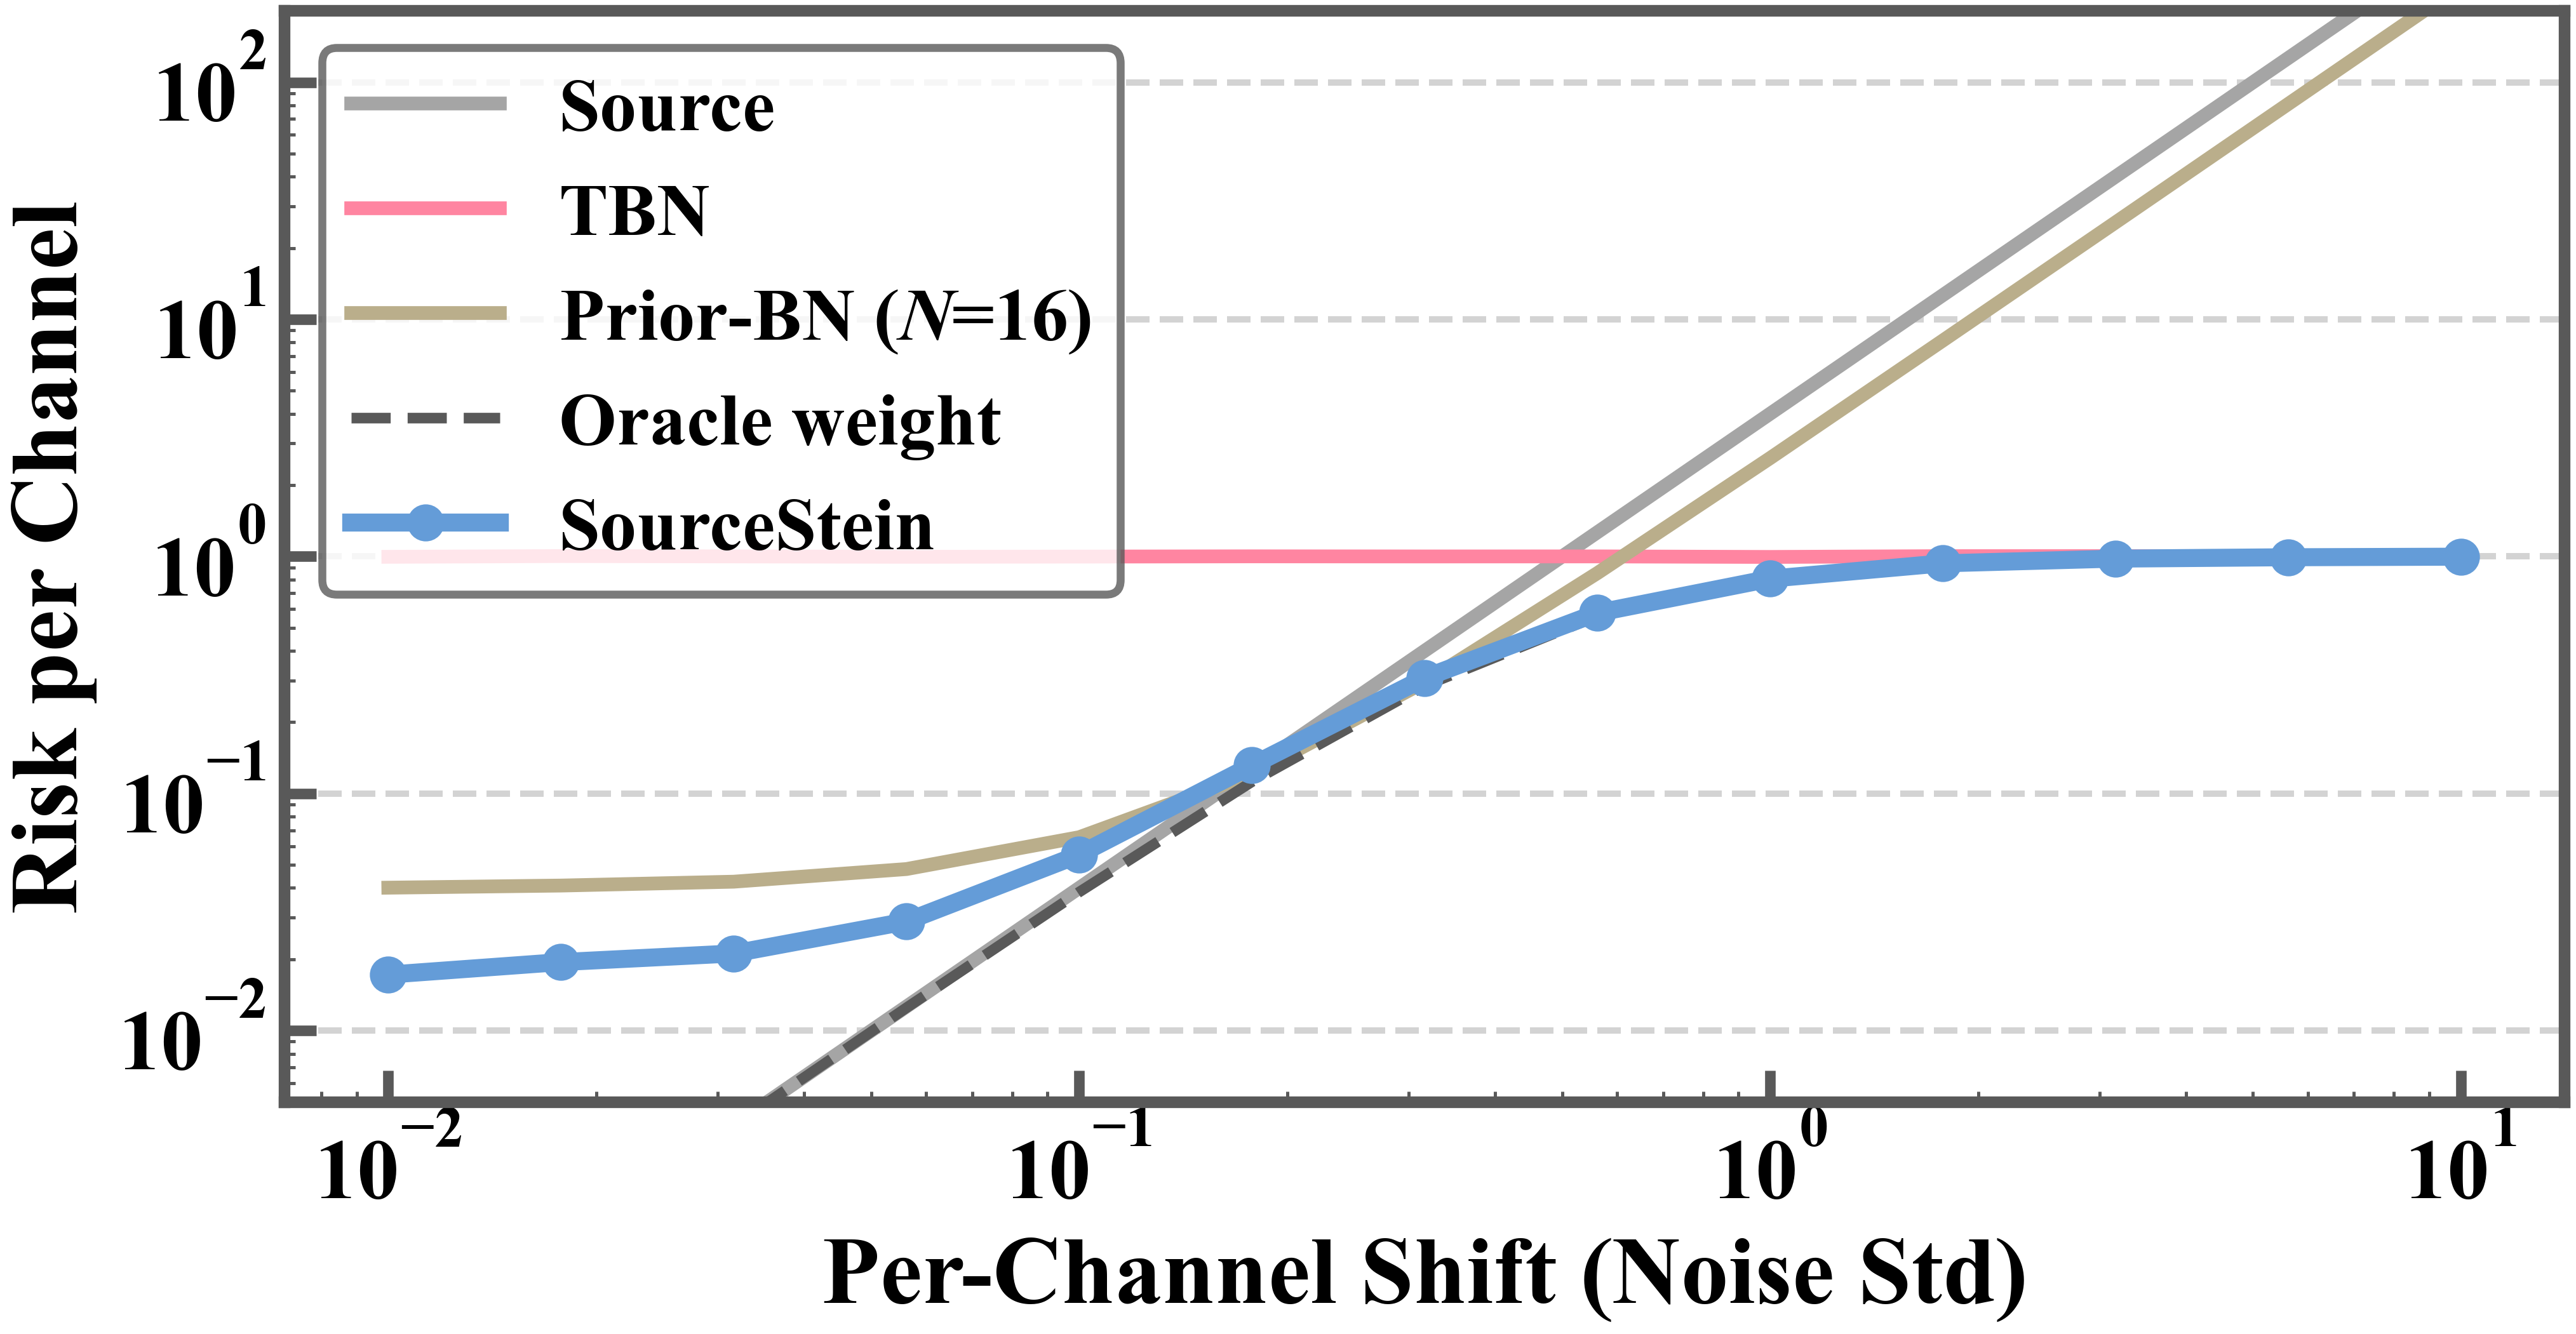
\includegraphics[width=\columnwidth]{figures/exp/synthetic/risk_n4_gauss_s1p0.png}
    \caption{Fixed mixing weights fail at one end of the shift range. Risk of the estimated mean (per channel, in noise units, log scale) for batches of $n{=}4$ simulated samples with $C{=}64$ channels, as the shift increases. Source statistics and Prior-BN incur a shift bias that increases with the shift, while TBN incurs the full estimation variance at each shift; SourceStein follows the oracle weight across the range.}
    \label{fig:teaser-figure}
    \vspace{-12pt}
\end{figure}

Batch normalization (BN) \cite{BatchNorm} is part of most convolutional classifiers.
Each BN layer normalizes its features with statistics collected on the training data, which ties the whole network to the training distribution.
Under \concept{covariate shift} \cite{BN-Adapt}, such as fog or sensor noise at test time, these statistics no longer match the test features.
As a result, the accuracy of a model trained on clean images decreases sharply \cite{CIFAR10-C}.
\concept{Test-time normalization} \cite{AlphaBN} removes much of this loss by re-estimating the BN statistics on the test data, with no labels and no training \cite{PredictionBN, BN-Adapt}.
Because it changes only the statistics, it applies to any trained BN network and adds almost no computation.
While effective, this fix depends on how many test inputs arrive together: streams and edge devices often deliver a handful of images at a time \cite{NOTE, SAR}, and statistics computed from so few samples are unreliable \cite{BN-Adapt}.

To handle small batches, current methods combine two estimates: the stored \concept{source statistics} \cite{BN-Adapt} and the \concept{test batch statistics} \cite{UnMix-TNS}.
In our notation, a layer normalizes with the mean $\boldsymbol{\mu}^{\text{src}} + \lambda(\hat{\boldsymbol{\mu}} - \boldsymbol{\mu}^{\text{src}})$, where $\hat{\boldsymbol{\mu}}$ is the mean of the $n$ test samples and $\lambda \in [0,1]$ is a \concept{mixing weight} (the variance is treated alike).
TBN \cite{PredictionBN} uses $\lambda{=}1$, Prior-BN \cite{BN-Adapt} uses $\lambda{=}n/(n{+}N)$ with a pseudo sample size $N$, and $\alpha$-BN \cite{AlphaBN} uses a constant $\lambda{=}1{-}\alpha$.
Each choice is set by a hyperparameter and the batch size, and works well in the setting it was tuned for.
These rules have made test-time normalization a strong training-free baseline \cite{TENT}.
Whether full, prior-weighted or constant, these rules share one design: the mixing weight is fixed before the test batch is seen.
Consider a batch of four foggy images (the running example of Figure~\ref{fig:main-figure}): Prior-BN assigns it the same weight $4/(4{+}N)$ as a batch of four clean images, although only the foggy batch has moved away from the training data.

Intuitively, effective test-time statistics should be adaptive (\ie follow the shift of the test data) and stable (\ie not fluctuate with the few samples in a batch).
However, a weight fixed in advance cannot be both.
As shown in Figure~\ref{fig:teaser-figure} on simulated features, this design causes two limitations:
\begin{itemize}[leftmargin=*]
    \item \textbf{Stale Source Statistics.} When the shift is large and the weight is small, the mixed mean remains near the source mean. As a result, the normalization inherits a \concept{shift bias} that increases with the square of the shift. This bias affects Prior-BN most at large $N$, whose weight is in fact optimal for only one shift size (see Section~\ref{sec:shrinkage-problem}).
    \item \textbf{Noisy Batch Statistics.} When the batch is small and the weight is large, the mixed mean copies the sampling noise of $\hat{\boldsymbol{\mu}}$. Consequently, the normalization incurs an \concept{estimation variance} that does not decrease with the shift. This variance makes TBN err on most clean inputs at batch size one (see Table~\ref{tab:clean}).
\end{itemize}

To address these issues, we propose \textbf{SourceStein}, an adaptive and stable rule for test-time normalization.
The key idea is to set the mixing weight after the test batch is seen, from the batch itself, by comparing how far the batch has moved with how far it would move by chance.
In this way, the weight becomes a measurement of each batch rather than a setting chosen before deployment.
However, this comparison requires the noise level of the batch statistics, which a single test image cannot provide.
Moreover, a plug-in estimate of the best weight is itself noisy for small batches \cite{Efron-Morris}.
To this end, we equip each BN layer with two parts.
The first is a \textbf{shift score} $S = n\|\hat{\boldsymbol{\mu}} - \boldsymbol{\mu}^{\text{src}}\|^2_{\boldsymbol{\Sigma}^{-1}}$, which whitens the observed shift with between-sample variances $\boldsymbol{\Sigma}$ stored from the training data.
The second is a \textbf{Stein weight} $\hat{\lambda} = (1 - (C{-}2)/S)_+$ over the $C$ channels of the layer, \ie the positive-part \concept{James--Stein estimator} \cite{James-Stein} with the source statistics as its target.
The shift score keeps the statistics adaptive when the test data have moved, while the Stein weight keeps them stable when the move is within the noise.
Under a Gaussian model, this rule never has a higher risk than TBN and remains close to the best fixed weight for the actual shift.

We then run experiments with two networks on CIFAR-10-C \cite{CIFAR10-C} to test SourceStein.
First, SourceStein generally reduces the error of TBN, Prior-BN and $\alpha$-BN for batches of 1 to 16 images and matches them for larger batches (\cf Section~\ref{sec:main-performance}).
Second, its weight increases with the batch size and with the shift, as the analysis predicts (\cf Section~\ref{sec:mechanism}).
Third, adapting the variance and pooling the score over channels both contribute, and no pseudo sample size of Prior-BN matches SourceStein (\cf Section~\ref{sec:ablation-study}).
Fourth, inside entropy minimization the rule helps one of the two networks (\cf Section~\ref{sec:extension}).
Overall, the rule replaces a hyperparameter that previously had to be tuned on labelled shifted data with a decision made from each batch.
We highlight that SourceStein is adaptive and stable at the cost of two stored vectors per layer and no training.

\section{Preliminary}
% Roadmap; 2.1 task; 2.2 base paradigm (mixing rules) ending with the limitation.
Section~\ref{sec:task-formulation} first defines test-time normalization.
After that, Section~\ref{sec:base-paradigm} writes the existing rules as one family of mixed statistics and explains why small batches are hard for them.

\subsection{Task Formulation} \label{sec:task-formulation}
\textbf{Fully test-time adaptation.} We start from a classifier $f$ trained on a source distribution $\mathcal{P}^{\text{src}}$ and deployed on a shifted target distribution $\mathcal{P}^{\text{tgt}}$ \cite{TENT}.
Unlabelled test inputs arrive in batches $\mathcal{B} = \{\mathbf{x}_i\}_{i=1}^{n}$ of a small size $n$, and the model must predict each batch without labels, source data or further training.
We consider the setting in which each batch is drawn independently from $\mathcal{P}^{\text{tgt}}$ and the model keeps no memory across batches, which isolates the effect of the batch size.
This setting matches the evaluation of test-time normalization in prior work \cite{PredictionBN, BN-Adapt}, and it is the hardest one for batch statistics, since no evidence accumulates over time.

\textbf{Batch normalization.} Consider one BN layer with $C$ channels \cite{BatchNorm}.
For a feature map $\mathbf{h} \in \mathbb{R}^{C \times H \times W}$, the layer outputs:
\begin{equation}\label{eq:bn}
\mathrm{BN}(\mathbf{h}) = \boldsymbol{\gamma} \odot \frac{\mathbf{h} - \boldsymbol{\mu}}{\sqrt{\mathbf{v} + \epsilon}} + \boldsymbol{\beta},
\end{equation}
where $\boldsymbol{\gamma}, \boldsymbol{\beta} \in \mathbb{R}^{C}$ are the learned affine parameters, $\boldsymbol{\mu}, \mathbf{v} \in \mathbb{R}^{C}$ are the mean and variance used for normalization (broadcast over the spatial positions), and $\epsilon$ is a small constant.
After training, the layer stores the source statistics $\boldsymbol{\mu}^{\text{src}}$ and $\mathbf{v}^{\text{src}}$ (running averages over the training data), and the standard model uses them for each test input.

\subsection{Mixed Statistics for Test-Time Normalization} \label{sec:base-paradigm}
\textbf{Per-sample and batch statistics.} For test sample $i$, let $\mathbf{m}_i \in \mathbb{R}^{C}$ be the spatial mean of its feature map and $\mathbf{u}_i \in \mathbb{R}^{C}$ the spatial mean of $(\mathbf{h}_i - \boldsymbol{\mu}^{\text{src}})^2$, its second moment about the source mean.
The test batch statistics are then:
\begin{equation}\label{eq:batch-stats}
\begin{aligned}
\hat{\boldsymbol{\mu}} &= \tfrac{1}{n}\textstyle\sum_{i=1}^{n} \mathbf{m}_i, \qquad \hat{\mathbf{u}} = \tfrac{1}{n}\textstyle\sum_{i=1}^{n} \mathbf{u}_i,\\
\hat{\mathbf{v}} &= \hat{\mathbf{u}} - (\hat{\boldsymbol{\mu}} - \boldsymbol{\mu}^{\text{src}})^{2},
\end{aligned}
\end{equation}
where $\hat{\mathbf{v}}$ is the usual batch variance over all $nHW$ positions, written through $\hat{\mathbf{u}}$ so that both statistics are averages of independent per-sample terms.

\textbf{Mixing rules.} Existing test-time normalization methods replace $\boldsymbol{\mu}$ in Equation~\ref{eq:bn} by a convex combination of the two statistics:
\begin{equation}\label{eq:mixing}
\boldsymbol{\mu}(\lambda) = \boldsymbol{\mu}^{\text{src}} + \lambda\,(\hat{\boldsymbol{\mu}} - \boldsymbol{\mu}^{\text{src}}), \qquad \lambda \in [0, 1],
\end{equation}
and treat the variance in the same way.
The source model is $\lambda{=}0$ and TBN \cite{PredictionBN} is $\lambda{=}1$.
Prior-BN \cite{BN-Adapt} reads the source statistics as a prior worth $N$ samples and sets $\lambda = n/(n+N)$, recommending $N \in [8, 128]$ for small batches.
$\alpha$-BN \cite{AlphaBN} mixes the means and standard deviations with a constant $\lambda = 1 - \alpha$, with $\alpha{=}0.9$ for classification.
This weight does not depend on $n$, and $\alpha$-BN keeps most of the source statistics even when a large batch would allow a precise estimate.
Methods that additionally train the affine parameters, such as TENT \cite{TENT}, build on the same statistics.
Other rules set $\lambda$ through a schedule over the test stream \cite{DUA} or learn one weight per layer on augmented source data before deployment \cite{TTN}.
Whether set by a hyperparameter, a schedule or a training phase, the weight is decided before the test batch arrives.

\textbf{Noise of the batch statistics.} The per-sample means $\mathbf{m}_i$ of a batch are independent draws.
As a result, the batch mean $\hat{\boldsymbol{\mu}}$ has covariance $\operatorname{diag}(\boldsymbol{\tau}^2)/n$, where $\boldsymbol{\tau}^2$ collects the between-sample variances of the channel means.
For $n{=}1$, this noise equals the full spread of single images, and TBN normalizes each image by its own statistics, which can remove the global contrast and brightness that the classifier relies on.
The same holds for $\hat{\mathbf{u}}$ with the between-sample variances $\boldsymbol{\rho}^2$ of the second moments.
In contrast, the shift $\boldsymbol{\mu}^{\text{tgt}} - \boldsymbol{\mu}^{\text{src}}$, where $\boldsymbol{\mu}^{\text{tgt}} = \mathbb{E}_{\mathcal{P}^{\text{tgt}}}[\mathbf{m}_i]$ is the target mean, does not depend on $n$.
Therefore, a good weight should compare the two quantities, which the rules above never do.
Each of their weights depends only on $n$ and a hyperparameter chosen in advance.
Still, a rule that cannot tell a batch that has moved far from one that has moved by chance leaves the statistics either stale or noisy, which limits test-time normalization exactly when batches are small.

\section{Methodology}
% Plan (type T): 3.1 objective with two error terms (shift bias / estimation variance) + oracle weight;
% 3.2 adaptive side: whitened shift score (limitation i, Stale Source Statistics);
% 3.3 stable side: Stein weight + lemma + proposition (limitation ii, Noisy Batch Statistics);
% 3.4 assembled SourceStein for means and variances + cost.
In this section, we present \textbf{SourceStein}, an adaptive and stable rule that chooses the mixing weight of Equation~\ref{eq:mixing} separately for each test batch and each BN layer.
We first write the error of the mixed statistics as a sum of a shift bias and an estimation variance in Section~\ref{sec:shrinkage-problem}, which yields the best mixing weight in closed form.
After that, Section~\ref{sec:shift-score} estimates the unknown shift with a whitened shift score.
Then, Section~\ref{sec:stein-weight} turns the score into the Stein weight and states its risk guarantee.
Finally, Section~\ref{sec:sourcestein} applies the same rule to the variances and assembles the complete method.

\begin{figure*}[t]
    \centering
    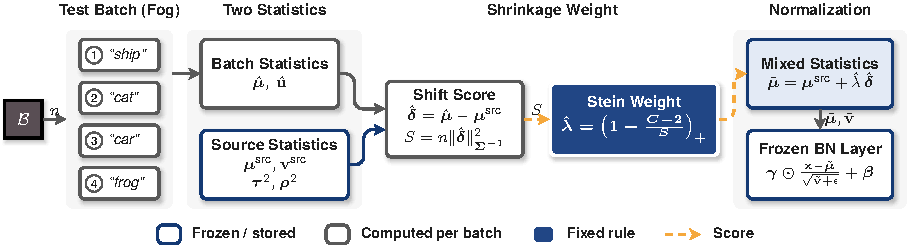
\includegraphics{figures/framework/main_figure.pdf}
    \caption{Overview of SourceStein at one BN layer. A test batch of $n$ fog-corrupted images yields the batch statistics $\hat{\boldsymbol{\mu}}, \hat{\mathbf{u}}$, while the frozen layer stores the source statistics $\boldsymbol{\mu}^{\text{src}}, \mathbf{v}^{\text{src}}$ and the between-sample variances $\boldsymbol{\tau}^2, \boldsymbol{\rho}^2$ measured once on training data. (1) The shift score $S$ measures the observed shift $\hat{\boldsymbol{\delta}}$ in units of the noise expected from $n$ samples. (2) The Stein weight $\hat{\lambda}$ keeps only the part of the shift that exceeds this noise. (3) The mixed statistics replace the stored ones inside the unchanged BN layer.}
    \label{fig:main-figure}
    \vspace{-6pt}
\end{figure*}

\subsection{Test-Time Statistics as a Shrinkage Problem} \label{sec:shrinkage-problem}
To choose $\lambda$ for a given batch, we first state what a good mixed mean should achieve.
Recall that $\boldsymbol{\mu}^{\text{tgt}}$ is the mean the layer would use with unlimited test data, and let $\boldsymbol{\delta} = \boldsymbol{\mu}^{\text{tgt}} - \boldsymbol{\mu}^{\text{src}}$ be the true shift and $\boldsymbol{\Sigma} = \operatorname{diag}(\boldsymbol{\tau}^2)$ the covariance of a single per-sample mean $\mathbf{m}_i$.
The batch mean $\hat{\boldsymbol{\mu}}$ then has covariance $\boldsymbol{\Sigma}/n$.
We measure the error of Equation~\ref{eq:mixing} in the noise units of the layer:
\begin{equation}\label{eq:risk}
\begin{aligned}
R(\lambda) &= \mathbb{E}\, n \big\|\boldsymbol{\mu}(\lambda) - \boldsymbol{\mu}^{\text{tgt}}\big\|^{2}_{\boldsymbol{\Sigma}^{-1}}\\
&= \underbrace{(1-\lambda)^{2}\,\Delta}_{\text{shift bias}} + \underbrace{\lambda^{2}\,C}_{\text{estimation variance}},
\end{aligned}
\end{equation}
where $\|\mathbf{x}\|^2_{\boldsymbol{\Sigma}^{-1}} = \mathbf{x}^{\top}\boldsymbol{\Sigma}^{-1}\mathbf{x}$ and $\Delta = n\|\boldsymbol{\delta}\|^2_{\boldsymbol{\Sigma}^{-1}}$ is the whitened shift.
Specifically, the first term is the shift bias of keeping the source statistics, and the second is the estimation variance of trusting $n$ samples.
Setting the derivative to zero yields the best weight of the family:
\begin{equation}\label{eq:oracle}
\lambda^{\star} = \frac{\Delta}{\Delta + C}, \qquad R(\lambda^{\star}) = \frac{C\,\Delta}{\Delta + C}.
\end{equation}
This oracle weight moves toward the batch as the shift or the batch increases, and remains near the source when the shift is small compared with the noise.
In contrast, the weight $n/(n+N)$ of Prior-BN equals $\lambda^{\star}$ only when $\|\boldsymbol{\delta}\|^2_{\boldsymbol{\Sigma}^{-1}} = C/N$, \ie for one shift size per pseudo sample size.
TBN incurs $R(1) = C$ at each shift, and the source model incurs $R(0) = \Delta$, which is unbounded in the shift.

\subsection{Adaptive Mixing via a Whitened Shift Score} \label{sec:shift-score}
To counter stale source statistics, the weight must respond to the shift $\Delta$, which is unknown at test time.
We estimate it from the test batch statistics through the observed shift $\hat{\boldsymbol{\delta}} = \hat{\boldsymbol{\mu}} - \boldsymbol{\mu}^{\text{src}}$ through the shift score:
\begin{equation}\label{eq:shift-score}
S = n\,\big\|\hat{\boldsymbol{\delta}}\big\|^{2}_{\boldsymbol{\Sigma}^{-1}} = n \sum_{c=1}^{C} \frac{(\hat{\mu}_c - \mu^{\text{src}}_c)^{2}}{\tau^{2}_c},
\end{equation}
whose expectation is $\mathbb{E}[S] = \Delta + C$: the true shift plus the noise of $n$ samples.
Specifically, the score requires the noise level $\boldsymbol{\tau}^2$, which a batch of one image cannot estimate.
Therefore, we measure it once on the training data, as the variance of the per-sample means $\mathbf{m}_i$ over $5{,}000$ training images, and store it together with $\boldsymbol{\mu}^{\text{src}}$.
Under this choice, a shift that is large compared with the training spread of single images drives $S$ far above $C$, and the weight can follow it.
In contrast, a clean batch has $\mathbb{E}[S] = C$ up to the train--test gap of the source statistics, and its score remains close to the number of channels.

\textbf{Choice of the noise level.} The source noise level is an assumption: a corruption can change the spread of single images as well as their mean.
We keep it because it is available for each batch size, including $n{=}1$, while a noise level estimated from $n$ test samples is itself a noisy ratio for small $n$.
Section~\ref{sec:ablation-study} compares both choices, and Appendix~\ref{apdx:synthetic} shows what a misestimated noise level costs in simulation.

\subsection{Stable Mixing with the Stein Weight} \label{sec:stein-weight}
With the shift measured by $S$, the plug-in of Equation~\ref{eq:oracle} would be $1 - C/S$.
However, $S$ is noisy when $n$ is small, and a plug-in weight inherits this noise exactly where the estimation variance matters most.
Therefore, we rely on the following classical result, in which the shrinkage target is the source mean:
\begin{lemma}[James--Stein Estimator \cite{James-Stein}]\label{lemma:james-stein}
Let $\mathbf{z} \sim \mathcal{N}(\boldsymbol{\theta}, \mathbf{I}_C)$ with $C \ge 3$, let $\mathbf{a} \in \mathbb{R}^{C}$ be fixed, and let $s = \|\mathbf{z} - \mathbf{a}\|^2$. Then $\hat{\boldsymbol{\theta}} = \mathbf{a} + (1 - (C-2)/s)(\mathbf{z} - \mathbf{a})$ has risk $\mathbb{E}\|\hat{\boldsymbol{\theta}} - \boldsymbol{\theta}\|^2 = C - (C-2)^2\,\mathbb{E}[1/s]$, and clipping the factor at zero does not increase the risk \cite{Efron-Morris}.
\end{lemma}
Applying the lemma to the whitened batch mean $\mathbf{z} = \sqrt{n}\,\boldsymbol{\Sigma}^{-1/2}\hat{\boldsymbol{\mu}}$ with $\mathbf{a} = \sqrt{n}\,\boldsymbol{\Sigma}^{-1/2}\boldsymbol{\mu}^{\text{src}}$, for which $s = S$, yields the Stein weight:
\begin{equation}\label{eq:stein-weight}
\hat{\lambda} = \Big(1 - \frac{C-2}{S}\Big)_{+},
\end{equation}
where $(x)_+ = \max(x, 0)$.
As a result, the weight is zero until the shift score exceeds $C-2$ and approaches one as the shift dominates the noise.

\textbf{One weight per layer.} The $C$ channels of a layer share one weight, because the lemma pools their evidence: a shift that is small in each channel but present in many of them still increases $S$.
In contrast, a separate weight per channel would base each decision on a single noisy value, and the guarantee below requires $C \ge 3$.
However, the price is that channels with different shifts receive the same weight, which Section~\ref{sec:ablation-study} examines.
The risk of the Stein weight compares with the two fixed extremes and with the oracle as follows:
\begin{proposition}\label{prop:risk}
Assume $\hat{\boldsymbol{\mu}} \sim \mathcal{N}(\boldsymbol{\mu}^{\text{tgt}}, \boldsymbol{\Sigma}/n)$ with $C \ge 3$. Then the Stein weight satisfies $R(\hat{\lambda}) \le C - (C-2)^2/(C + \Delta)$, which is \textbf{below the risk $C$ of TBN} for each shift, and $R(\hat{\lambda}) - R(\lambda^{\star}) \le 4(C-1)/(C+\Delta) < 4$.
\end{proposition}
Specifically, the first bound follows from Lemma~\ref{lemma:james-stein} and Jensen's inequality $\mathbb{E}[1/S] \ge 1/\mathbb{E}[S]$, and the second subtracts Equation~\ref{eq:oracle} (see Appendix~\ref{apdx:proof} for the proof).
Measured per channel, the excess over the oracle is below $4/C$, which is small for layers with 16 to 128 channels.

\textbf{Relation to Prior-BN.} Each Stein weight corresponds to a pseudo sample size $\hat{N} = n(1-\hat{\lambda})/\hat{\lambda}$ of Prior-BN, chosen per layer and per batch.
Specifically, a batch whose shift score is close to $C$ receives a very large $\hat{N}$ and keeps the source statistics, while a batch with a large score receives a small $\hat{N}$ and moves toward its own statistics.
Prior-BN, in contrast, uses one $N$ for all layers, batches and corruptions.

\textbf{Discussion.} The Stein weight has an empirical Bayes reading \cite{Efron-Morris}: $(C-2)/S$ estimates the share of the observed shift that is noise, and $\hat{\lambda}$ keeps the rest.
Moreover, the choice of the shrinkage target matters here.
Prior uses of Stein shrinkage in normalization layers shrink toward a centre computed from the same batch during training \cite{JS-Norm, Stein-BN-Adv}, which reduces noise but cannot correct a shift.
SourceStein instead shrinks toward the source statistics, so that the target contains the knowledge of the training data and the batch only has to supply the evidence of a shift.

\begin{algorithm}[t]
  \captionsetup{labelformat=default,labelsep=colon,name=Algorithm}
  \caption{Normalization with SourceStein}
  \label{alg:sourcestein}
\begin{algorithmic}
  \STATE {\bfseries Input:} test features $\{\mathbf{h}_i\}_{i=1}^{n}$ at one BN layer; stored $\boldsymbol{\mu}^{\text{src}}, \mathbf{v}^{\text{src}}, \boldsymbol{\tau}^2, \boldsymbol{\rho}^2, \boldsymbol{\gamma}, \boldsymbol{\beta}$.
  \STATE \CommentBelow{batch statistics (Equation~\ref{eq:batch-stats})}
  \STATE $\mathbf{m}_i \leftarrow \operatorname{mean}_{hw}\mathbf{h}_i$, \ $\mathbf{u}_i \leftarrow \operatorname{mean}_{hw}(\mathbf{h}_i - \boldsymbol{\mu}^{\text{src}})^2$
  \STATE $\hat{\boldsymbol{\mu}} \leftarrow \operatorname{mean}_i \mathbf{m}_i$, \ $\hat{\mathbf{u}} \leftarrow \operatorname{mean}_i \mathbf{u}_i$
  \STATE \tikzmk{algA}\CommentBelow{shift scores and Stein weights}
  \STATE $S_\mu \leftarrow n\sum_c (\hat{\mu}_c - \mu^{\text{src}}_c)^2/\tau^2_c$
  \STATE $S_u \leftarrow n\sum_c (\hat{u}_c - v^{\text{src}}_c)^2/\rho^2_c$
  \STATE $\hat{\lambda}_\mu \leftarrow (1 - \frac{C-2}{S_\mu})_+$, \ $\hat{\lambda}_u \leftarrow (1 - \frac{C-2}{S_u})_+$\tikzmk{algB}
  \STATE \CommentBelow{mixed statistics (Equation~\ref{eq:sourcestein})}
  \STATE $\tilde{\boldsymbol{\mu}} \leftarrow \boldsymbol{\mu}^{\text{src}} + \hat{\lambda}_\mu(\hat{\boldsymbol{\mu}} - \boldsymbol{\mu}^{\text{src}})$
  \STATE $\tilde{\mathbf{u}} \leftarrow \mathbf{v}^{\text{src}} + \hat{\lambda}_u(\hat{\mathbf{u}} - \mathbf{v}^{\text{src}})$
  \STATE $\tilde{\mathbf{v}} \leftarrow \max(\tilde{\mathbf{u}} - (\tilde{\boldsymbol{\mu}} - \boldsymbol{\mu}^{\text{src}})^2, 10^{-5})$
  \STATE {\bfseries return} $\boldsymbol{\gamma} \odot (\mathbf{h}_i - \tilde{\boldsymbol{\mu}})/\sqrt{\tilde{\mathbf{v}} + \epsilon} + \boldsymbol{\beta}$ for each $i$.
\end{algorithmic}
\boxit[Stein]{PhaseABg}{algA}{algB}
\end{algorithm}

\subsection{SourceStein} \label{sec:sourcestein}
Combining the shift score with the Stein weight, SourceStein treats the variance in the same way as the mean.
The per-sample second moments $\mathbf{u}_i$ have mean $\mathbf{v}^{\text{src}}$ on source data and between-sample variances $\boldsymbol{\rho}^2$, which we store with $\boldsymbol{\tau}^2$.
For each BN layer and each test batch, SourceStein computes:
\begin{equation}\label{eq:sourcestein}
\begin{aligned}
\tilde{\boldsymbol{\mu}} &= \boldsymbol{\mu}^{\text{src}} + \hat{\lambda}_{\mu}\,(\hat{\boldsymbol{\mu}} - \boldsymbol{\mu}^{\text{src}}),\\
\tilde{\mathbf{u}} &= \mathbf{v}^{\text{src}} + \hat{\lambda}_{u}\,(\hat{\mathbf{u}} - \mathbf{v}^{\text{src}}),\\
\tilde{\mathbf{v}} &= \max\!\big(\tilde{\mathbf{u}} - (\tilde{\boldsymbol{\mu}} - \boldsymbol{\mu}^{\text{src}})^{2},\ 10^{-5}\big),
\end{aligned}
\end{equation}
where $\hat{\lambda}_{\mu}$ is Equation~\ref{eq:stein-weight} with $(\hat{\boldsymbol{\mu}}, \boldsymbol{\mu}^{\text{src}}, \boldsymbol{\tau}^2)$ and $\hat{\lambda}_{u}$ is the same rule with $(\hat{\mathbf{u}}, \mathbf{v}^{\text{src}}, \boldsymbol{\rho}^2)$.
The layer then normalizes with $\tilde{\boldsymbol{\mu}}$ and $\tilde{\mathbf{v}}$ in Equation~\ref{eq:bn}, and the next layer sees the adapted features.
When both weights are one, Equation~\ref{eq:sourcestein} is equivalent to the batch statistics of Equation~\ref{eq:batch-stats}; when both are zero, it is equivalent to the source model.
Algorithm~\ref{alg:sourcestein} lists all steps of SourceStein for one layer.

\textbf{Cost.} SourceStein requires one pass over $5{,}000$ unlabelled training images to store $\boldsymbol{\tau}^2$ and $\boldsymbol{\rho}^2$, and no labels, gradients or hyperparameters.
At test time it adds $O(nCHW)$ operations per layer, the same order as computing the batch statistics; further implementation details are in Appendix~\ref{apdx:impl-details}.

\section{Experiments}
% RQ plan: RQ1 performance (Table 1, Table 2) | RQ2 mechanism (Figure 3: weights; synthetic risk in Fig 1 + appendix)
% | RQ3 ablation (Table 3, Figure 4) | RQ4 extension to entropy minimization (Table 4).
In this section, we examine SourceStein through the research questions below:
\begin{itemize}[leftmargin=*]
    \item \textbf{RQ1:} (Performance) Does SourceStein reduce the corruption error of existing mixing rules across batch sizes, and does it keep the error on clean data?
    \item \textbf{RQ2:} (Mechanism) How does the Stein weight balance the shift bias and the estimation variance as the batch size and the shift change?
    \item \textbf{RQ3:} (Ablation Study) What do pooling, variance shrinkage and the source noise level contribute, and can any fixed pseudo sample size match SourceStein?
    \item \textbf{RQ4:} (Extension) Can SourceStein replace the batch statistics inside entropy minimization?
\end{itemize}

\textbf{Models.} We train two BN networks from scratch on the CIFAR-10 training set on CPU: CNN-8, a VGG-style network \cite{VGG} with six convolution and BN layers ($86.54\%$ clean test accuracy), and ResNet-14, a residual network \cite{ResNet} with fifteen BN layers ($82.56\%$).
Both use standard augmentation and SGD; Appendix~\ref{apdx:impl-details} reports the training recipe.

\textbf{Evaluation.} We test on CIFAR-10-C \cite{CIFAR10-C}, which applies 15 common corruptions to the CIFAR-10 test set, at the highest severity 5 (severity 3 is reported in Appendix~\ref{apdx:experiments}).
For each corruption, we draw a fixed random subset of $1{,}000$ test images, shuffle it into batches of size $n \in \{1, 2, 4, 8, 16, 64, 200\}$, and report the top-1 error averaged over the 15 corruptions.
All methods see the same images in the same order, and the statistics are recomputed for each batch without memory across batches.

\textbf{Baselines.} We compare with four rules of Equation~\ref{eq:mixing}: the Source model, TBN \cite{PredictionBN}, Prior-BN \cite{BN-Adapt} with the pseudo sample size $N{=}16$, and $\alpha$-BN \cite{AlphaBN} with $\alpha{=}0.9$, as recommended by their authors.
As a privileged reference, Oracle-$N$ picks the best $N \in \{2, 4, \ldots, 256\}$ of Prior-BN for each network and batch size on the test results themselves.
All methods share the trained weights, and differences come from the normalization statistics alone.

% Main table: table* (prints atop the next page); T2-style per-backbone blocks, our row tinted blue.
\begin{table*}[t]
\centering
\renewcommand{\arraystretch}{0.9}
\caption{Error (\%) on CIFAR-10-C at severity 5, averaged over 15 corruptions, for test batches of $n$ images. The best result in each column of a block is \textbf{bold}; the grey Oracle-$N$ row tunes Prior-BN on the test results and is not ranked.}
\label{tab:main-table}
\shrinktofit{0.93\linewidth}{%
\begin{tabular}{cl|ccccccc}
\toprule
\multicolumn{2}{c|}{} & \multicolumn{7}{c}{\textbf{Test Batch Size $n$}} \\
\textbf{Network} & \textbf{Method} & \textbf{1} & \textbf{2} & \textbf{4} & \textbf{8} & \textbf{16} & \textbf{64} & \textbf{200} \\
\midrule
\multirow{6}{*}{ResNet-14}
 & Source & 52.06 & 52.06 & 52.06 & 52.06 & 52.06 & 52.06 & 52.06 \\
 & TBN \cite{PredictionBN} & 89.19 & 55.06 & 44.45 & 37.80 & 33.99 & 31.06 & 30.40 \\
 & Prior-BN \cite{BN-Adapt} & 48.57 & 43.67 & 38.71 & 35.26 & 32.97 & 31.01 & \textbf{30.37} \\
 & $\alpha$-BN \cite{AlphaBN} & 45.89 & 43.95 & 43.06 & 42.33 & 41.96 & 41.74 & 41.67 \\
 & \ablation{Oracle-$N$ (privileged)} & \ablation{43.53} & \ablation{40.65} & \ablation{37.52} & \ablation{35.26} & \ablation{32.97} & \ablation{30.85} & \ablation{30.21} \\
 & \cellcolor{oursrowblue}\textbf{SourceStein (Ours)} & \cellcolor{oursrowblue}\textbf{45.34} & \cellcolor{oursrowblue}\textbf{39.71} & \cellcolor{oursrowblue}\textbf{36.23} & \cellcolor{oursrowblue}\textbf{33.99} & \cellcolor{oursrowblue}\textbf{32.50} & \cellcolor{oursrowblue}\textbf{31.00} & \cellcolor{oursrowblue}30.41 \\
\midrule\midrule
\multirow{6}{*}{CNN-8}
 & Source & 50.01 & 50.01 & 50.01 & 50.01 & 50.01 & 50.01 & 50.01 \\
 & TBN \cite{PredictionBN} & 89.81 & 53.09 & 41.33 & 34.47 & 31.03 & \textbf{28.01} & \textbf{27.25} \\
 & Prior-BN \cite{BN-Adapt} & 47.21 & 43.84 & 39.18 & 34.44 & 31.11 & 28.51 & 27.55 \\
 & $\alpha$-BN \cite{AlphaBN} & 45.61 & 43.99 & 43.21 & 42.63 & 42.63 & 42.28 & 42.11 \\
 & \ablation{Oracle-$N$ (privileged)} & \ablation{43.53} & \ablation{39.42} & \ablation{35.81} & \ablation{32.87} & \ablation{30.80} & \ablation{28.04} & \ablation{27.29} \\
 & \cellcolor{oursrowblue}\textbf{SourceStein (Ours)} & \cellcolor{oursrowblue}\textbf{43.93} & \cellcolor{oursrowblue}\textbf{37.89} & \cellcolor{oursrowblue}\textbf{34.65} & \cellcolor{oursrowblue}\textbf{32.23} & \cellcolor{oursrowblue}\textbf{30.43} & \cellcolor{oursrowblue}28.32 & \cellcolor{oursrowblue}27.41 \\
\bottomrule
\end{tabular}}
\vspace{-12pt}
\end{table*}

\subsection{(RQ1) Error Across Batch Sizes} \label{sec:main-performance}
\begin{figure}[t]
    \centering
    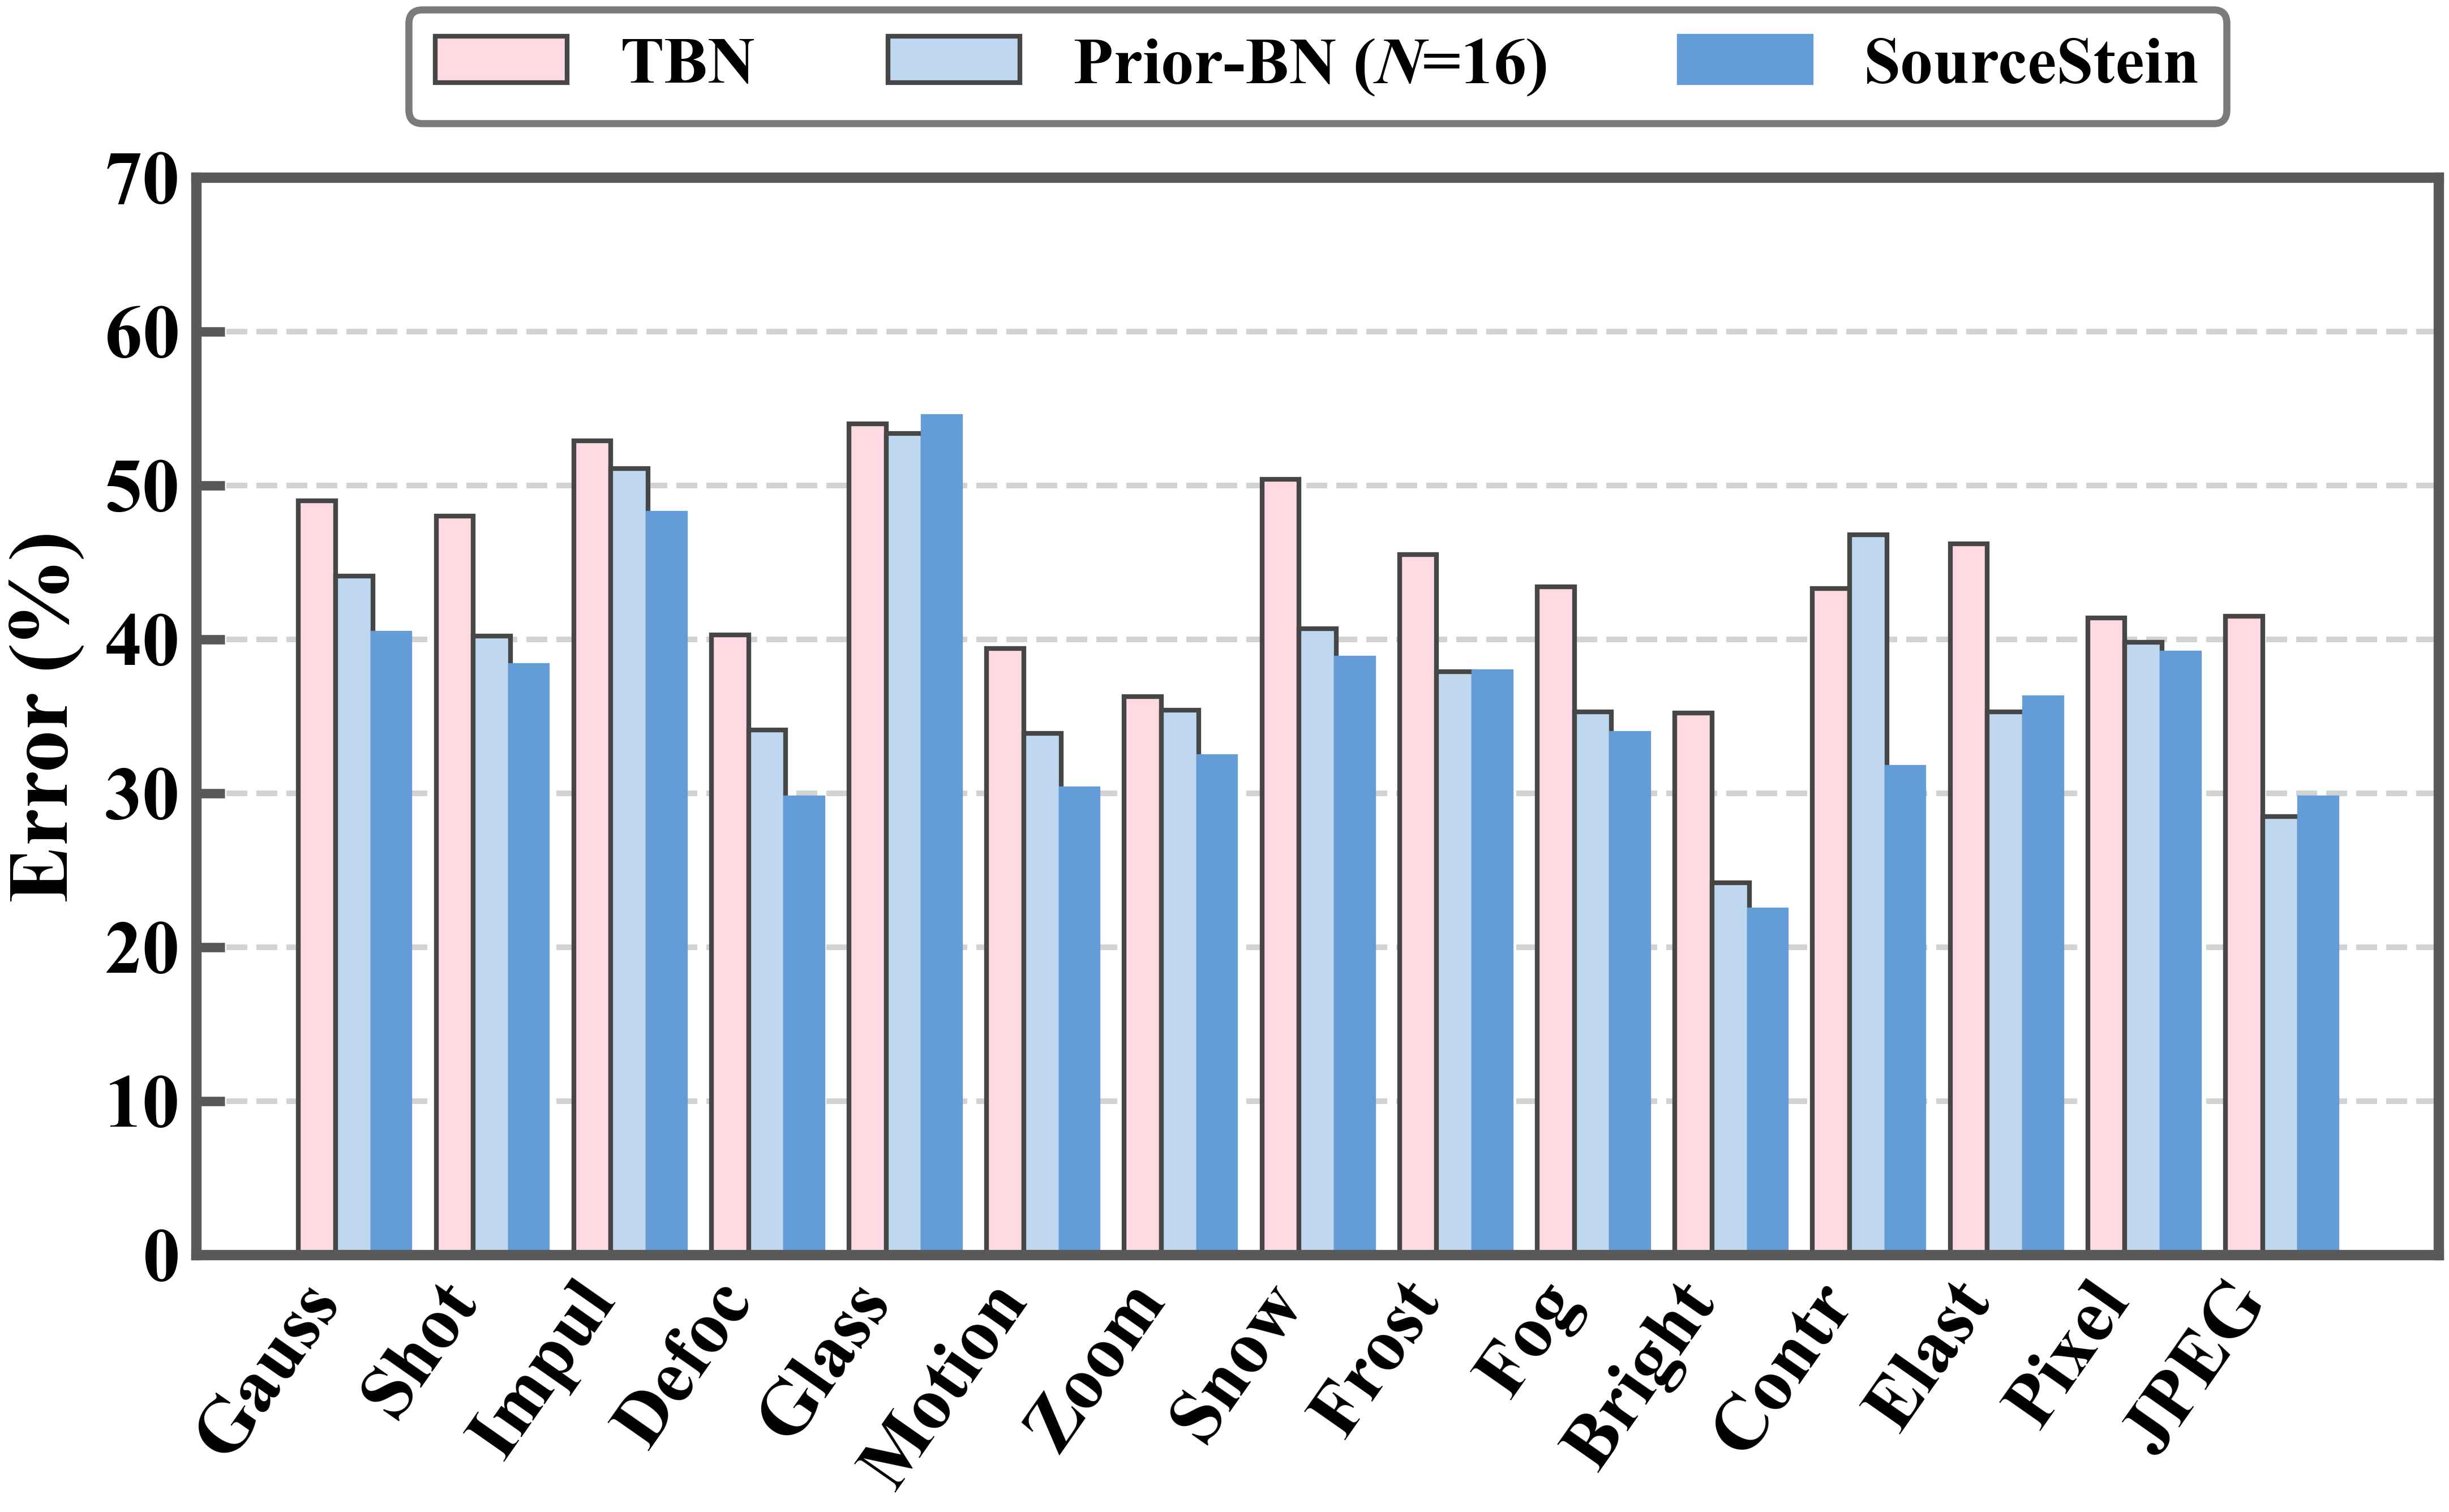
\includegraphics[width=\columnwidth]{figures/exp/mechanism/per_corruption_n4_resnet14.png}
    \caption{Error per corruption on CIFAR-10-C at severity 5 for ResNet-14 and batches of $n{=}4$ images. SourceStein is lowest on 12 of the 15 corruptions, with the largest gain on contrast.}
    \label{fig:per-corruption}
    \vspace{-12pt}
\end{figure}

Table~\ref{tab:main-table} reports the corruption error of each rule, Figure~\ref{fig:error-vs-bs} shows it as a function of the batch size, and Table~\ref{tab:clean} reports the error on clean test images; Appendix~\ref{apdx:experiments} reports the per-corruption results.
We have the following observations:
\begin{itemize}[leftmargin=*]
    \item \textbf{SourceStein has the lowest error for batches of 1 to 16 images.}
    As shown in Table~\ref{tab:main-table}, SourceStein reduces the error of the best unprivileged baseline at each $n \le 16$ on both networks.
    The largest reductions are 3.96 points on ResNet-14 and 5.95 points on CNN-8, both at $n{=}2$.
    Moreover, it is below the privileged Oracle-$N$ for $n$ from 2 to 16, although Oracle-$N$ tunes one pseudo sample size per batch size on the test results.
    We attribute this gain to the mixing weight of SourceStein, which differs per layer and per batch, while any $N$ fixes one weight for all of them.
    At $n{=}1$, Oracle-$N$ remains lower, by 1.81 and 0.40 points.
    Additionally, the gain is spread over most corruptions: as shown in Figure~\ref{fig:per-corruption}, SourceStein is lowest on 12 of 15 corruptions at $n{=}4$ and is above Prior-BN mainly on glass blur, elastic transform and JPEG.
    \item \textbf{For large batches, the rules converge.}
    At $n \ge 64$, SourceStein, TBN and Prior-BN are within 0.5 points of each other, with TBN slightly lower on CNN-8.
    This is expected, since the estimation variance vanishes as $n$ increases and each reasonable weight approaches one.
    In contrast, $\alpha$-BN keeps $90\%$ of the source statistics at each $n$ and remains above $41\%$ error.
\end{itemize}

\begin{table}[t]
\centering
\renewcommand{\arraystretch}{0.9}
\caption{Error (\%) on 1,000 clean CIFAR-10 test images. The best result in each column is \textbf{bold}.}
\label{tab:clean}
\shrinktofit{\columnwidth}{%
\begin{tabular}{l|ccc|ccc}
\toprule
 & \multicolumn{3}{c|}{\textbf{ResNet-14}} & \multicolumn{3}{c}{\textbf{CNN-8}} \\
\textbf{Method} & $n{=}1$ & $n{=}4$ & $n{=}16$ & $n{=}1$ & $n{=}4$ & $n{=}16$ \\
\midrule
Source & \textbf{17.1} & \textbf{17.1} & \textbf{17.1} & 13.9 & 13.9 & 13.9 \\
TBN & 88.5 & 32.4 & 22.8 & 89.9 & 29.7 & 17.8 \\
Prior-BN & 17.7 & 19.7 & 20.3 & \textbf{13.6} & 15.0 & 15.3 \\
$\alpha$-BN & 18.2 & 17.8 & 18.1 & 14.3 & \textbf{13.8} & \textbf{13.9} \\
\rowcolor{oursrowblue} SourceStein & 19.3 & 18.4 & 18.3 & 15.0 & 14.5 & 14.0 \\
\bottomrule
\end{tabular}}
\vspace{-10pt}
\end{table}

\begin{figure}[t]
    \centering
    \begin{subfigure}[t]{\columnwidth}
        \centering
        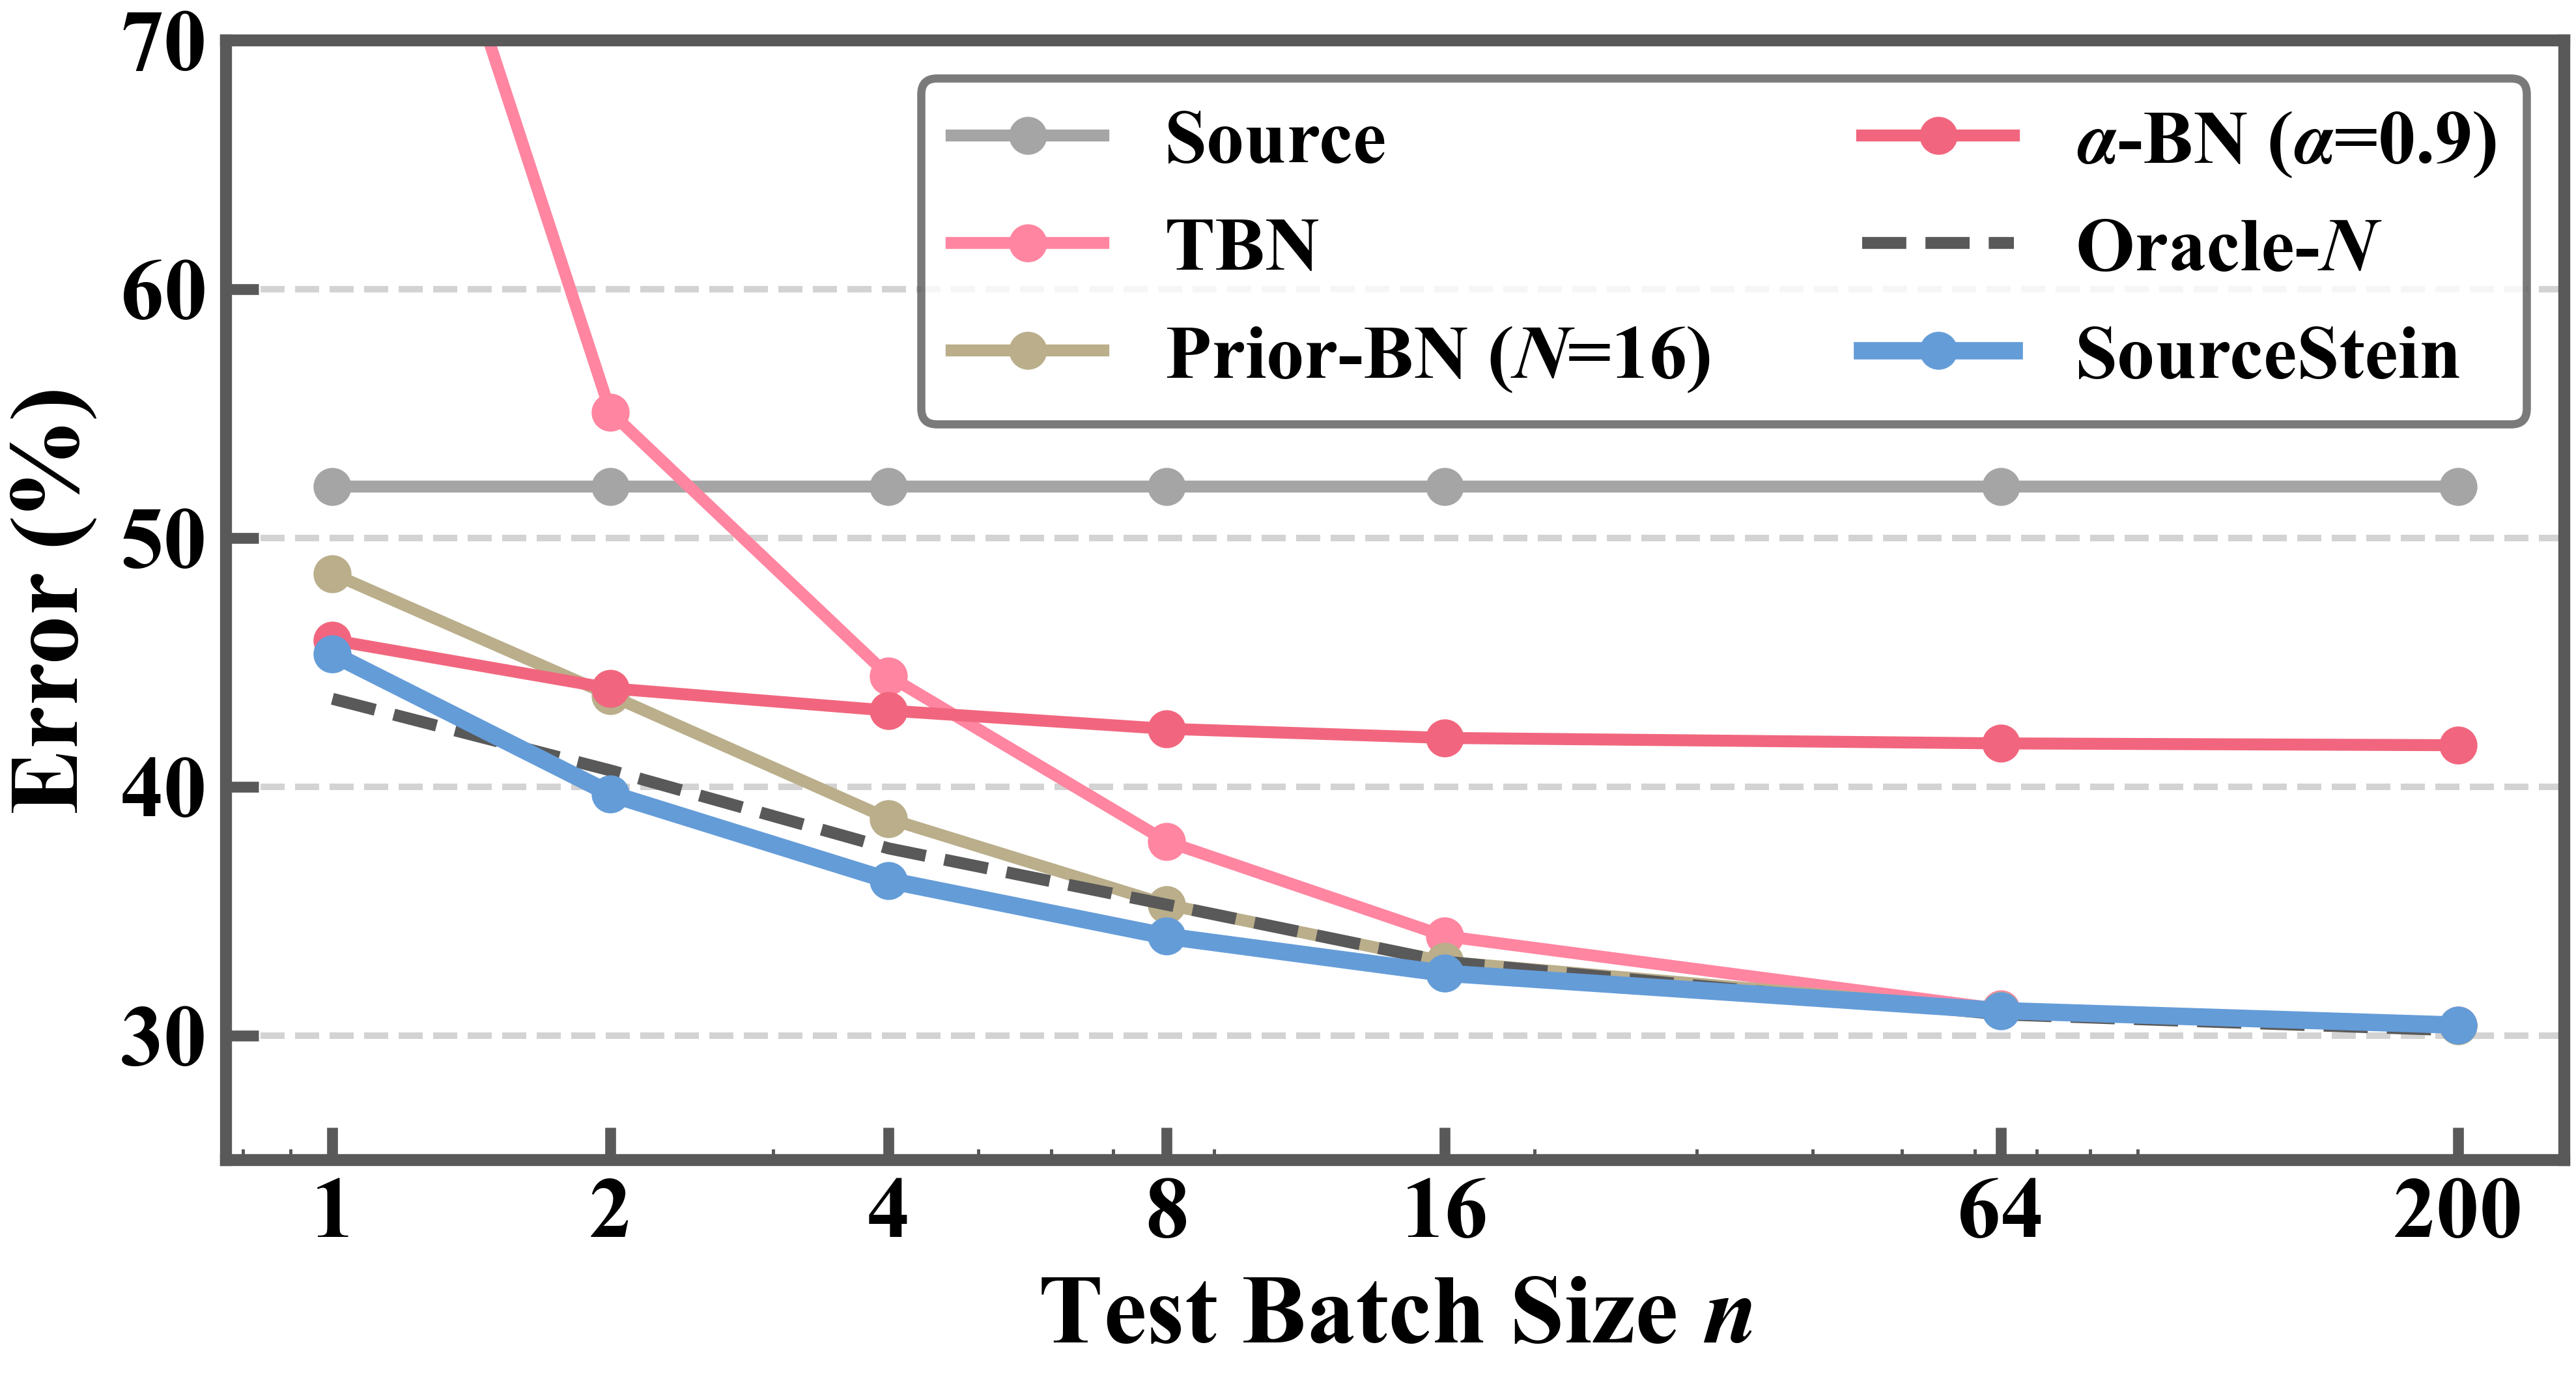
\includegraphics[width=\linewidth]{figures/exp/mechanism/error_vs_bs_resnet14.png}
        \caption{ResNet-14.}
        \label{fig:error-vs-bs-a}
    \end{subfigure}
    \begin{subfigure}[t]{\columnwidth}
        \centering
        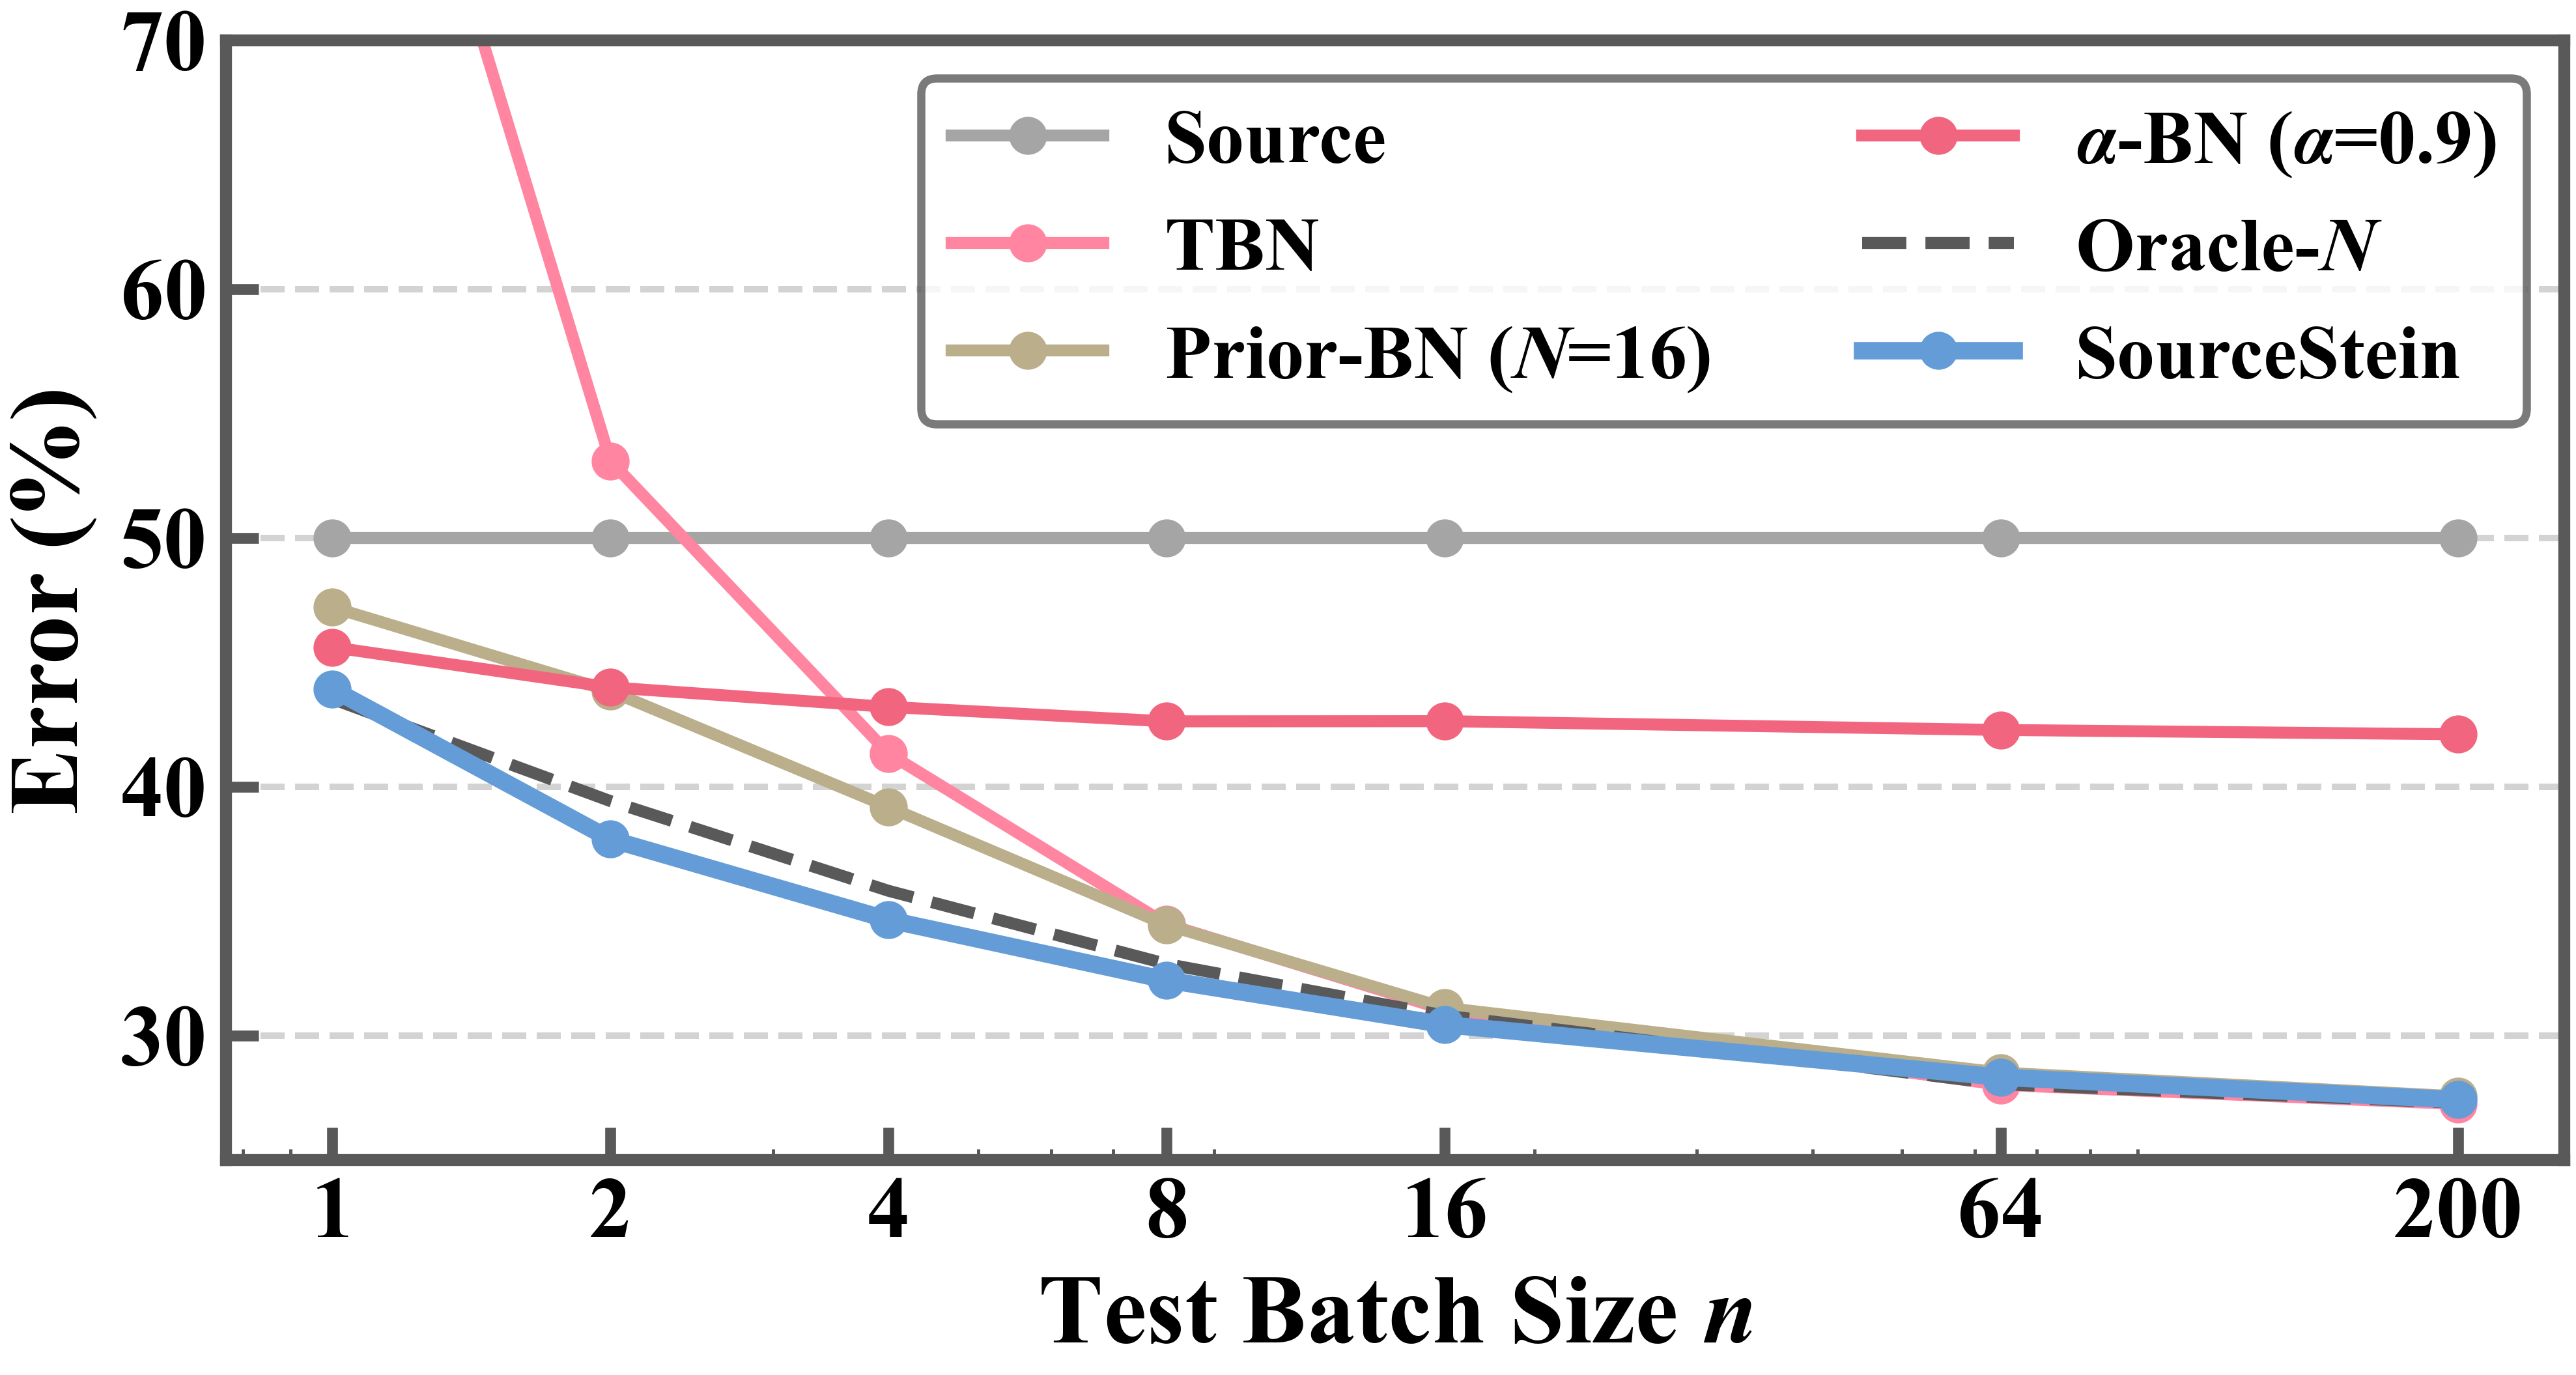
\includegraphics[width=\linewidth]{figures/exp/mechanism/error_vs_bs_cnn8.png}
        \caption{CNN-8.}
        \label{fig:error-vs-bs-b}
    \end{subfigure}
    \caption{Error on CIFAR-10-C at severity 5 as the test batch size increases (log scale). SourceStein is the lowest unprivileged rule up to $n{=}16$ on both networks and joins TBN and Prior-BN for large batches.}
    \label{fig:error-vs-bs}
    \vspace{-12pt}
\end{figure}

\textbf{SourceStein remains close to the source model on clean data.}
Without a shift, any move toward the batch only adds estimation variance.
As shown in Table~\ref{tab:clean}, SourceStein remains within 2.2 points of the Source error at each batch size, while TBN loses up to 76 points and Prior-BN up to 3.7 points.
Such results show that the Stein weight is stable when there is nothing to adapt to, at a small cost compared with $\alpha$-BN, whose fixed weight favours clean data.

\textbf{SourceStein adds little inference time.}
As shown in Table~\ref{tab:time}, SourceStein costs at most 0.42 ms more per image than TBN, at $n{=}1$ on ResNet-14, and is within the timing noise of TBN for larger batches.
This additional work consists of two weighted sums over the channels of each layer, which is small compared with the convolutions.

\begin{table}[t]
\centering
\renewcommand{\arraystretch}{0.9}
\caption{Inference time (ms per image) on one CPU thread for fog images at severity 5, averaged over three passes over 400 images.}
\label{tab:time}
\shrinktofit{\columnwidth}{%
\begin{tabular}{l|ccc|ccc}
\toprule
 & \multicolumn{3}{c|}{\textbf{ResNet-14}} & \multicolumn{3}{c}{\textbf{CNN-8}} \\
\textbf{Method} & $n{=}1$ & $n{=}16$ & $n{=}200$ & $n{=}1$ & $n{=}16$ & $n{=}200$ \\
\midrule
Source & 0.76 & 0.65 & 0.85 & 0.55 & 0.86 & 0.88 \\
TBN & 1.06 & 0.73 & 0.90 & 0.68 & 0.85 & 0.95 \\
Prior-BN & 1.10 & 0.73 & 0.89 & 0.69 & 0.94 & 0.92 \\
\rowcolor{oursrowblue} SourceStein & 1.48 & 0.78 & 0.88 & 0.85 & 0.83 & 0.95 \\
\bottomrule
\end{tabular}}
\vspace{-10pt}
\end{table}

\textbf{SourceStein also helps under milder shifts.}
To check that the gains are not tied to the strongest corruptions, we repeat the evaluation at severity 3.
As shown in Table~\ref{tab:sev3}, SourceStein has the lowest error for $n{=}4$ and $n{=}16$ on both networks, while $\alpha$-BN is lower for single images.
Under a mild shift, a single image contains little evidence and the shift bias of the source statistics is small, which favours a weight close to zero; Appendix~\ref{apdx:severity3} reports all batch sizes.

\begin{table}[t]
\centering
\renewcommand{\arraystretch}{0.9}
\caption{Error (\%) on CIFAR-10-C at severity 3, averaged over 15 corruptions. The best result in each column is \textbf{bold}.}
\label{tab:sev3}
\shrinktofit{\columnwidth}{%
\begin{tabular}{l|ccc|ccc}
\toprule
 & \multicolumn{3}{c|}{\textbf{ResNet-14}} & \multicolumn{3}{c}{\textbf{CNN-8}} \\
\textbf{Method} & $n{=}1$ & $n{=}4$ & $n{=}16$ & $n{=}1$ & $n{=}4$ & $n{=}16$ \\
\midrule
Source & 35.91 & 35.91 & 35.91 & 32.73 & 32.73 & 32.73 \\
TBN & 89.21 & 38.56 & 28.12 & 89.97 & 34.67 & 24.47 \\
Prior-BN & 33.35 & 29.09 & 26.87 & 30.69 & 26.51 & 23.25 \\
$\alpha$-BN & \textbf{31.88} & 30.35 & 29.50 & \textbf{29.53} & 28.43 & 27.82 \\
\rowcolor{oursrowblue} SourceStein & 34.24 & \textbf{28.21} & \textbf{25.97} & 31.30 & \textbf{25.70} & \textbf{22.95} \\
\bottomrule
\end{tabular}}
\vspace{-10pt}
\end{table}

\subsection{(RQ2) Study of the Stein Weight} \label{sec:mechanism}
Given that SourceStein reduces the error, we next test whether its weight behaves as Section~\ref{sec:shrinkage-problem} predicts, \ie whether it balances the shift bias and the estimation variance.

\textbf{Shift bias.} The analysis predicts that the weight increases with the whitened shift $\Delta$, which increases with $n$ for a fixed corruption.
As shown in Figure~\ref{fig:lambda}, the mean weight on corrupted data increases from 0.06 at $n{=}1$ to 0.46 at $n{=}200$ on ResNet-14, and from 0.11 to 0.47 on CNN-8.
These weights are 1.5 to 3.5 times larger than on clean data at the same batch size.
This is because a larger batch makes the same shift more visible above the noise.
Moreover, the weights differ strongly across layers, which a single pseudo sample size cannot express.

\begin{figure}[t]
    \centering
    \begin{subfigure}[t]{0.49\columnwidth}
        \centering
        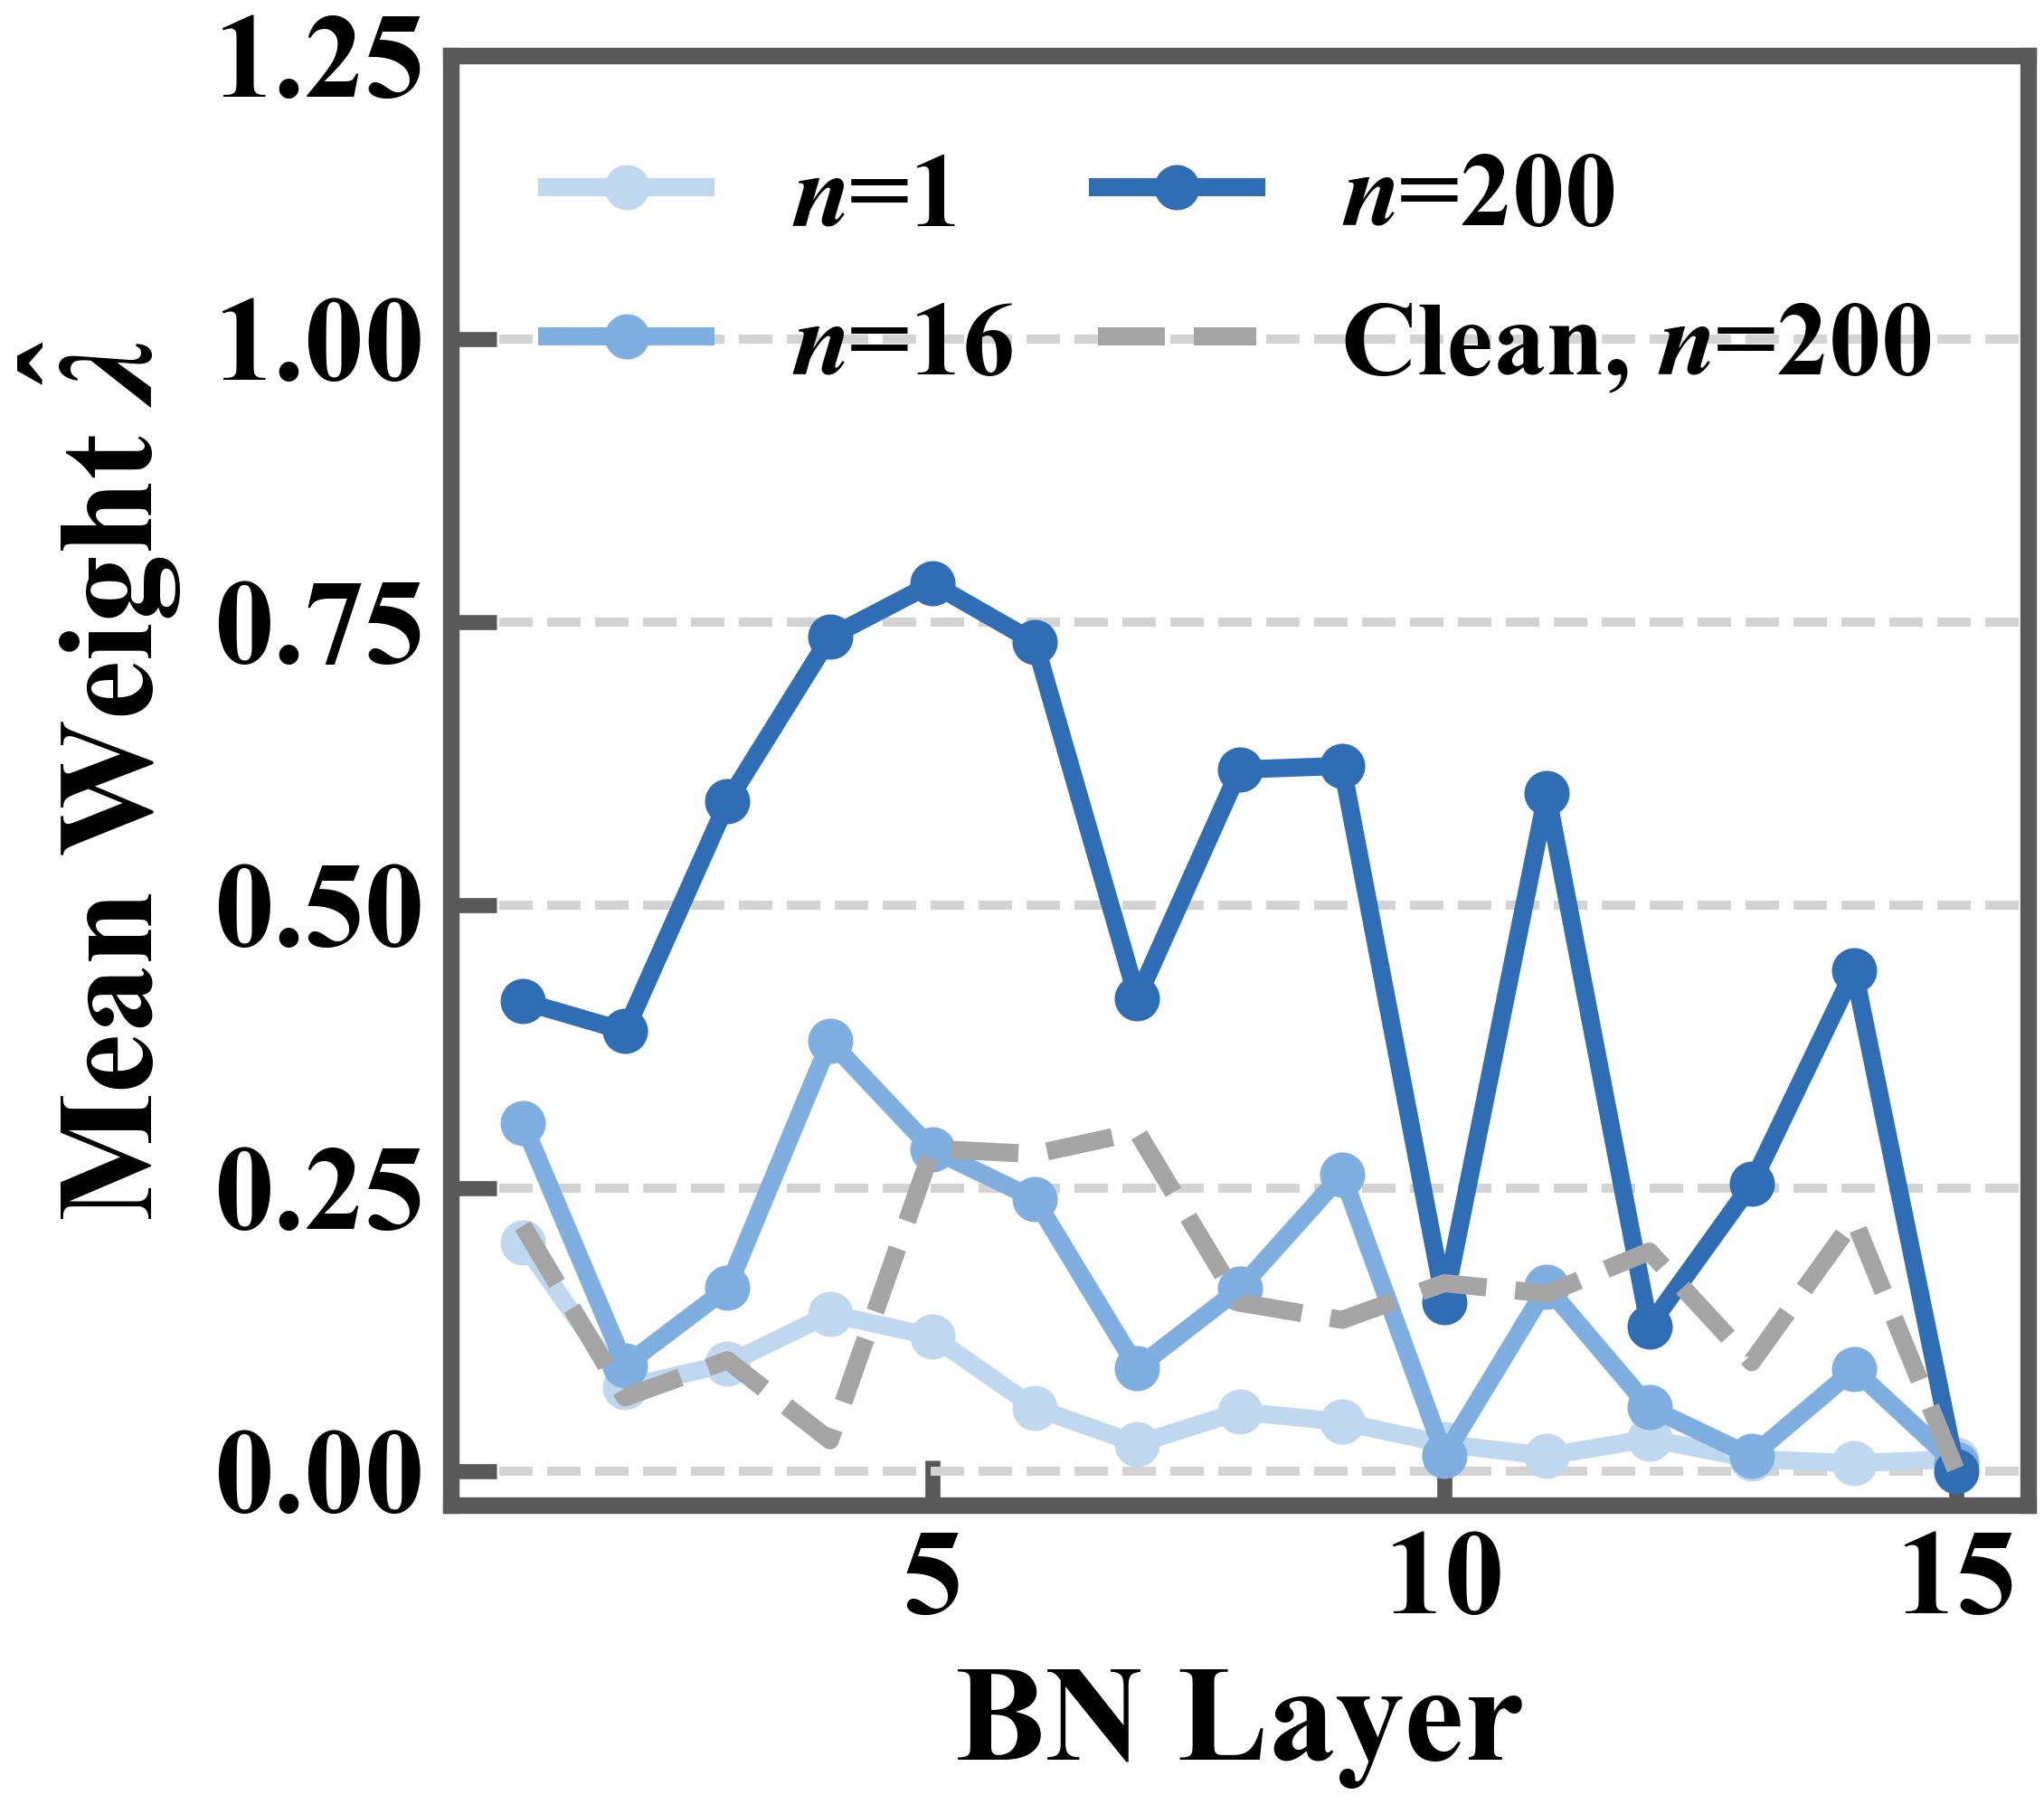
\includegraphics[width=\linewidth]{figures/exp/mechanism/lambda_by_layer_resnet14.png}
        \caption{ResNet-14.}
        \label{fig:lambda-a}
    \end{subfigure}\hfill
    \begin{subfigure}[t]{0.49\columnwidth}
        \centering
        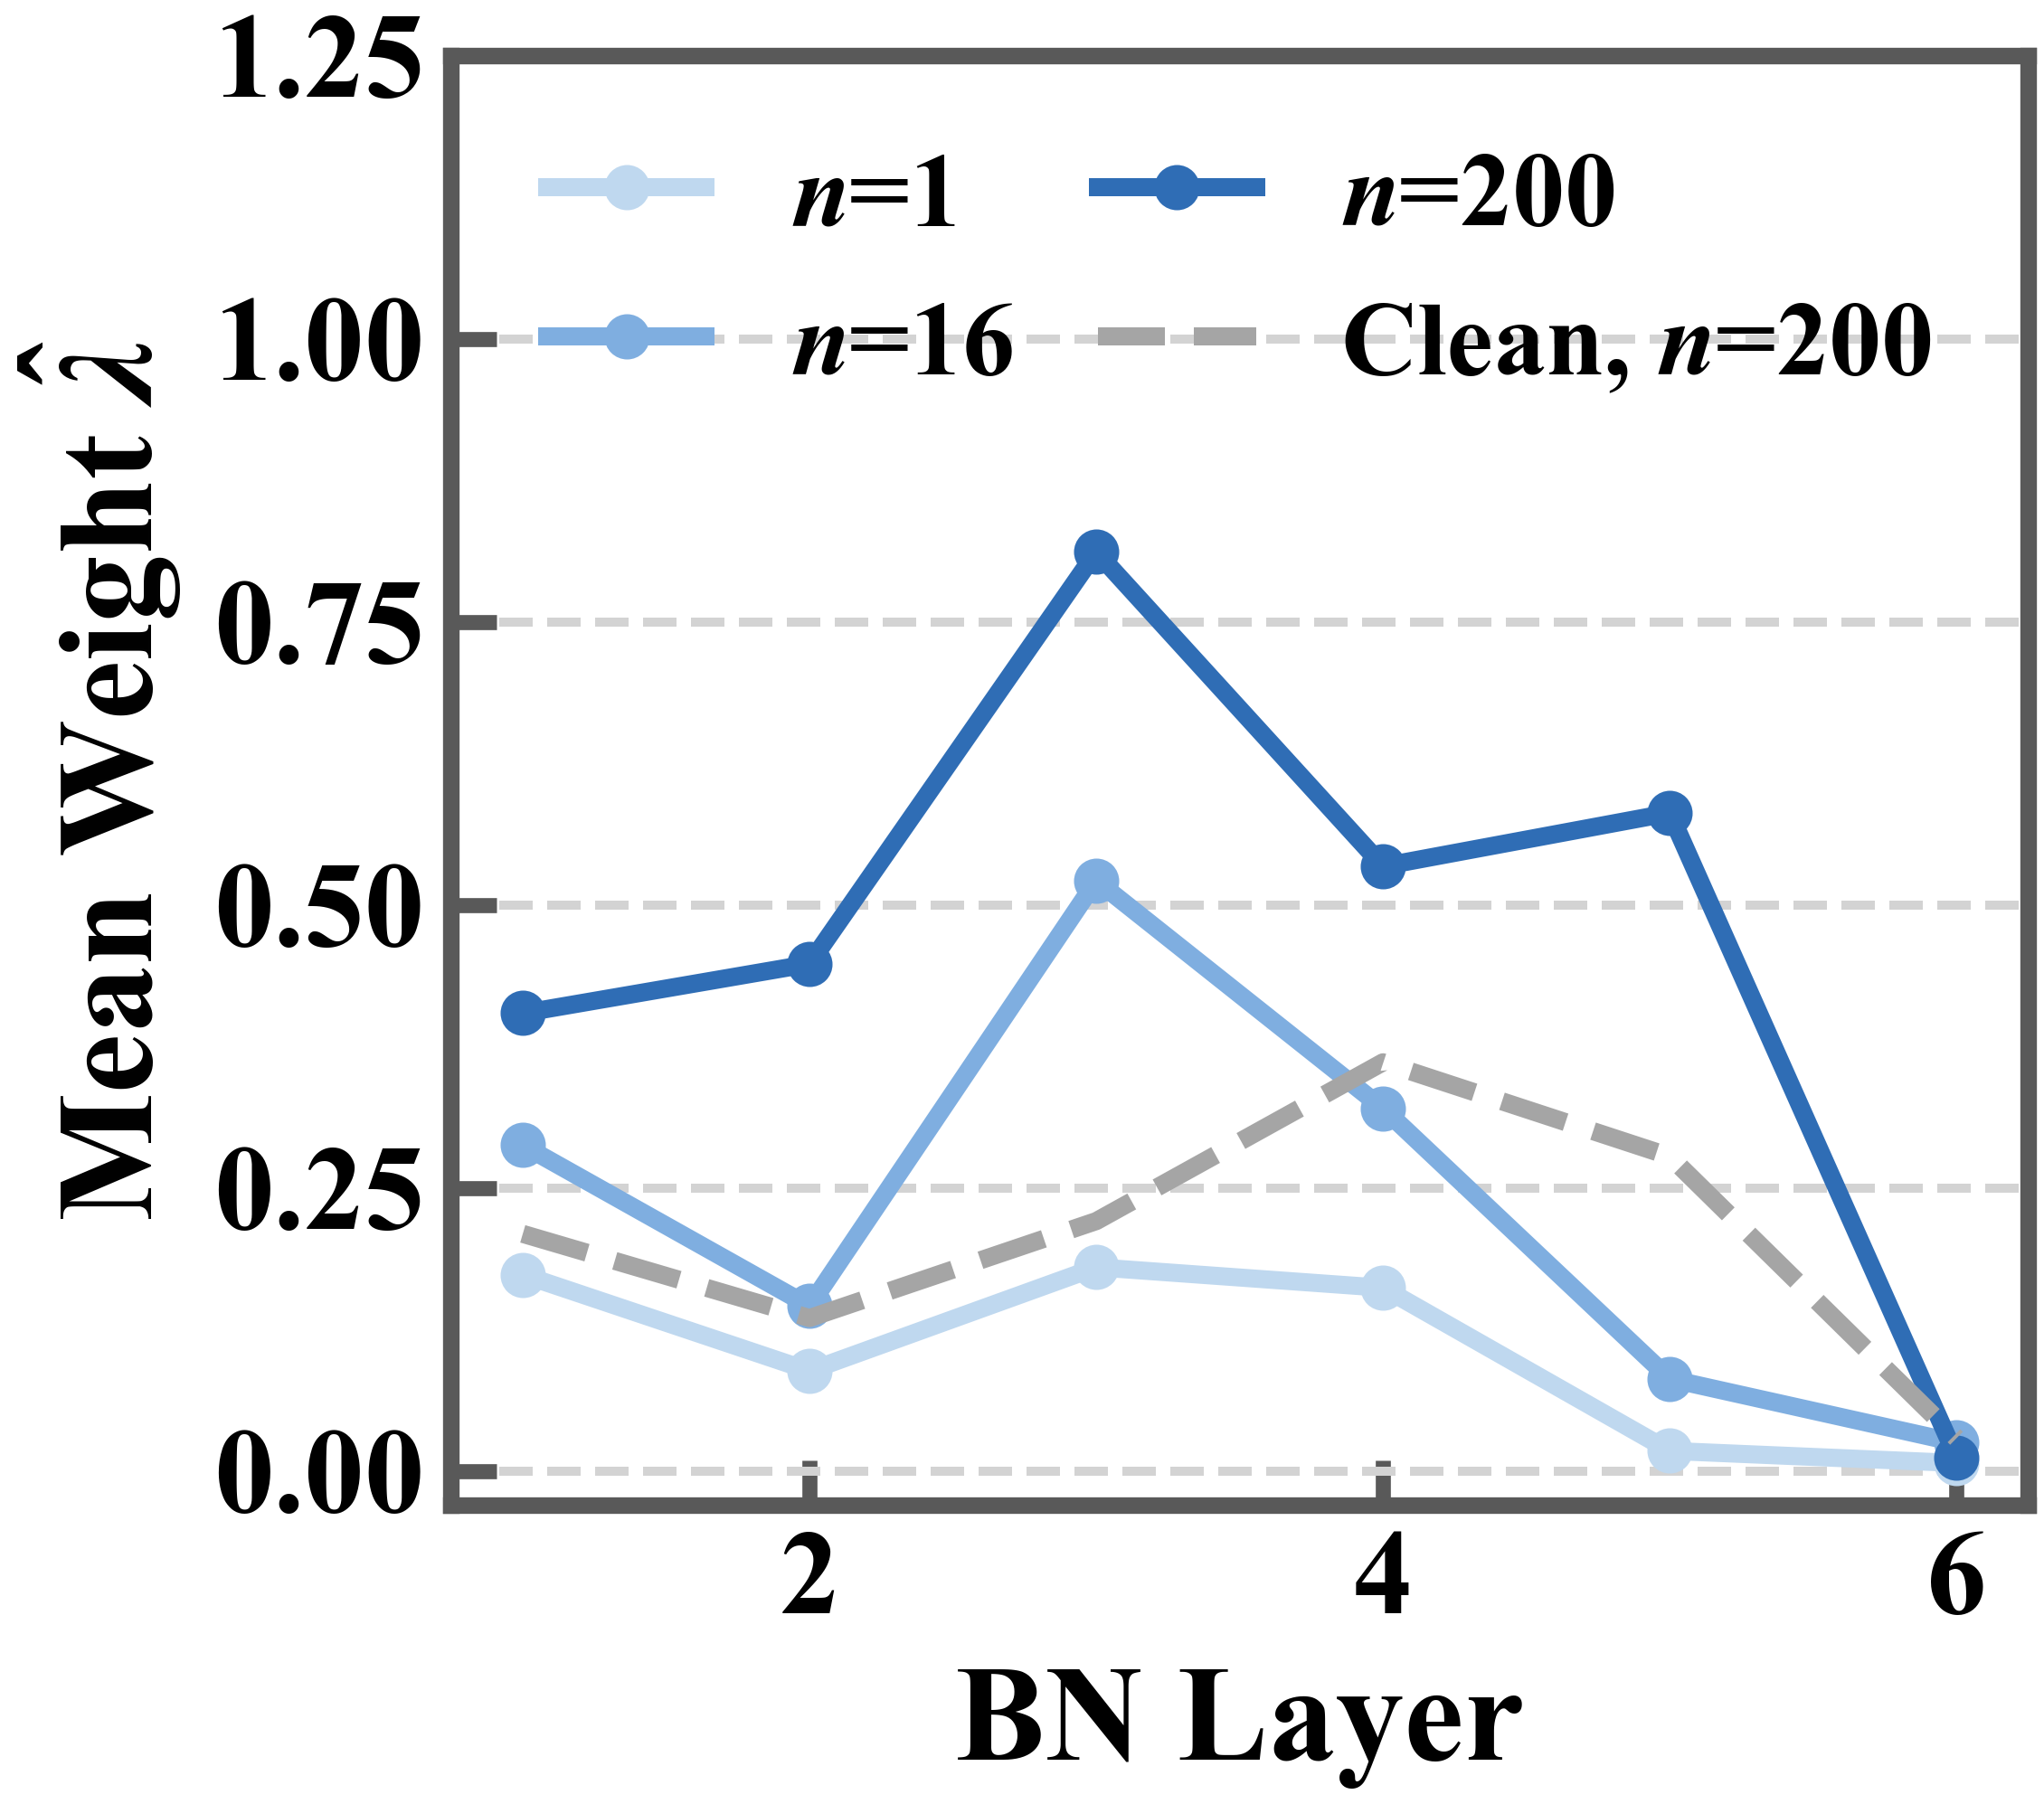
\includegraphics[width=\linewidth]{figures/exp/mechanism/lambda_by_layer_cnn8.png}
        \caption{CNN-8.}
        \label{fig:lambda-b}
    \end{subfigure}
    \caption{Stein weight $\hat{\lambda}_{\mu}$ per BN layer, averaged over test batches and the 15 corruptions at severity 5, for three batch sizes; the dashed line is clean data at $n{=}200$.}
    \label{fig:lambda}
    \vspace{-12pt}
\end{figure}

\textbf{Estimation variance.} To isolate the estimator from the network, we simulate per-sample means with $C{=}64$ channels and a known noise level, as in Figure~\ref{fig:teaser-figure}.
For batch sizes from 1 to 64, the risk of SourceStein is at most 0.023 per channel above that of the oracle weight and never above that of TBN, consistent with Proposition~\ref{prop:risk}.
Figure~\ref{fig:robust} breaks the two assumptions of the proposition.
With heavy-tailed noise (\ref{fig:robust-a}), SourceStein remains below TBN at each shift and at most 0.114 per channel above the oracle.
When the true noise is smaller than the stored level (\ref{fig:robust-b}), the score understates the evidence for a shift, and SourceStein exceeds TBN at 6 of 14 shift sizes; Appendix~\ref{apdx:synthetic} adds further settings.
\begin{figure}[t]
    \centering
    \begin{subfigure}[t]{0.49\columnwidth}
        \centering
        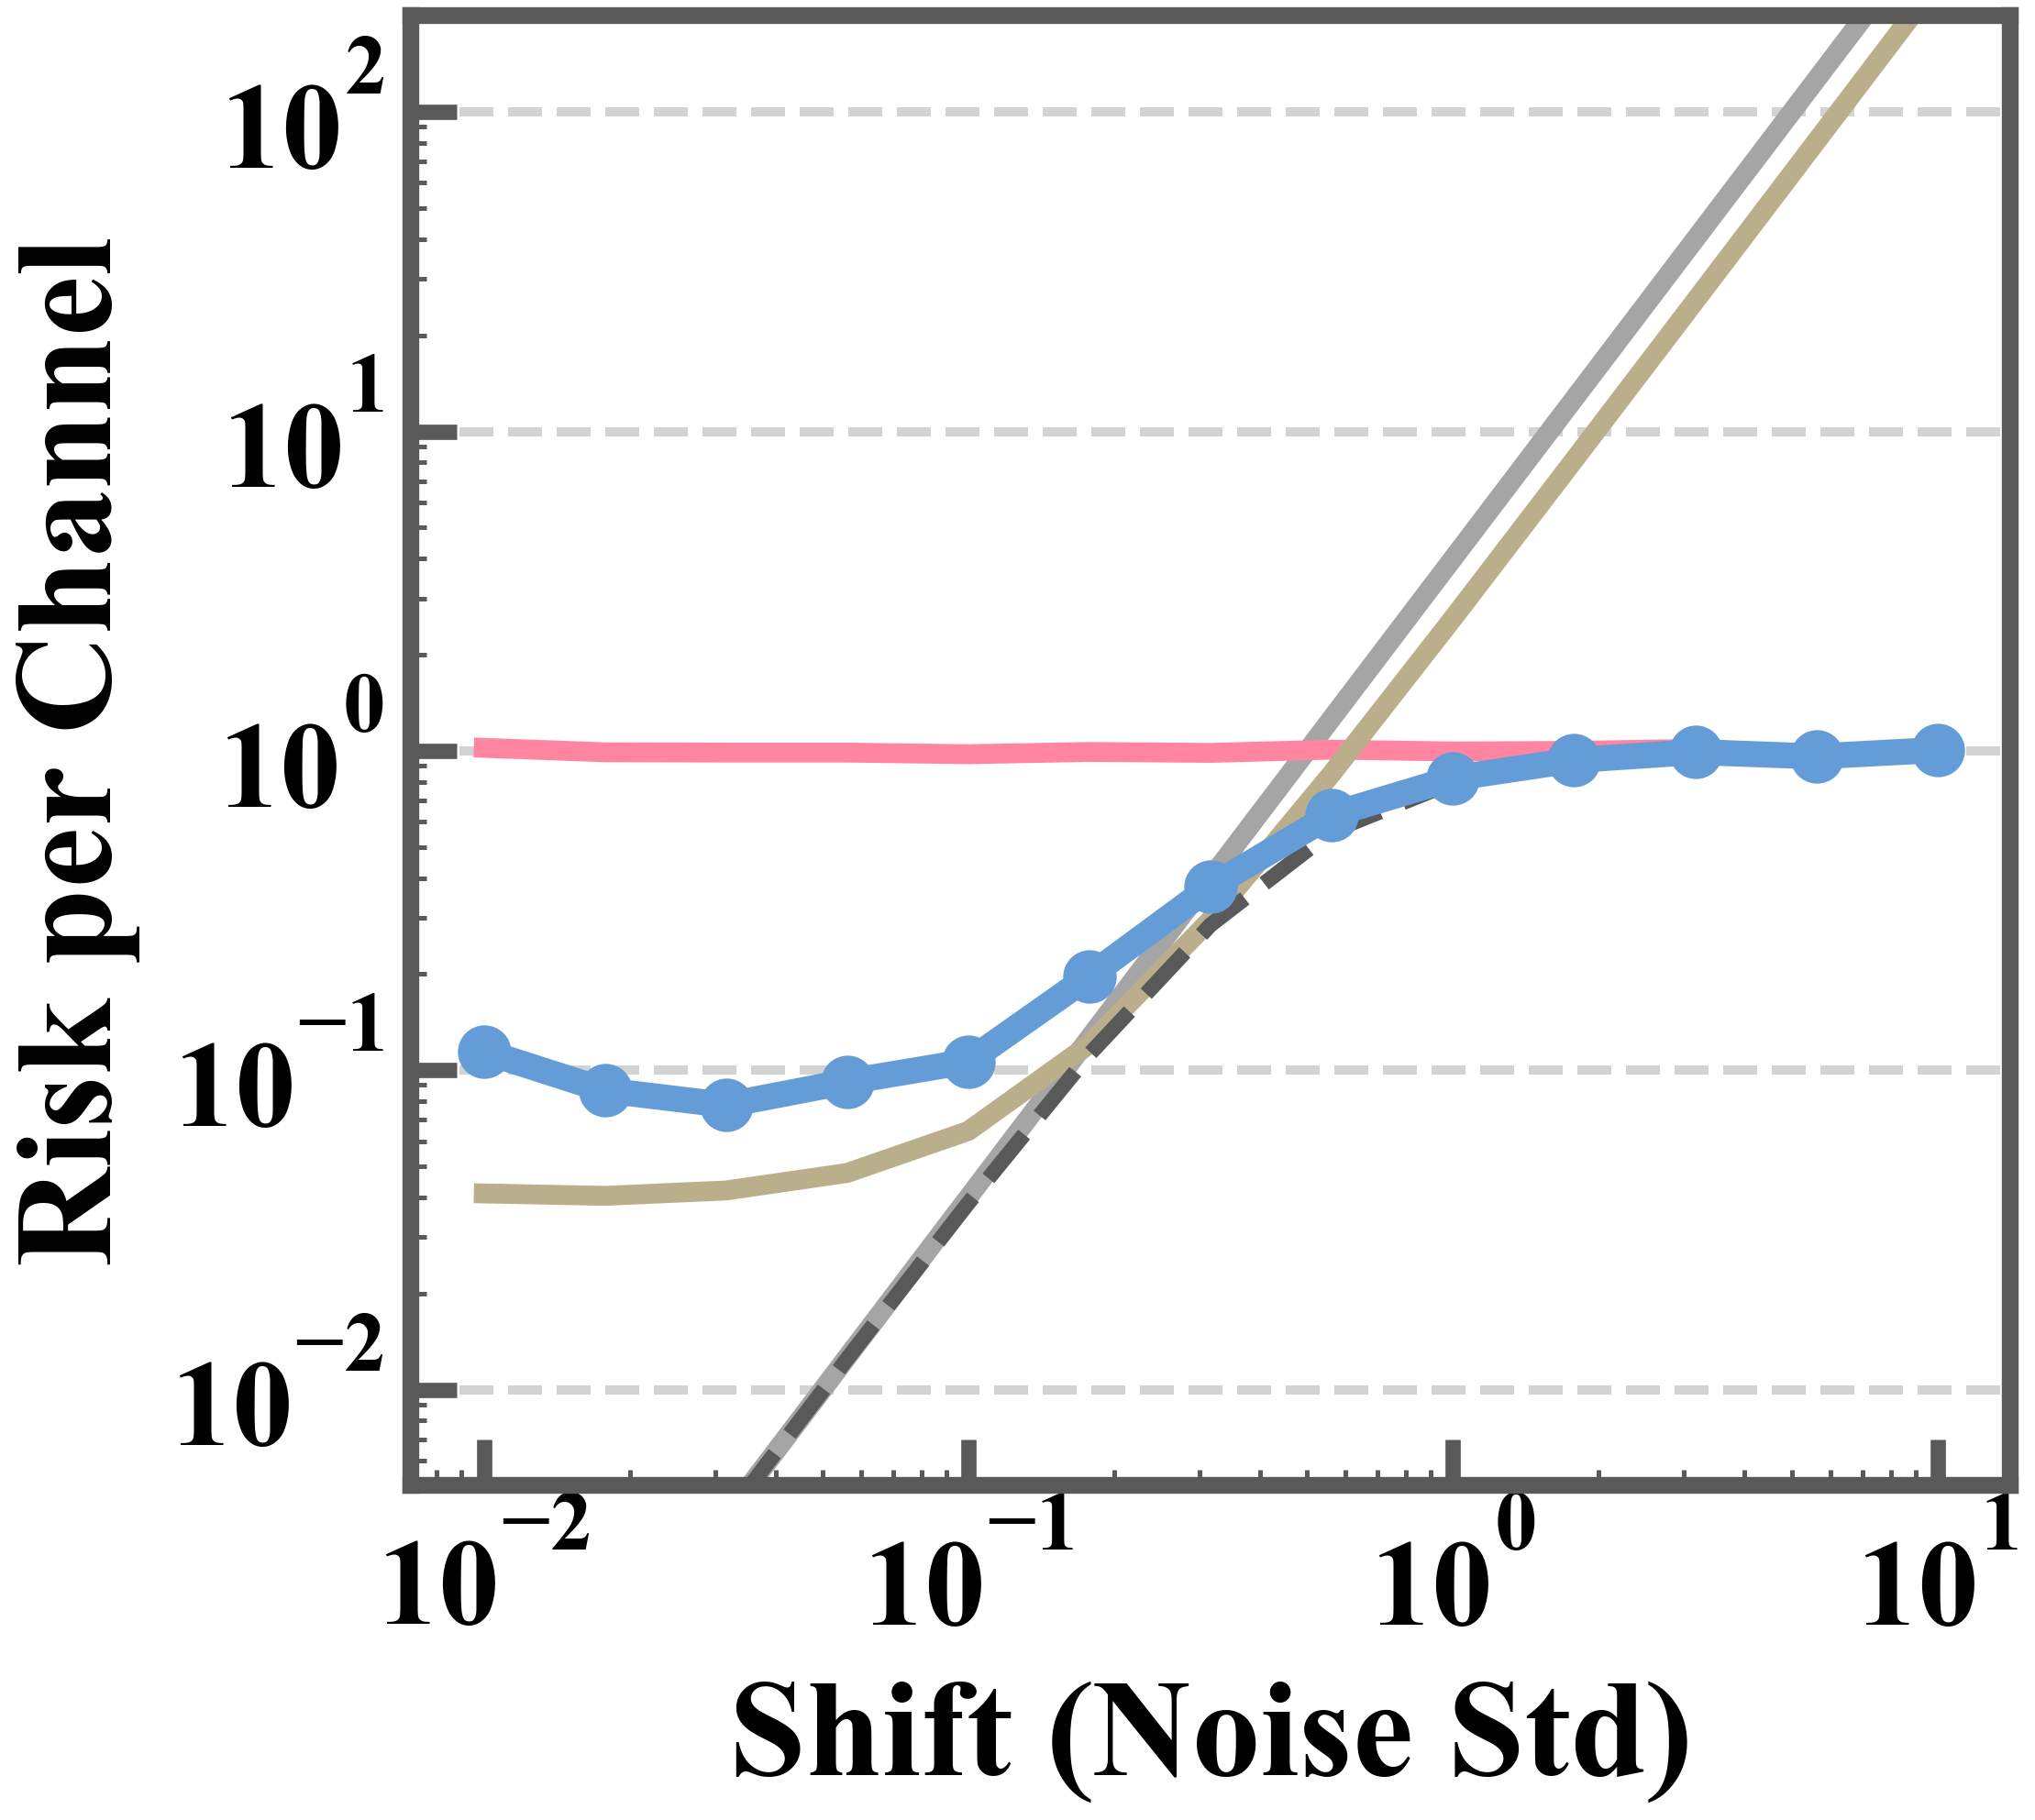
\includegraphics[width=\linewidth]{figures/exp/synthetic/risk_n4_student_t3_s1p0.png}
        \caption{Student-$t_3$ noise.}
        \label{fig:robust-a}
    \end{subfigure}\hfill
    \begin{subfigure}[t]{0.49\columnwidth}
        \centering
        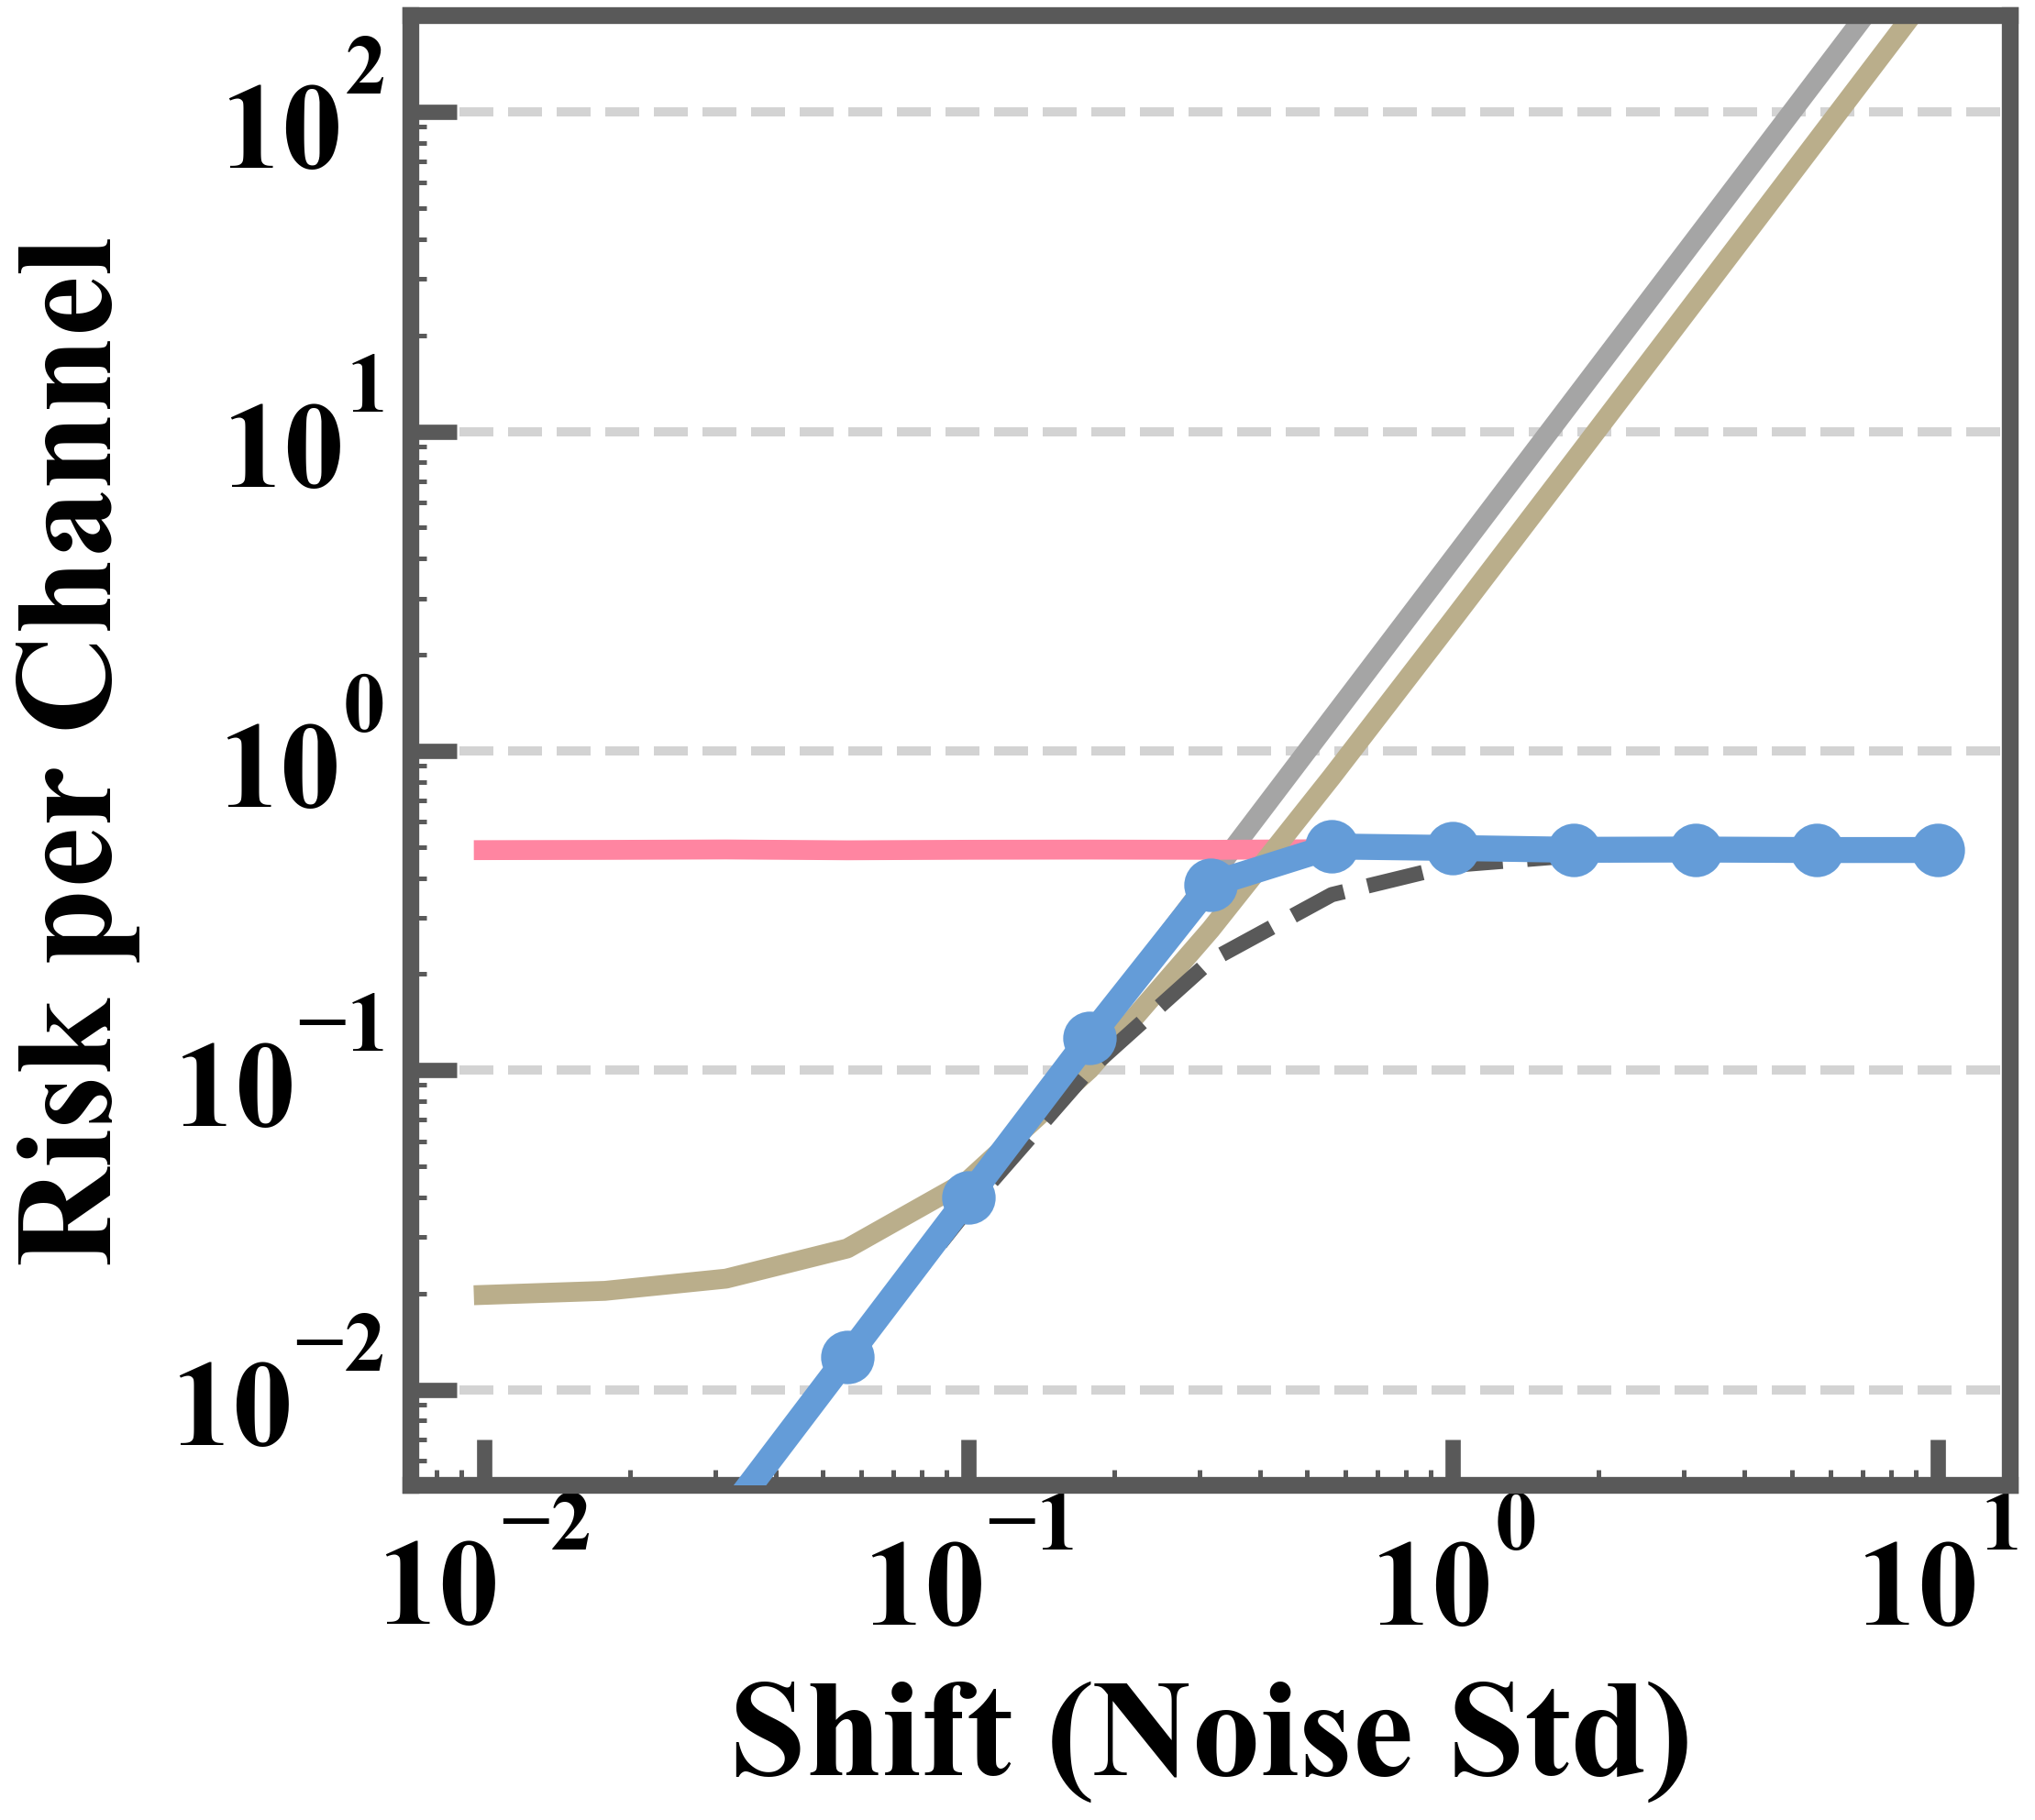
\includegraphics[width=\linewidth]{figures/exp/synthetic/risk_n4_gauss_s0p7.png}
        \caption{Noise $0.7\times$ the stored level.}
        \label{fig:robust-b}
    \end{subfigure}
    \caption{Simulated risk per channel at $n{=}4$ when the assumptions of Proposition~\ref{prop:risk} fail, with the legend of Figure~\ref{fig:teaser-figure}.}
    \label{fig:robust}
    \vspace{-12pt}
\end{figure}

These results indicate that the gains of Table~\ref{tab:main-table} come from a weight that follows the shift while remaining near zero when the batch contains little evidence.

\subsection{(RQ3) Ablation Study} \label{sec:ablation-study}
To examine which parts of SourceStein matter, we remove one design choice at a time and report the results in Table~\ref{tab:ablation}.

\begin{table}[t]
\centering
\renewcommand{\arraystretch}{0.9}
\caption{Ablation of SourceStein: error (\%) on CIFAR-10-C at severity 5. The best result in each column of a block is \textbf{bold}.}
\label{tab:ablation}
\shrinktofit{\columnwidth}{%
\begin{tabular}{cl|cccc}
\toprule
 & & \multicolumn{4}{c}{\textbf{Test Batch Size $n$}} \\
 & \textbf{Variant} & \textbf{1} & \textbf{4} & \textbf{16} & \textbf{64} \\
\midrule
\multirow{5}{*}{\rotatebox{90}{ResNet-14}}
 & \cellcolor{oursrowblue}SourceStein & \cellcolor{oursrowblue}\textbf{45.34} & \cellcolor{oursrowblue}\textbf{36.23} & \cellcolor{oursrowblue}\textbf{32.50} & \cellcolor{oursrowblue}31.00 \\
 & w/o pooling & 46.16 & 36.51 & 32.69 & 31.01 \\
 & w/o variance weight & 46.41 & 37.28 & 32.76 & 31.21 \\
 & w/o variance adaptation & 49.69 & 44.78 & 40.76 & 37.85 \\
 & w/ batch noise level & \textbf{45.34} & 38.97 & 32.77 & \textbf{30.95} \\
\midrule\midrule
\multirow{5}{*}{\rotatebox{90}{CNN-8}}
 & \cellcolor{oursrowblue}SourceStein & \cellcolor{oursrowblue}43.93 & \cellcolor{oursrowblue}\textbf{34.65} & \cellcolor{oursrowblue}30.43 & \cellcolor{oursrowblue}28.32 \\
 & w/o pooling & 46.05 & 35.02 & \textbf{30.16} & 28.11 \\
 & w/o variance weight & \textbf{43.50} & 36.13 & 31.68 & 29.49 \\
 & w/o variance adaptation & 51.39 & 47.51 & 46.25 & 46.33 \\
 & w/ batch noise level & 43.93 & 37.99 & 30.26 & \textbf{28.09} \\
\bottomrule
\end{tabular}}
\vspace{-10pt}
\end{table}

\textbf{Impact of each component.} The first variant replaces the pooled Stein weight by a separate weight per channel (w/o pooling).
The next two reuse the mean weight for the variance (w/o variance weight) or keep the source variance (w/o variance adaptation).
The last estimates $\boldsymbol{\tau}^2$ and $\boldsymbol{\rho}^2$ from the test batch (w/ batch noise level), with the source values at $n{=}1$.
We have the following observations: \textbf{adapting the variance matters most, and pooling helps mainly for small batches.}
Keeping the source variance increases the error by 4 to 18 points at each batch size.
This suggests that much of the corruption shift lies in the feature scale.
Moreover, per-channel weights are worse at $n \le 4$ on both networks but slightly better at $n \ge 16$ on CNN-8, consistent with pooling being most useful when each channel contains little evidence.
Additionally, estimating the noise level from the test batch statistics hurts at $n{=}4$ by 2.7 to 3.3 points, since a variance from four samples is itself noisy.

\begin{figure}[t]
    \centering
    \begin{subfigure}[t]{0.49\columnwidth}
        \centering
        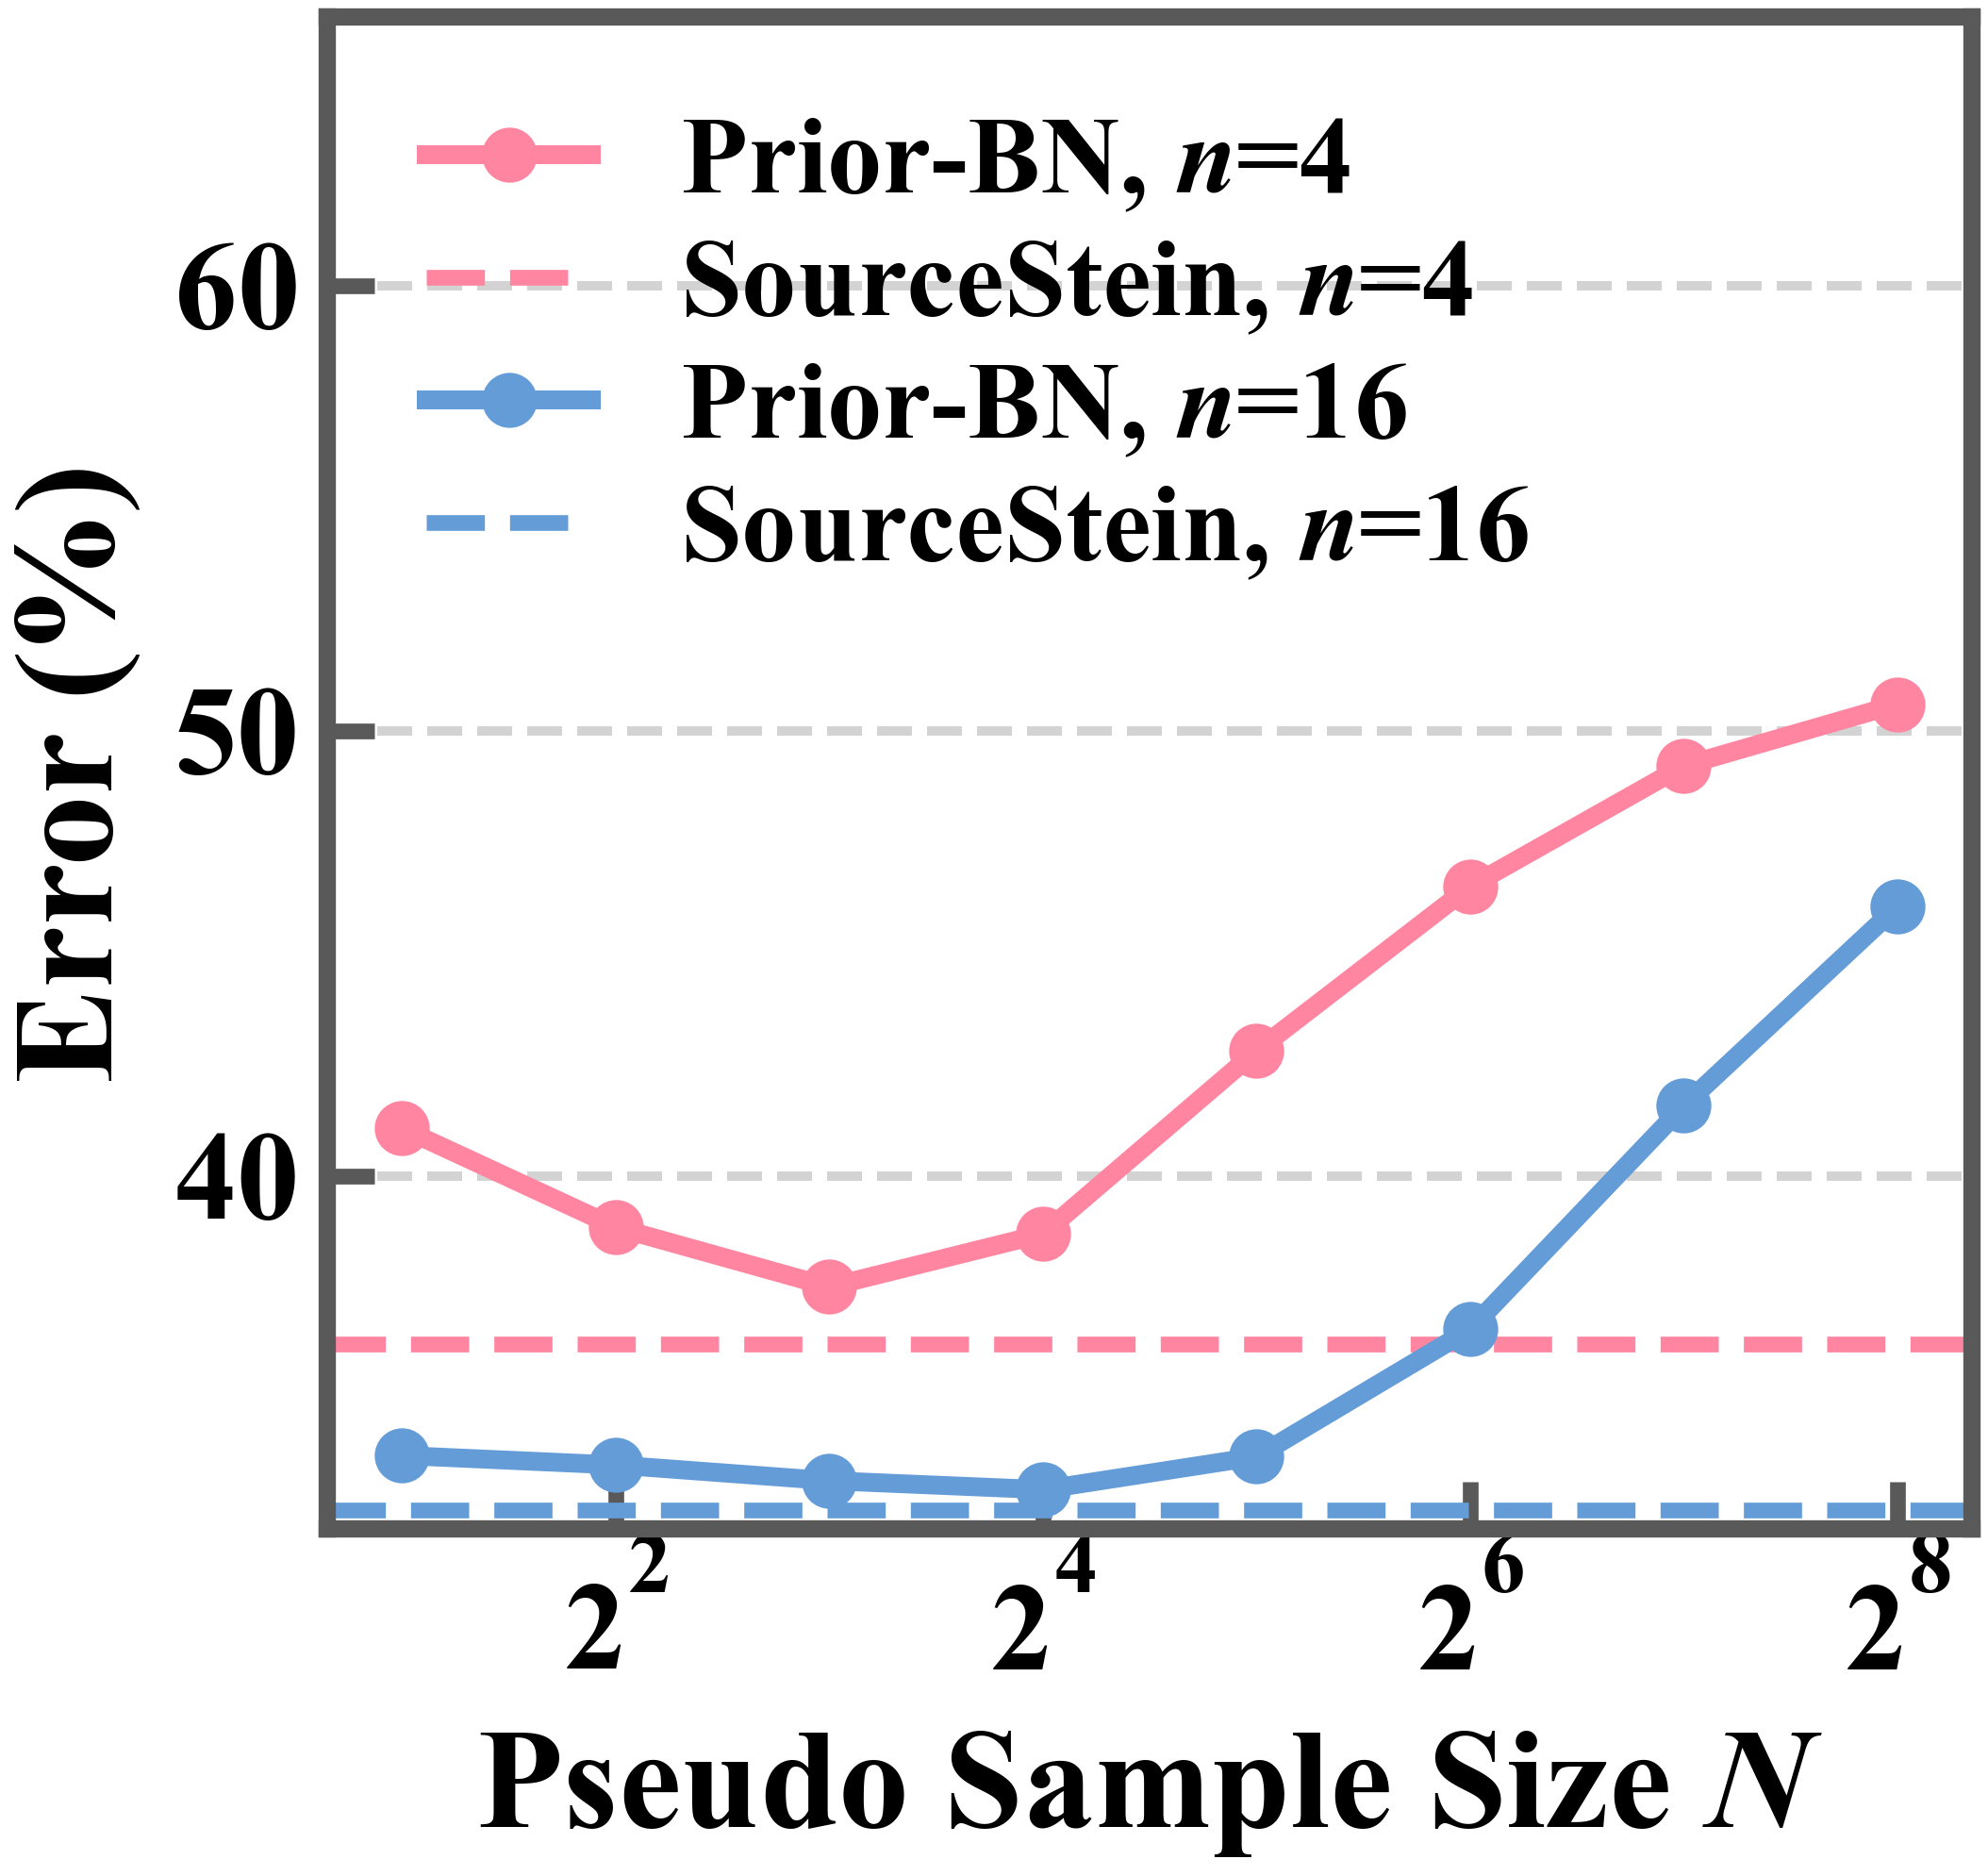
\includegraphics[width=\linewidth]{figures/exp/ablation/prior_sweep_resnet14.png}
        \caption{ResNet-14.}
        \label{fig:prior-n-a}
    \end{subfigure}\hfill
    \begin{subfigure}[t]{0.49\columnwidth}
        \centering
        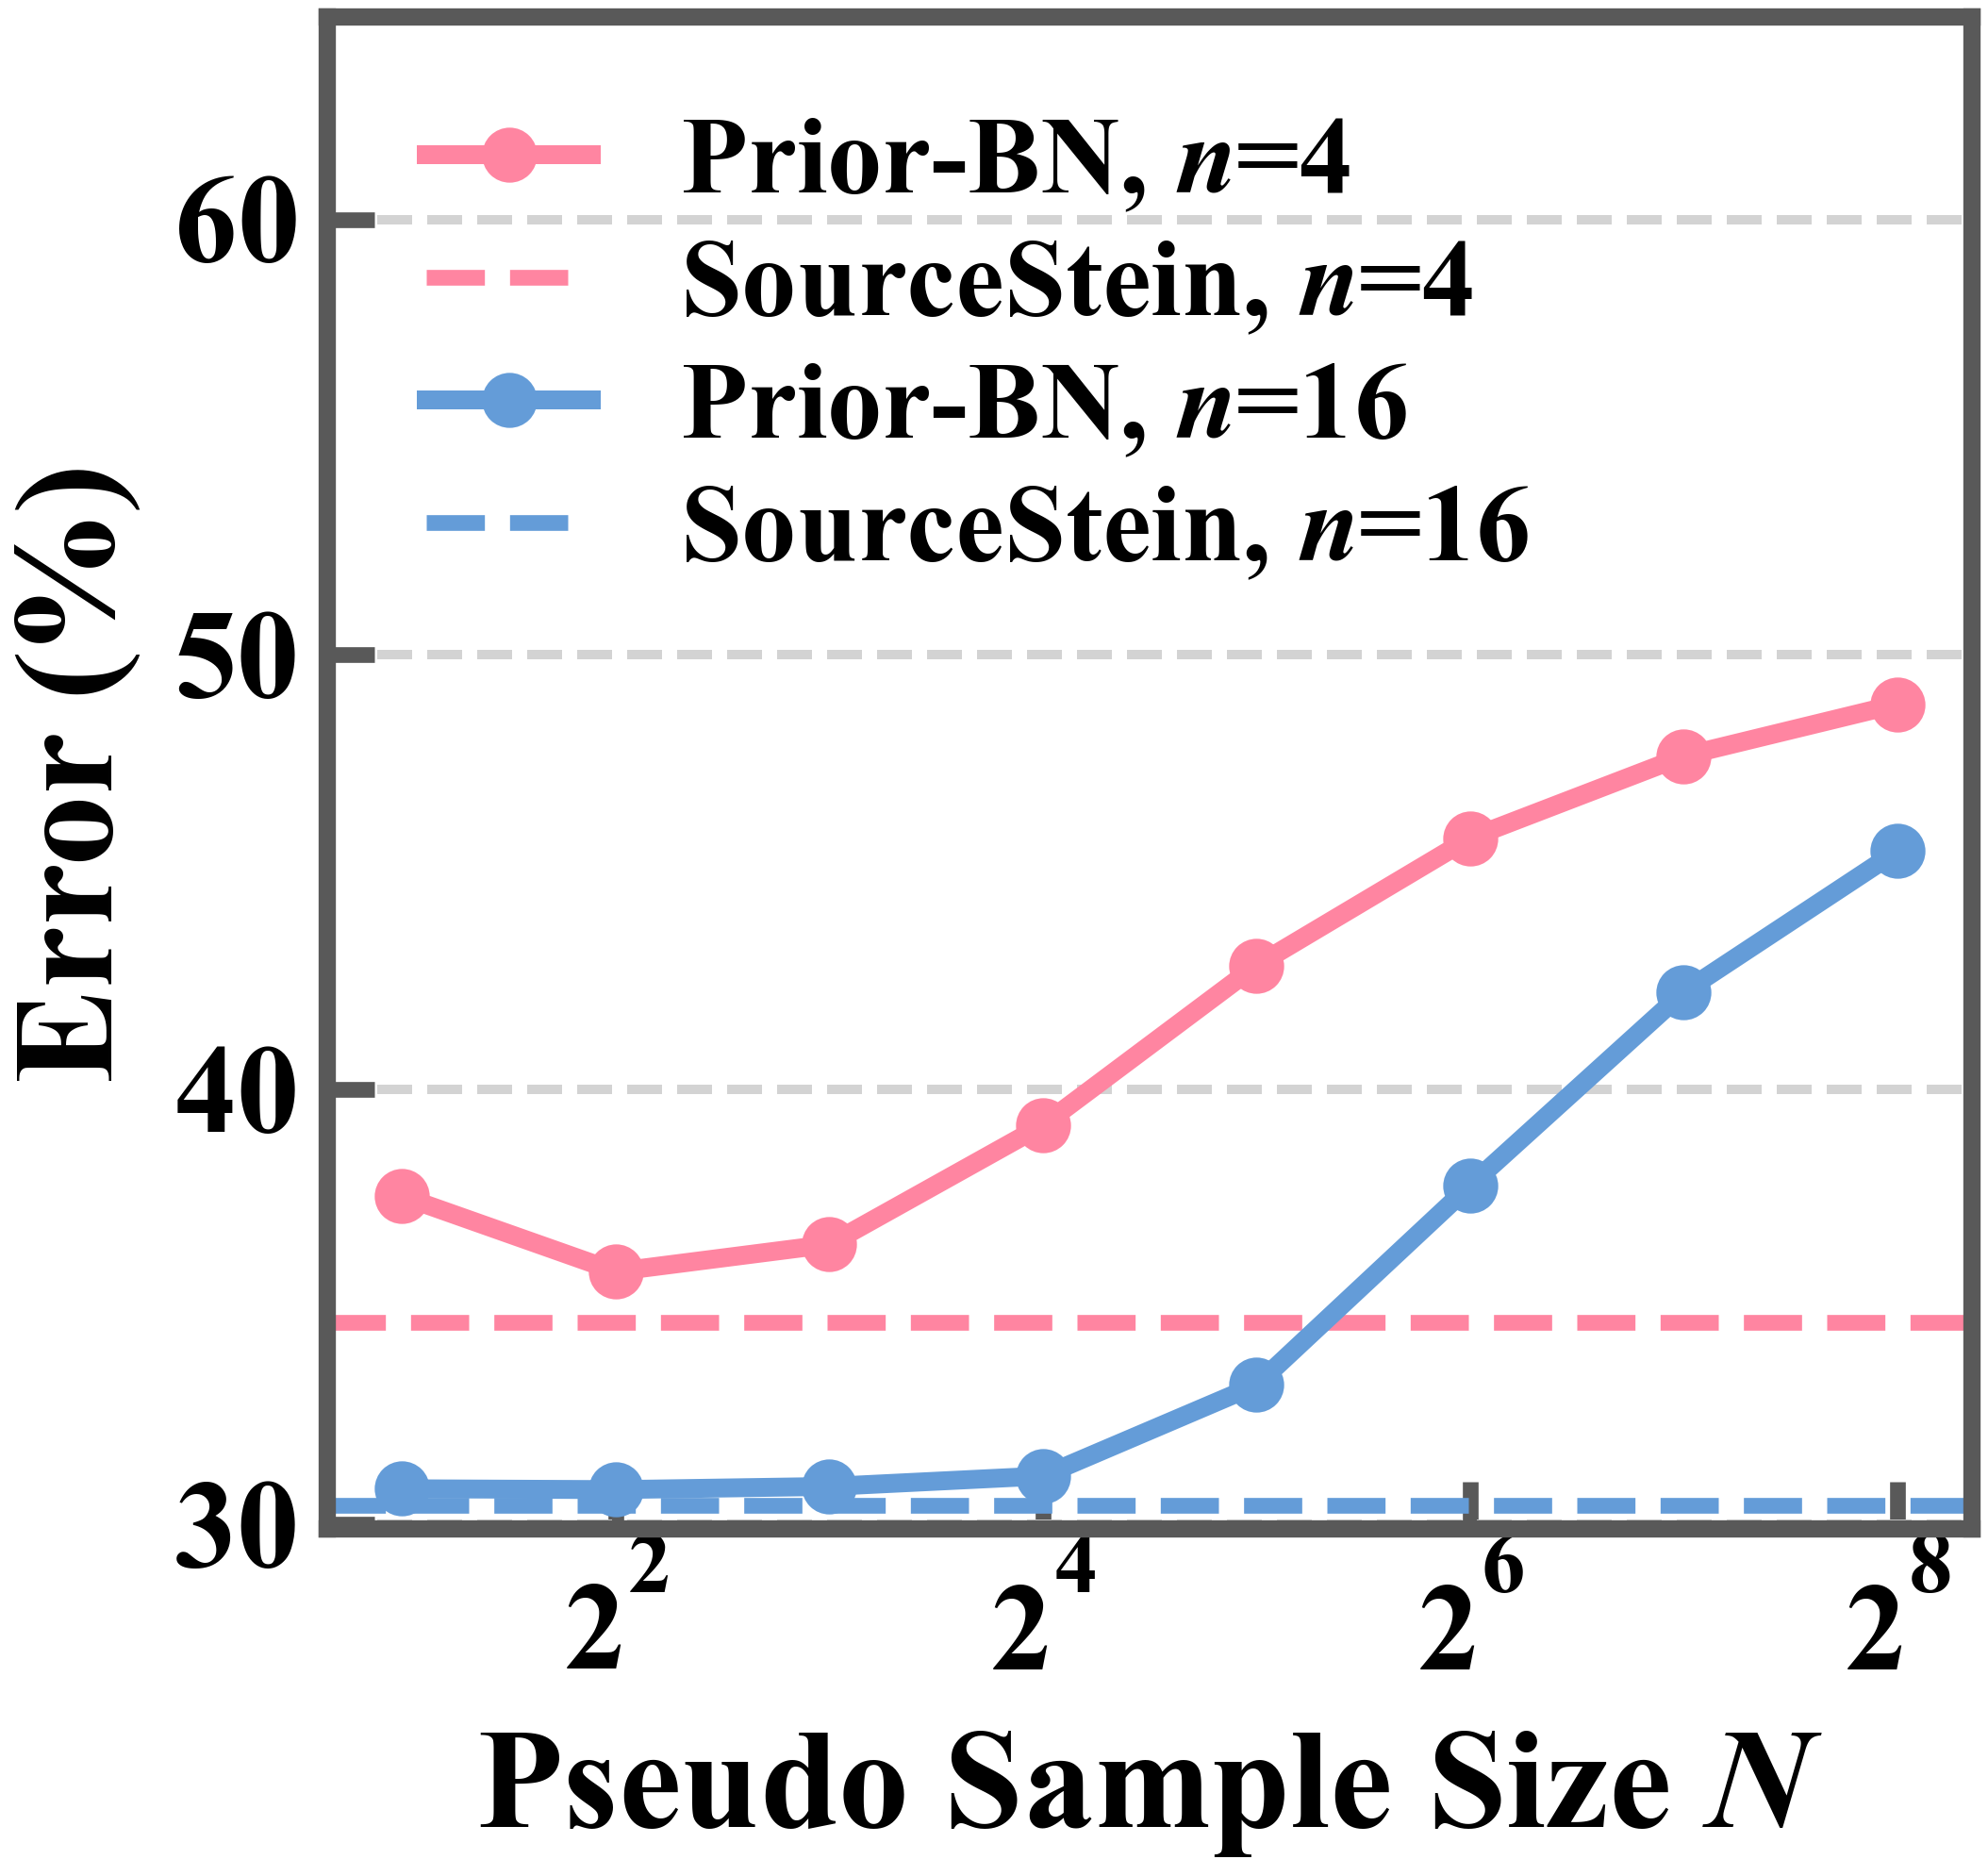
\includegraphics[width=\linewidth]{figures/exp/ablation/prior_sweep_cnn8.png}
        \caption{CNN-8.}
        \label{fig:prior-n-b}
    \end{subfigure}
    \caption{Error of Prior-BN over its pseudo sample size $N$ for $n{=}4$ and $n{=}16$; dashed lines mark SourceStein at the same batch size.}
    \label{fig:prior-n}
    \vspace{-12pt}
\end{figure}

\textbf{Comparison with each pseudo sample size.} Figure~\ref{fig:prior-n} varies $N$ of Prior-BN from 2 to 256.
At $n{=}4$ and $n{=}16$, no value of $N$ reaches the error of SourceStein on either network, and the best $N$ itself moves with the batch size and the network (from 2 to 64; Appendix~\ref{apdx:impl-details}).
Such results show that the per-batch weight of SourceStein replaces a hyperparameter that would otherwise require labelled shifted data.

\subsection{(RQ4) Combination with Entropy Minimization} \label{sec:extension}
Finally, we test whether SourceStein can serve as the normalization inside TENT \cite{TENT}, which updates the BN affine parameters online by entropy minimization.
We take one Adam step per batch with learning rate $10^{-3}$ and reset the model for each corruption.

\begin{table}[t]
\centering
\renewcommand{\arraystretch}{0.9}
\caption{Error (\%) of TENT with three normalization rules on CIFAR-10-C at severity 5. The best result in each column is \textbf{bold}.}
\label{tab:tent}
\shrinktofit{\columnwidth}{%
\begin{tabular}{l|ccc|ccc}
\toprule
 & \multicolumn{3}{c|}{\textbf{ResNet-14}} & \multicolumn{3}{c}{\textbf{CNN-8}} \\
\textbf{Normalization} & $n{=}4$ & $n{=}16$ & $n{=}64$ & $n{=}4$ & $n{=}16$ & $n{=}64$ \\
\midrule
TBN & 45.15 & 33.72 & 31.07 & \textbf{42.85} & \textbf{30.99} & \textbf{27.93} \\
Prior-BN & 64.17 & 33.12 & \textbf{30.86} & 66.31 & 31.85 & 28.42 \\
\rowcolor{oursrowblue} SourceStein & \textbf{43.82} & \textbf{33.09} & 31.10 & 44.98 & 31.31 & 28.49 \\
\bottomrule
\end{tabular}}
\vspace{-10pt}
\end{table}

As shown in Table~\ref{tab:tent}, we have the following observation: \textbf{the gain of SourceStein extends to entropy minimization on ResNet-14 but not on CNN-8.}
TENT with SourceStein is the best of the three rules on ResNet-14 for $n \le 16$, while TENT with TBN is lower on CNN-8 at each batch size.
A likely reason is that TENT already adapts the affine parameters to the test data.
The gradient steps may then not correct the part of the shift bias that SourceStein leaves in the statistics, while TBN removes the full shift before them.
Prior-BN with $N{=}16$ collapses at $n{=}4$ on both networks, which indicates that a fixed weight can interact badly with online updates.
Moreover, all three rules use the learning rate of \citet{TENT}, and a learning rate tuned for each rule may change this ranking.
Overall, SourceStein is most useful as a training-free rule, and its combination with gradient-based adaptation remains network-dependent.

\section{Limitations} \label{sec:limitations}
This work still has a few limitations.
On the one hand, the guarantee of Proposition~\ref{prop:risk} assumes Gaussian batch means with a noise level measured on source data, and Oracle-$N$ remains lower at batch size one.
On the other hand, we evaluate two small networks on synthetic corruptions, and whether the rule helps on larger models, natural shifts or non-i.i.d.\ streams is still unknown.

\section{Conclusion} \label{sec:conclusion}
Test-time normalization methods mix source statistics and test batch statistics with a mixing weight fixed in advance, which leaves stale source statistics under large shifts and noisy batch statistics under small batches.
To address both, this work presented SourceStein, an adaptive and stable rule that sets the weight of each layer from the batch by James--Stein shrinkage toward the source statistics.
We showed that, under a Gaussian model, its risk never exceeded that of the batch statistics and remained close to the best fixed weight, balancing the shift bias and the estimation variance.
Experiments on common corruptions showed that SourceStein generally reduced the error of prior mixing rules for small batches while matching them for large ones.
We will further explore shrinkage targets that combine the source statistics with earlier test batches.
\label{main-text-end}
         % Limitations + Conclusion; \label{main-text-end}

% --- Not counted toward the page limit (ICML 2026 CFP) ---------------------
\clearpage                            % statements start a fresh page, so the
                                      % main body visibly ends on p8 (p9 CR)
\section*{AI Disclosure Statement}
% Required by ICML 2027 (CFP "Use of Generative AI by Authors & Disclosure Policy"); kit heading: AI Use Statement.
This submission was produced with substantive use of a generative AI agent (a large language model with code-execution tools).
The agent proposed the research idea, wrote the experimental code, ran all experiments, analysed the results, drew the figures and tables, searched and checked the literature, and drafted the manuscript.
Each number in the paper is read from the raw output files of the released code, and each reference was compared with its arXiv or publisher record.
The authors are responsible for reviewing all AI-generated content, including code, results, mathematical claims and citations, and take full responsibility for the paper.

\section*{Impact Statement}
% Mandatory for the main track (ICML 2027 CFP "Impact Statements"); house three-sentence pattern.
This work aims to make test-time normalization of deployed image classifiers more adaptive and stable when only a few test inputs arrive at a time, which can help applications such as on-device perception under changing sensors or weather.
We expect its main societal effect to be positive, since a model that degrades less under distribution shift makes fewer silent errors.
One risk is that a lower error under synthetic corruptions may be read as robustness to all real-world shifts, which our experiments do not establish.

% Camera-ready only (never at submission: CFP / Author Instructions forbid
% acknowledgements and grant numbers in the blind version):
% \section*{Acknowledgements}
% This research is supported by <grant> (<number>).

\bibliography{example_paper}
\bibliographystyle{icml2027}

% The appendix switch only. \onecolumn is the template's default and the house
% layout keeps it [venue: ICML]; in the one-column appendix
% \columnwidth = \textwidth = 6.75 in, so 0.49\columnwidth panels are 3.3 in.
\newpage
\appendix
\onecolumn
           % \newpage \appendix \onecolumn
% Appendix: A Related Works, B Proof, C Implementation Details, D Additional Experiments, E Simulation Study.
\section{Related Works} \label{apdx:related-works}

\subsection{Test-Time Normalization}
Re-estimating BN statistics on target data is a simple and widely adopted response to covariate shift.
AdaBN \cite{AdaBN} replaces the source statistics by target-domain statistics for domain adaptation, and prediction-time BN \cite{PredictionBN} and the covariate shift adaptation of \citet{BN-Adapt} recompute them on each test batch, \citet{BN-Adapt} with a pseudo sample size $N$ that mixes in the source statistics.
$\alpha$-BN \cite{AlphaBN} mixes the two with a constant weight, DUA \cite{DUA} updates them with a decaying momentum over the stream, TTN \cite{TTN} learns a per-layer interpolation in a post-training phase on source data, and UnMix-TNS \cite{UnMix-TNS} and NOTE \cite{NOTE} handle test streams whose labels are correlated in time.
While effective, such rules fix how much they trust a test batch in advance (by a hyperparameter, a schedule or weights learned on source data), and they remain exposed to stale source statistics under large shifts and to noisy batch statistics under small batches.

\subsection{Test-Time Adaptation with Gradient Updates}
A second line updates model parameters on the test data.
TENT \cite{TENT} minimizes the prediction entropy with respect to the BN affine parameters, SAR \cite{SAR} reports that BN makes such updates unstable for small batches and filters samples with large gradients, and DELTA \cite{DELTA} renormalizes test-time BN statistics and reweights classes to remove biased updates.
These methods all rely on some estimate of the normalization statistics, and Section~\ref{sec:extension} shows that the choice of this estimate changes their error.
However, how to set the statistics of each batch without any hyperparameter remains largely underexplored in this line.

\subsection{Shrinkage Estimation in Normalization Layers}
The James--Stein estimator \cite{James-Stein} improves the sample mean of three or more Gaussian means by shrinking it toward a fixed point, and the empirical Bayes view of \citet{Efron-Morris} explains the shrinkage factor as an estimate of the signal-to-noise ratio.
Recent work applies Stein shrinkage inside normalization layers during training: \citet{JS-Norm} shrink the batch means and variances of each layer toward their cross-channel average, and \citet{Stein-BN-Adv} prove that such shrinkage dominates the sample estimates under sub-Gaussian adversarial perturbations.
These methods shrink toward a centre computed from the same batch, during training, to reduce noise rather than to correct a shift.
To address these gaps, we propose SourceStein, which shrinks the test batch statistics toward the source statistics at test time, so that one closed-form weight per layer is adaptive and stable: it follows the shift when the batch contains evidence for it and keeps the source statistics otherwise.

\clearpage
\section{Proof of Proposition~\ref{prop:risk}} \label{apdx:proof}
\textbf{Setup.} Our goal is to bound the risk of Equation~\ref{eq:risk} at the Stein weight.
Let $\mathbf{z} = \sqrt{n}\,\boldsymbol{\Sigma}^{-1/2}\hat{\boldsymbol{\mu}}$, $\boldsymbol{\theta} = \sqrt{n}\,\boldsymbol{\Sigma}^{-1/2}\boldsymbol{\mu}^{\text{tgt}}$ and $\mathbf{a} = \sqrt{n}\,\boldsymbol{\Sigma}^{-1/2}\boldsymbol{\mu}^{\text{src}}$.
Under the assumption $\hat{\boldsymbol{\mu}} \sim \mathcal{N}(\boldsymbol{\mu}^{\text{tgt}}, \boldsymbol{\Sigma}/n)$, we have $\mathbf{z} \sim \mathcal{N}(\boldsymbol{\theta}, \mathbf{I}_C)$.
For any weight $\lambda$, possibly depending on $\mathbf{z}$, the whitening is linear, so:
\begin{equation*}
n\,\|\boldsymbol{\mu}(\lambda) - \boldsymbol{\mu}^{\text{tgt}}\|^2_{\boldsymbol{\Sigma}^{-1}} = \|\mathbf{a} + \lambda(\mathbf{z} - \mathbf{a}) - \boldsymbol{\theta}\|^2,
\end{equation*}
and the shift score of Equation~\ref{eq:shift-score} is $S = \|\mathbf{z} - \mathbf{a}\|^2$.

\textbf{Risk of the Stein weight.} With $\lambda = 1 - (C-2)/S$, the estimator $\mathbf{a} + \lambda(\mathbf{z} - \mathbf{a})$ is the James--Stein estimator with target $\mathbf{a}$, whose risk is $C - (C-2)^2\,\mathbb{E}[1/S]$ by Lemma~\ref{lemma:james-stein}; the positive part $\hat{\lambda}$ of Equation~\ref{eq:stein-weight} has no larger risk \cite{Efron-Morris}.
Since $S$ follows a noncentral $\chi^2$ distribution with $C$ degrees of freedom and noncentrality $\|\boldsymbol{\theta} - \mathbf{a}\|^2 = \Delta$, we have $\mathbb{E}[S] = C + \Delta$.
Since the function $x \mapsto 1/x$ is convex on $(0, \infty)$, Jensen's inequality yields $\mathbb{E}[1/S] \ge 1/(C + \Delta)$, which is finite for $C \ge 3$.
We conclude:
\begin{equation*}
R(\hat{\lambda}) \le C - \frac{(C-2)^2}{C + \Delta} < C = R(1),
\end{equation*}
where $R(1) = \mathbb{E}\|\mathbf{z} - \boldsymbol{\theta}\|^2 = C$ is the risk of TBN.

\textbf{Excess over the oracle weight.} Subtracting $R(\lambda^{\star}) = C\Delta/(C + \Delta)$ from Equation~\ref{eq:oracle}:
\begin{equation*}
R(\hat{\lambda}) - R(\lambda^{\star}) \le \frac{C(C + \Delta) - (C-2)^2 - C\Delta}{C + \Delta} = \frac{4(C-1)}{C + \Delta} \le \frac{4(C-1)}{C} < 4.
\end{equation*}
Therefore, the bound holds for each shift $\boldsymbol{\delta}$ and batch size $n$, and the excess is largest without any shift ($\Delta = 0$), where the oracle keeps the source mean exactly. \hfill$\square$

\clearpage
\section{Implementation Details} \label{apdx:impl-details}
All experiments run on one CPU machine (15 cores, no GPU) with PyTorch\footnote{\url{https://pytorch.org}} 2.8 and NumPy; the code that produced each number is part of the supplementary material.

\textbf{Source models.} CNN-8 stacks three stages of two $3{\times}3$ convolutions with 32, 64 and 128 channels, each followed by BN and ReLU, with max pooling between stages, global average pooling and a linear head. ResNet-14 is the CIFAR residual network of \citet{ResNet} with two basic blocks per stage (widths 16, 32, 64), 15 BN layers in total. Table~\ref{tab:hyper} reports the training recipe; training took 11.6 min (CNN-8) and 11.9 min (ResNet-14) of wall-clock time on 7 threads each.

\begin{table}[ht]
\centering
\caption{Training and evaluation settings.}
\label{tab:hyper}
\begin{tabular}{l|c}
\toprule
\textbf{Setting} & \textbf{Value} \\
\midrule
Optimizer & SGD, Nesterov momentum 0.9, weight decay $5 \times 10^{-4}$ \\
Learning rate & one-cycle schedule, peak 0.1, 15\% warm-up \\
Batch size / epochs & 128 / 8 (CNN-8), 5 (ResNet-14) \\
Augmentation & 4-pixel reflect padding + random crop, horizontal flip \\
Source images for $\boldsymbol{\tau}^2, \boldsymbol{\rho}^2$ & 5,000 random training images, no augmentation \\
Test images per corruption & 1,000 (fixed random subset per corruption) \\
Floor on the variance & $10^{-5}$ \\
TENT & Adam, learning rate $10^{-3}$, one step per batch, BN affine parameters only \\
\bottomrule
\end{tabular}
\end{table}

\textbf{Baselines.} TBN uses the biased batch variance over all $nHW$ positions. Prior-BN follows Equation~3 of \citet{BN-Adapt} for the mean and the variance. $\alpha$-BN follows \citet{AlphaBN} and mixes the means and the standard deviations with $\alpha = 0.9$. Oracle-$N$ selects, for each network and batch size, the best $N \in \{2, 4, 8, 16, 32, 64, 128, 256\}$ by the average error over the 15 corruptions; the selected values are $N = 4, 8, 8, 16, 16, 8, 64$ for ResNet-14 and $N = 2, 4, 4, 8, 4, 2, 2$ for CNN-8 at $n = 1, 2, 4, 8, 16, 64, 200$.

\textbf{Procedure.} The network applies Algorithm~\ref{alg:sourcestein} layer by layer in its forward pass, and each layer receives the features adapted by the layers before it.



\textbf{Data.} CIFAR-10-C \cite{CIFAR10-C} was downloaded from its official Zenodo record; we read only the severity-3 and severity-5 slices of the 15 standard corruptions. \textbf{Compute.} Besides training, the full evaluation of Table~\ref{tab:main-table} (all rules, ablations and all values of $N$, both severities) took 7.9 min (ResNet-14, 11 processes) and 12.2 min (CNN-8, 6 processes, partly in parallel), the TENT runs 4.8 and 3.7 min, and the simulation 2 s.

\clearpage
\section{Additional Experiments} \label{apdx:experiments}

\subsection{Results at Severity 3} \label{apdx:severity3}
Table~\ref{tab:apdx-sev3} repeats Table~\ref{tab:main-table} at the milder severity 3.
SourceStein has the lowest error from $n{=}2$ upward on both networks (TBN is 0.01 points lower at $n{=}64$ on CNN-8), while at $n{=}1$ the fixed weights of $\alpha$-BN and Prior-BN, which stay close to the source, are lower; under a mild shift, a single image contains little evidence and the shift bias of the source statistics is small.

\begin{table}[ht]
\centering
\renewcommand{\arraystretch}{0.9}
\caption{Error (\%) on CIFAR-10-C at severity 3, averaged over 15 corruptions. The best result in each column of a block is \textbf{bold}.}
\label{tab:apdx-sev3}
\begin{tabular}{cl|ccccccc}
\toprule
\textbf{Network} & \textbf{Method} & \textbf{1} & \textbf{2} & \textbf{4} & \textbf{8} & \textbf{16} & \textbf{64} & \textbf{200} \\
\midrule
\multirow{5}{*}{ResNet-14}
 & Source & 35.91 & 35.91 & 35.91 & 35.91 & 35.91 & 35.91 & 35.91 \\
 & TBN & 89.21 & 50.52 & 38.56 & 31.41 & 28.12 & 25.43 & 24.81 \\
 & Prior-BN & 33.35 & 31.03 & 29.09 & 27.55 & 26.87 & 25.25 & 24.79 \\
 & $\alpha$-BN & \textbf{31.88} & 31.04 & 30.35 & 29.79 & 29.50 & 29.12 & 29.19 \\
 & \cellcolor{oursrowblue}SourceStein & \cellcolor{oursrowblue}34.24 & \cellcolor{oursrowblue}\textbf{30.47} & \cellcolor{oursrowblue}\textbf{28.21} & \cellcolor{oursrowblue}\textbf{27.04} & \cellcolor{oursrowblue}\textbf{25.97} & \cellcolor{oursrowblue}\textbf{24.96} & \cellcolor{oursrowblue}\textbf{24.57} \\
\midrule\midrule
\multirow{5}{*}{CNN-8}
 & Source & 32.73 & 32.73 & 32.73 & 32.73 & 32.73 & 32.73 & 32.73 \\
 & TBN & 89.97 & 47.99 & 34.67 & 27.81 & 24.47 & \textbf{21.57} & 21.02 \\
 & Prior-BN & 30.69 & 28.68 & 26.51 & 24.49 & 23.25 & 21.71 & 20.99 \\
 & $\alpha$-BN & \textbf{29.53} & 28.73 & 28.43 & 28.13 & 27.82 & 27.70 & 27.61 \\
 & \cellcolor{oursrowblue}SourceStein & \cellcolor{oursrowblue}31.30 & \cellcolor{oursrowblue}\textbf{28.03} & \cellcolor{oursrowblue}\textbf{25.70} & \cellcolor{oursrowblue}\textbf{23.81} & \cellcolor{oursrowblue}\textbf{22.95} & \cellcolor{oursrowblue}21.58 & \cellcolor{oursrowblue}\textbf{20.91} \\
\bottomrule
\end{tabular}
\end{table}

\subsection{Per-Corruption Results} \label{apdx:per-corruption}
Table~\ref{tab:apdx-per-corruption} breaks down the error at $n{=}4$ by corruption.
SourceStein is the lowest of the five rules on 12 of the 15 corruptions for each network; its largest gain over the best other rule is on contrast for ResNet-14 (11.6 points) and on Gaussian noise for CNN-8 (9.0 points), and it is not the lowest on elastic transform and JPEG for either network, on glass blur for ResNet-14 and on pixelate for CNN-8.

\begin{table}[ht]
\centering
\renewcommand{\arraystretch}{0.9}
\caption{Error (\%) per corruption at severity 5 for test batches of $n{=}4$ images. The best result in each column of a block is \textbf{bold}.}
\label{tab:apdx-per-corruption}
\shrinktofit{\linewidth}{%
\begin{tabular}{cl|ccccccccccccccc}
\toprule
 & \textbf{Method} & \textbf{Gauss.} & \textbf{Shot} & \textbf{Impul.} & \textbf{Defoc.} & \textbf{Glass} & \textbf{Motion} & \textbf{Zoom} & \textbf{Snow} & \textbf{Frost} & \textbf{Fog} & \textbf{Brit.} & \textbf{Contr.} & \textbf{Elast.} & \textbf{Pixel.} & \textbf{JPEG} \\
\midrule
\multirow{5}{*}{\rotatebox{90}{ResNet-14}} & Source & 61.1 & 58.9 & 67.0 & 52.1 & 65.0 & 51.7 & 52.1 & 43.1 & 53.4 & 49.7 & 24.7 & 77.4 & 37.6 & 57.8 & 29.3 \\
 & TBN & 49.0 & 48.0 & 52.9 & 40.3 & 54.0 & 39.4 & 36.3 & 50.4 & 45.5 & 43.4 & 35.2 & 43.3 & 46.2 & 41.4 & 41.5 \\
 & Prior-BN & 44.1 & 40.2 & 51.1 & 34.1 & \textbf{53.4} & 33.9 & 35.4 & 40.7 & \textbf{37.9} & 35.3 & 24.2 & 46.8 & 35.3 & 39.8 & 28.5 \\
 & $\alpha$-BN & 50.2 & 45.4 & 57.6 & 39.3 & 58.4 & 39.2 & 38.4 & 40.6 & 42.2 & 38.5 & 23.6 & 60.7 & \textbf{34.5} & 49.0 & \textbf{28.3} \\
 & \cellcolor{oursrowblue}SourceStein & \cellcolor{oursrowblue}\textbf{40.4} & \cellcolor{oursrowblue}\textbf{38.3} & \cellcolor{oursrowblue}\textbf{48.2} & \cellcolor{oursrowblue}\textbf{29.7} & \cellcolor{oursrowblue}54.5 & \cellcolor{oursrowblue}\textbf{30.3} & \cellcolor{oursrowblue}\textbf{32.4} & \cellcolor{oursrowblue}\textbf{38.8} & \cellcolor{oursrowblue}\textbf{37.9} & \cellcolor{oursrowblue}\textbf{33.9} & \cellcolor{oursrowblue}\textbf{22.4} & \cellcolor{oursrowblue}\textbf{31.7} & \cellcolor{oursrowblue}36.2 & \cellcolor{oursrowblue}\textbf{39.1} & \cellcolor{oursrowblue}29.7 \\
\midrule\midrule
\multirow{5}{*}{\rotatebox{90}{CNN-8}} & Source & 65.3 & 58.8 & 67.6 & 52.0 & 61.8 & 44.2 & 46.2 & 42.3 & 51.3 & 44.5 & 19.8 & 78.3 & 33.3 & 57.4 & 27.3 \\
 & TBN & 48.6 & 46.1 & 53.7 & 35.4 & 53.4 & 36.8 & 34.6 & 44.3 & 42.4 & 39.8 & 29.6 & 36.9 & 39.7 & \textbf{38.8} & 39.9 \\
 & Prior-BN & 48.4 & 43.2 & 54.0 & 33.6 & 52.9 & 31.4 & 34.1 & 36.8 & 37.6 & 33.8 & 17.0 & 64.9 & \textbf{29.9} & 42.3 & 27.8 \\
 & $\alpha$-BN & 54.3 & 49.9 & 59.9 & 40.6 & 57.0 & 35.5 & 38.7 & 37.5 & 41.5 & 35.9 & 18.1 & 71.5 & 30.6 & 50.1 & \textbf{27.0} \\
 & \cellcolor{oursrowblue}SourceStein & \cellcolor{oursrowblue}\textbf{39.4} & \cellcolor{oursrowblue}\textbf{35.5} & \cellcolor{oursrowblue}\textbf{50.2} & \cellcolor{oursrowblue}\textbf{29.2} & \cellcolor{oursrowblue}\textbf{52.1} & \cellcolor{oursrowblue}\textbf{28.6} & \cellcolor{oursrowblue}\textbf{31.0} & \cellcolor{oursrowblue}\textbf{35.2} & \cellcolor{oursrowblue}\textbf{36.7} & \cellcolor{oursrowblue}\textbf{29.9} & \cellcolor{oursrowblue}\textbf{16.6} & \cellcolor{oursrowblue}\textbf{35.6} & \cellcolor{oursrowblue}30.5 & \cellcolor{oursrowblue}41.7 & \cellcolor{oursrowblue}27.5 \\
\bottomrule
\end{tabular}}
\end{table}

\clearpage
\section{Simulation Study} \label{apdx:synthetic}
The simulation draws $C{=}64$ per-sample means with unit noise per channel, shifts the target mean from the source mean in a random direction of a given size, and averages the risk of Equation~\ref{eq:risk} (divided by $C$) over 4,000 batches per setting; SourceStein uses the source noise level, as in the networks.
Figure~\ref{fig:apdx-synthetic} shows three batch sizes under the Gaussian model and three departures from it at $n{=}4$.
With Student-$t$ noise of three degrees of freedom, SourceStein remains below TBN at each shift and exceeds the oracle by at most 0.114 per channel.
When the true noise is 0.7 times the stored level, SourceStein shrinks too much and exceeds TBN at 6 of the 14 shift sizes; when it is 1.4 times larger, SourceStein stays below TBN but keeps a floor of about 0.5 at zero shift.
These cases mark the assumption of Proposition~\ref{prop:risk} that matters in practice: the noise level must be measured on data whose between-sample spread resembles that of the test data.

\begin{figure}[ht]
    \centering
    \begin{subfigure}[t]{0.32\columnwidth}
        \centering
        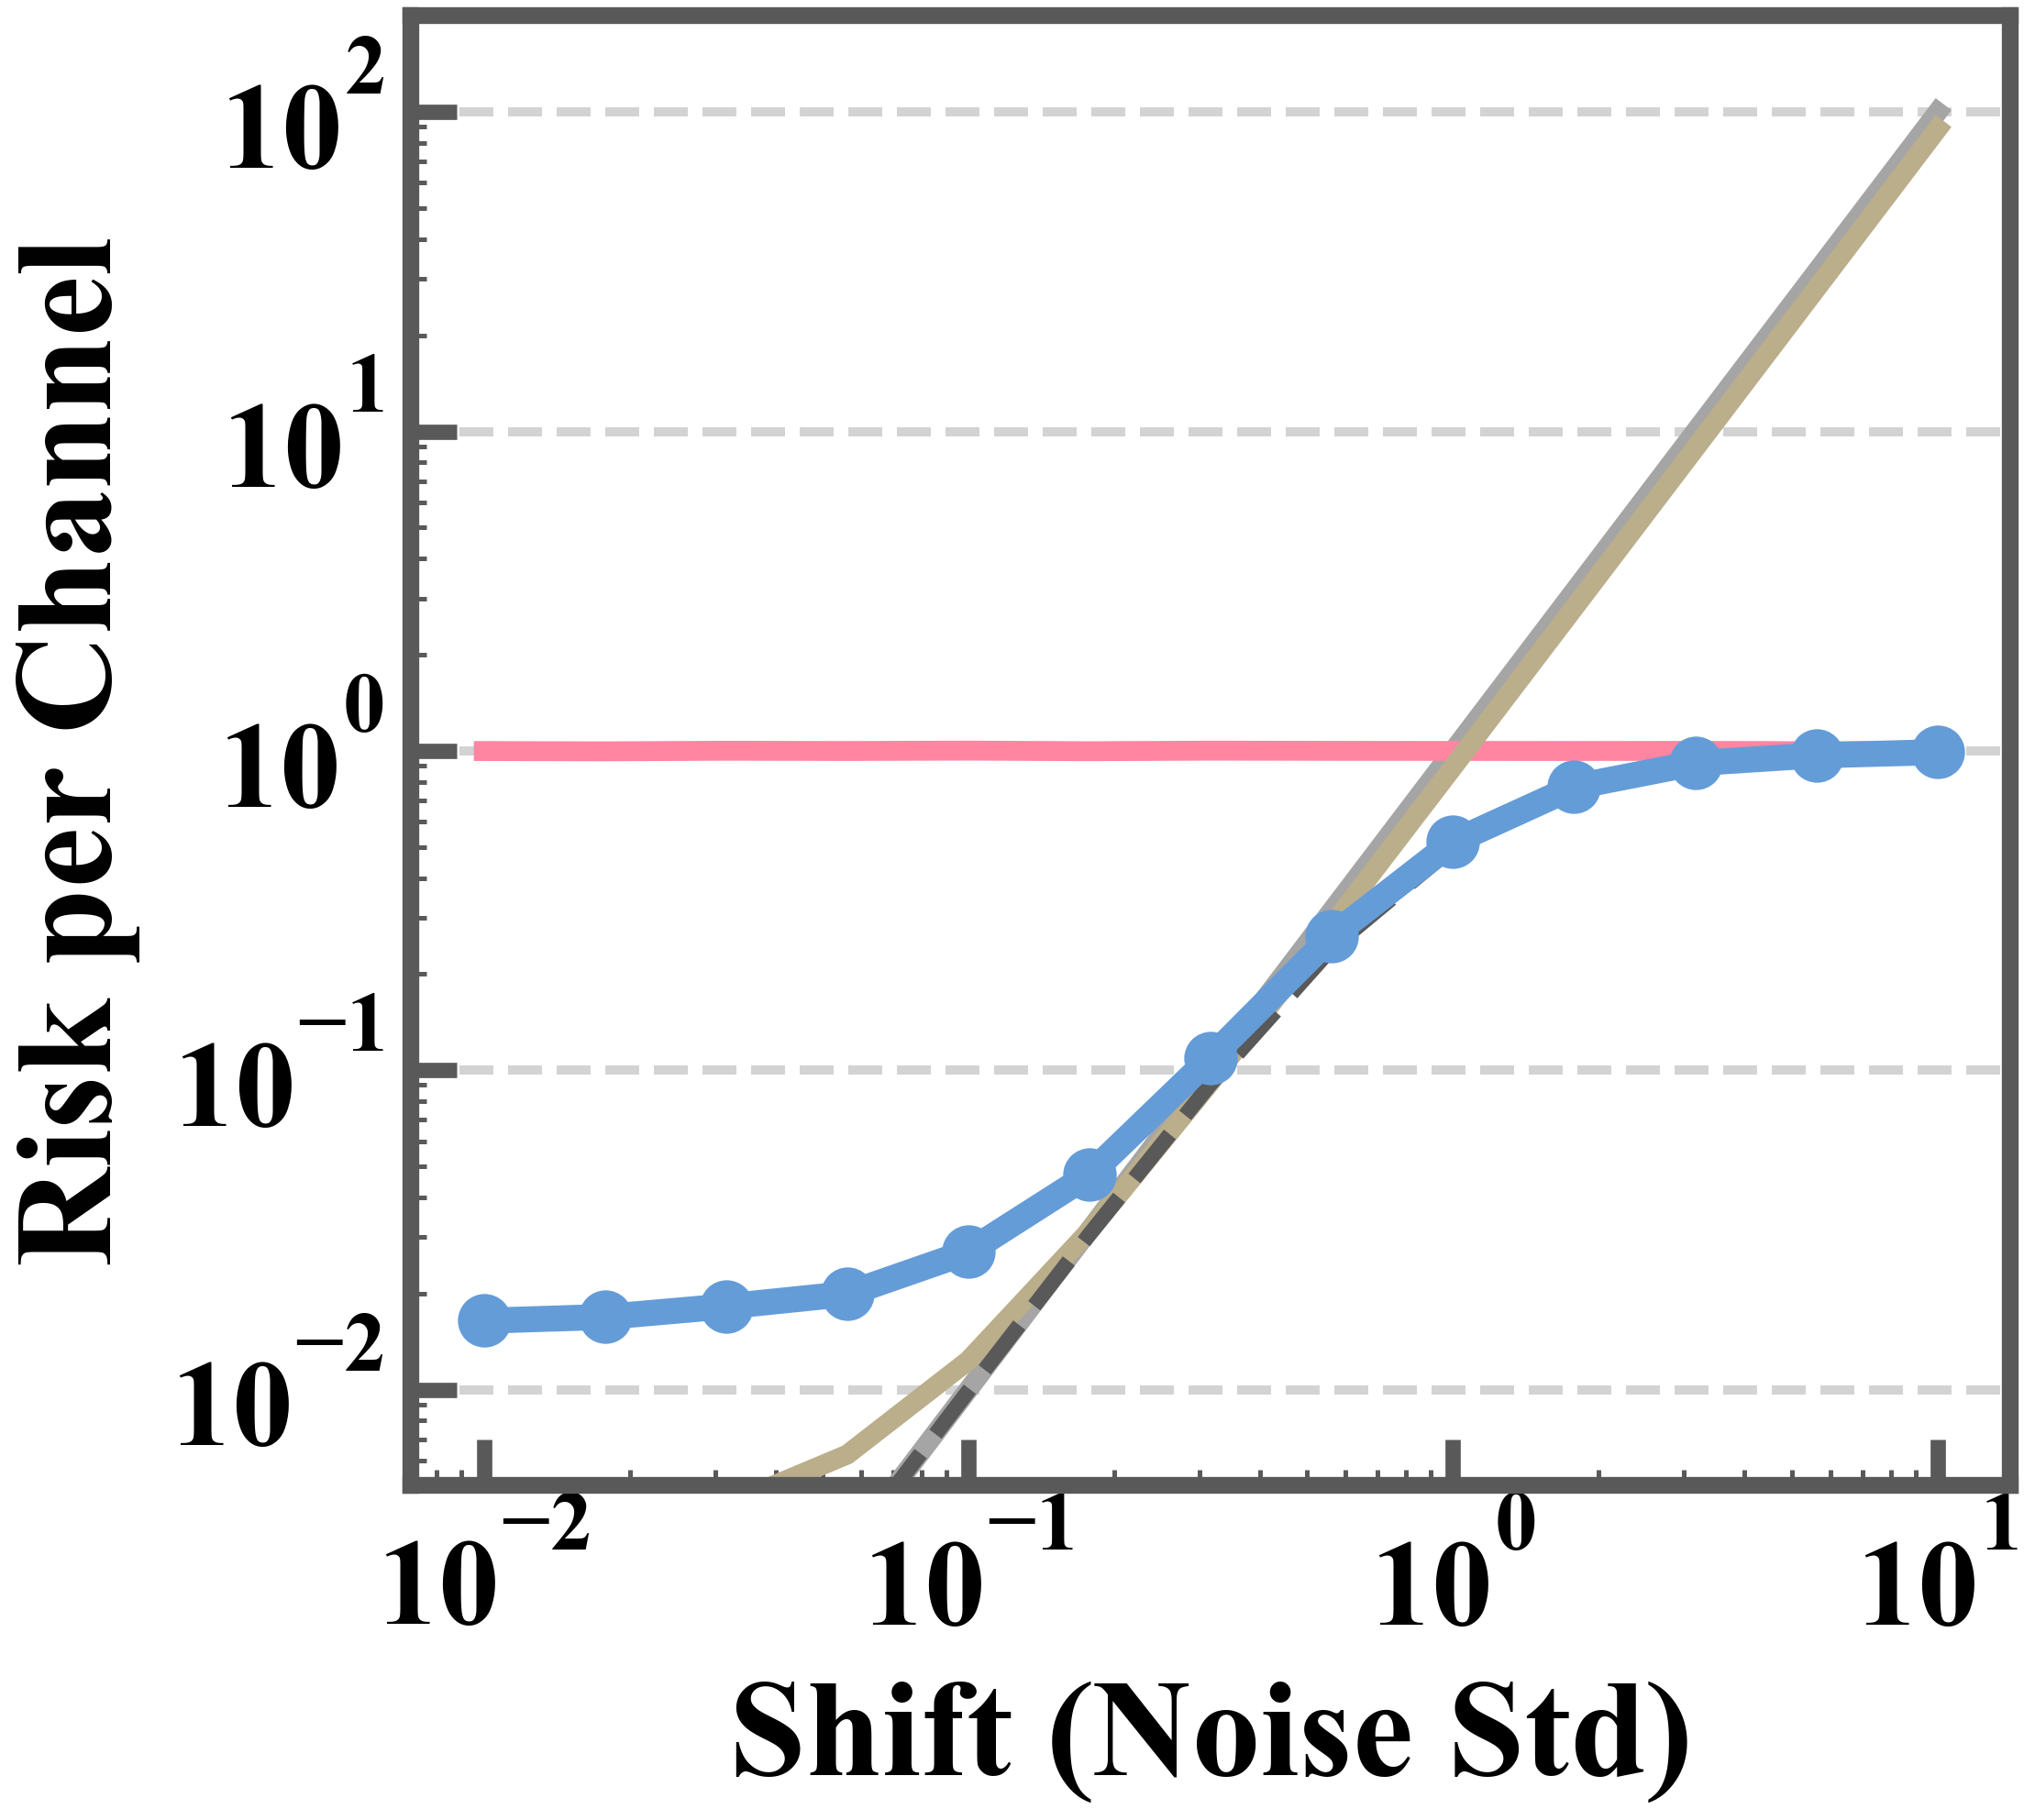
\includegraphics[width=\linewidth]{figures/exp/synthetic/risk_n1_gauss_s1p0.png}
        \caption{Gaussian, $n{=}1$.}
    \end{subfigure}\hfill
    \begin{subfigure}[t]{0.32\columnwidth}
        \centering
        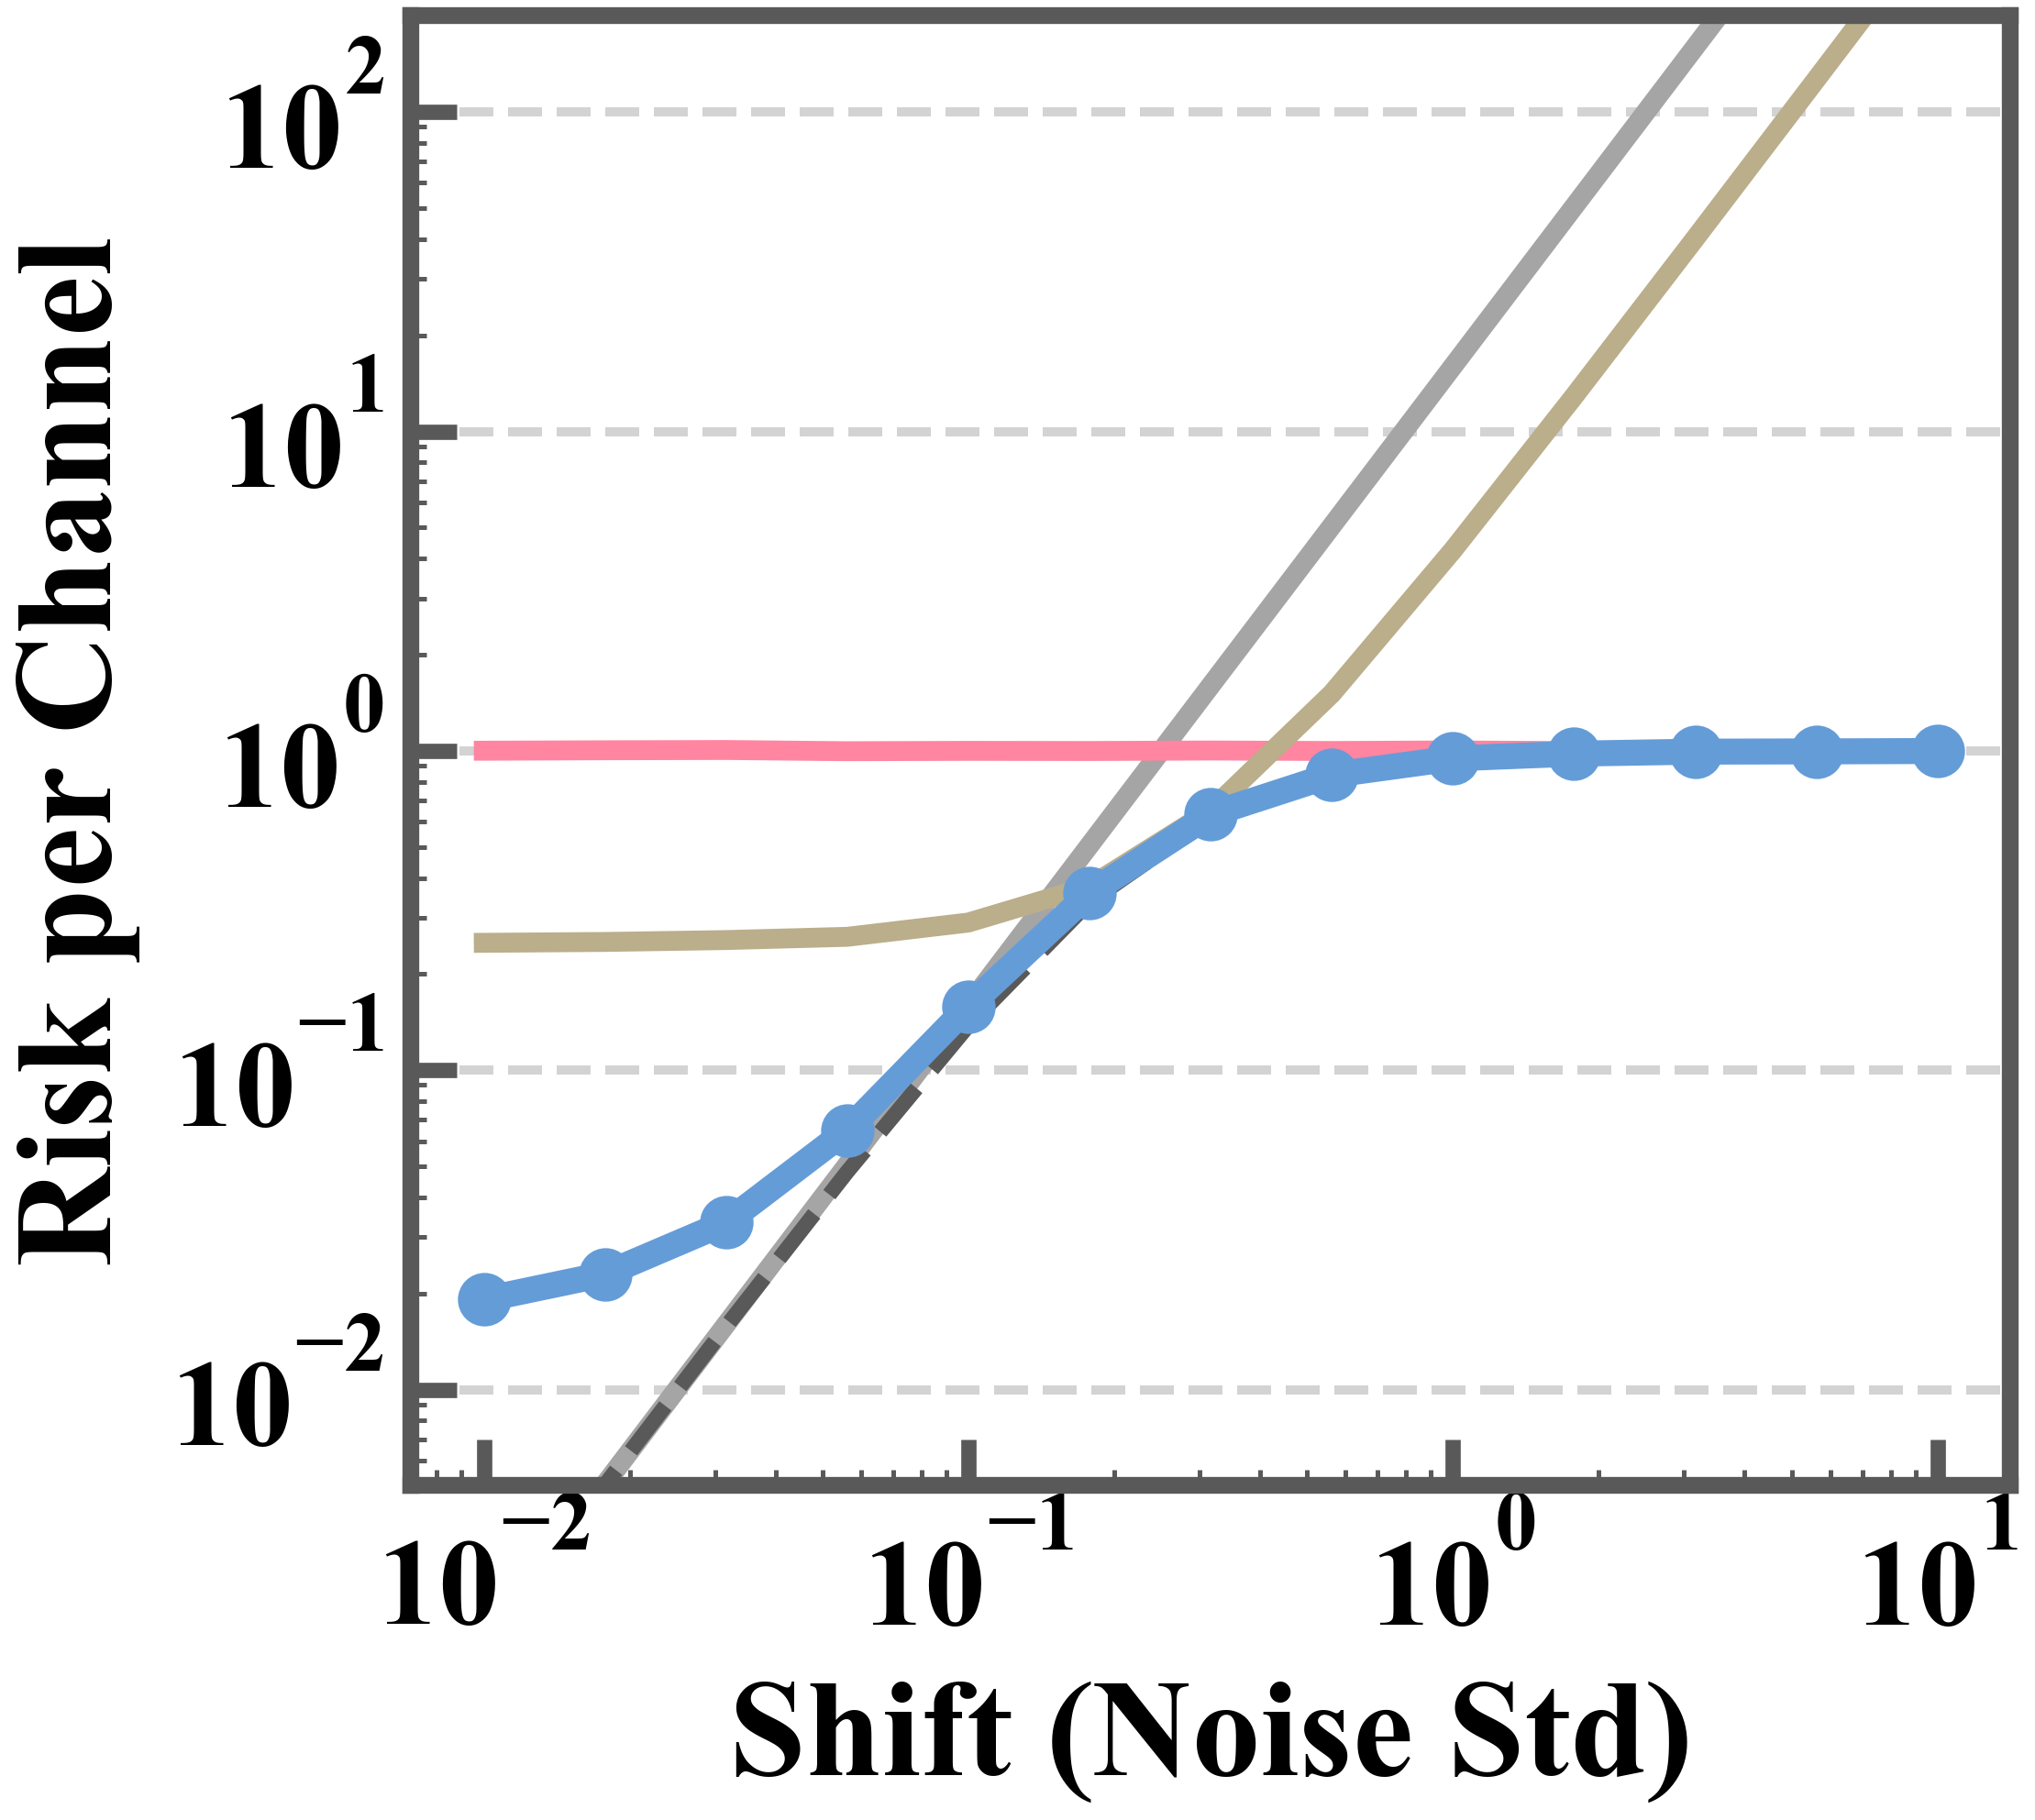
\includegraphics[width=\linewidth]{figures/exp/synthetic/risk_n16_gauss_s1p0.png}
        \caption{Gaussian, $n{=}16$.}
    \end{subfigure}\hfill
    \begin{subfigure}[t]{0.32\columnwidth}
        \centering
        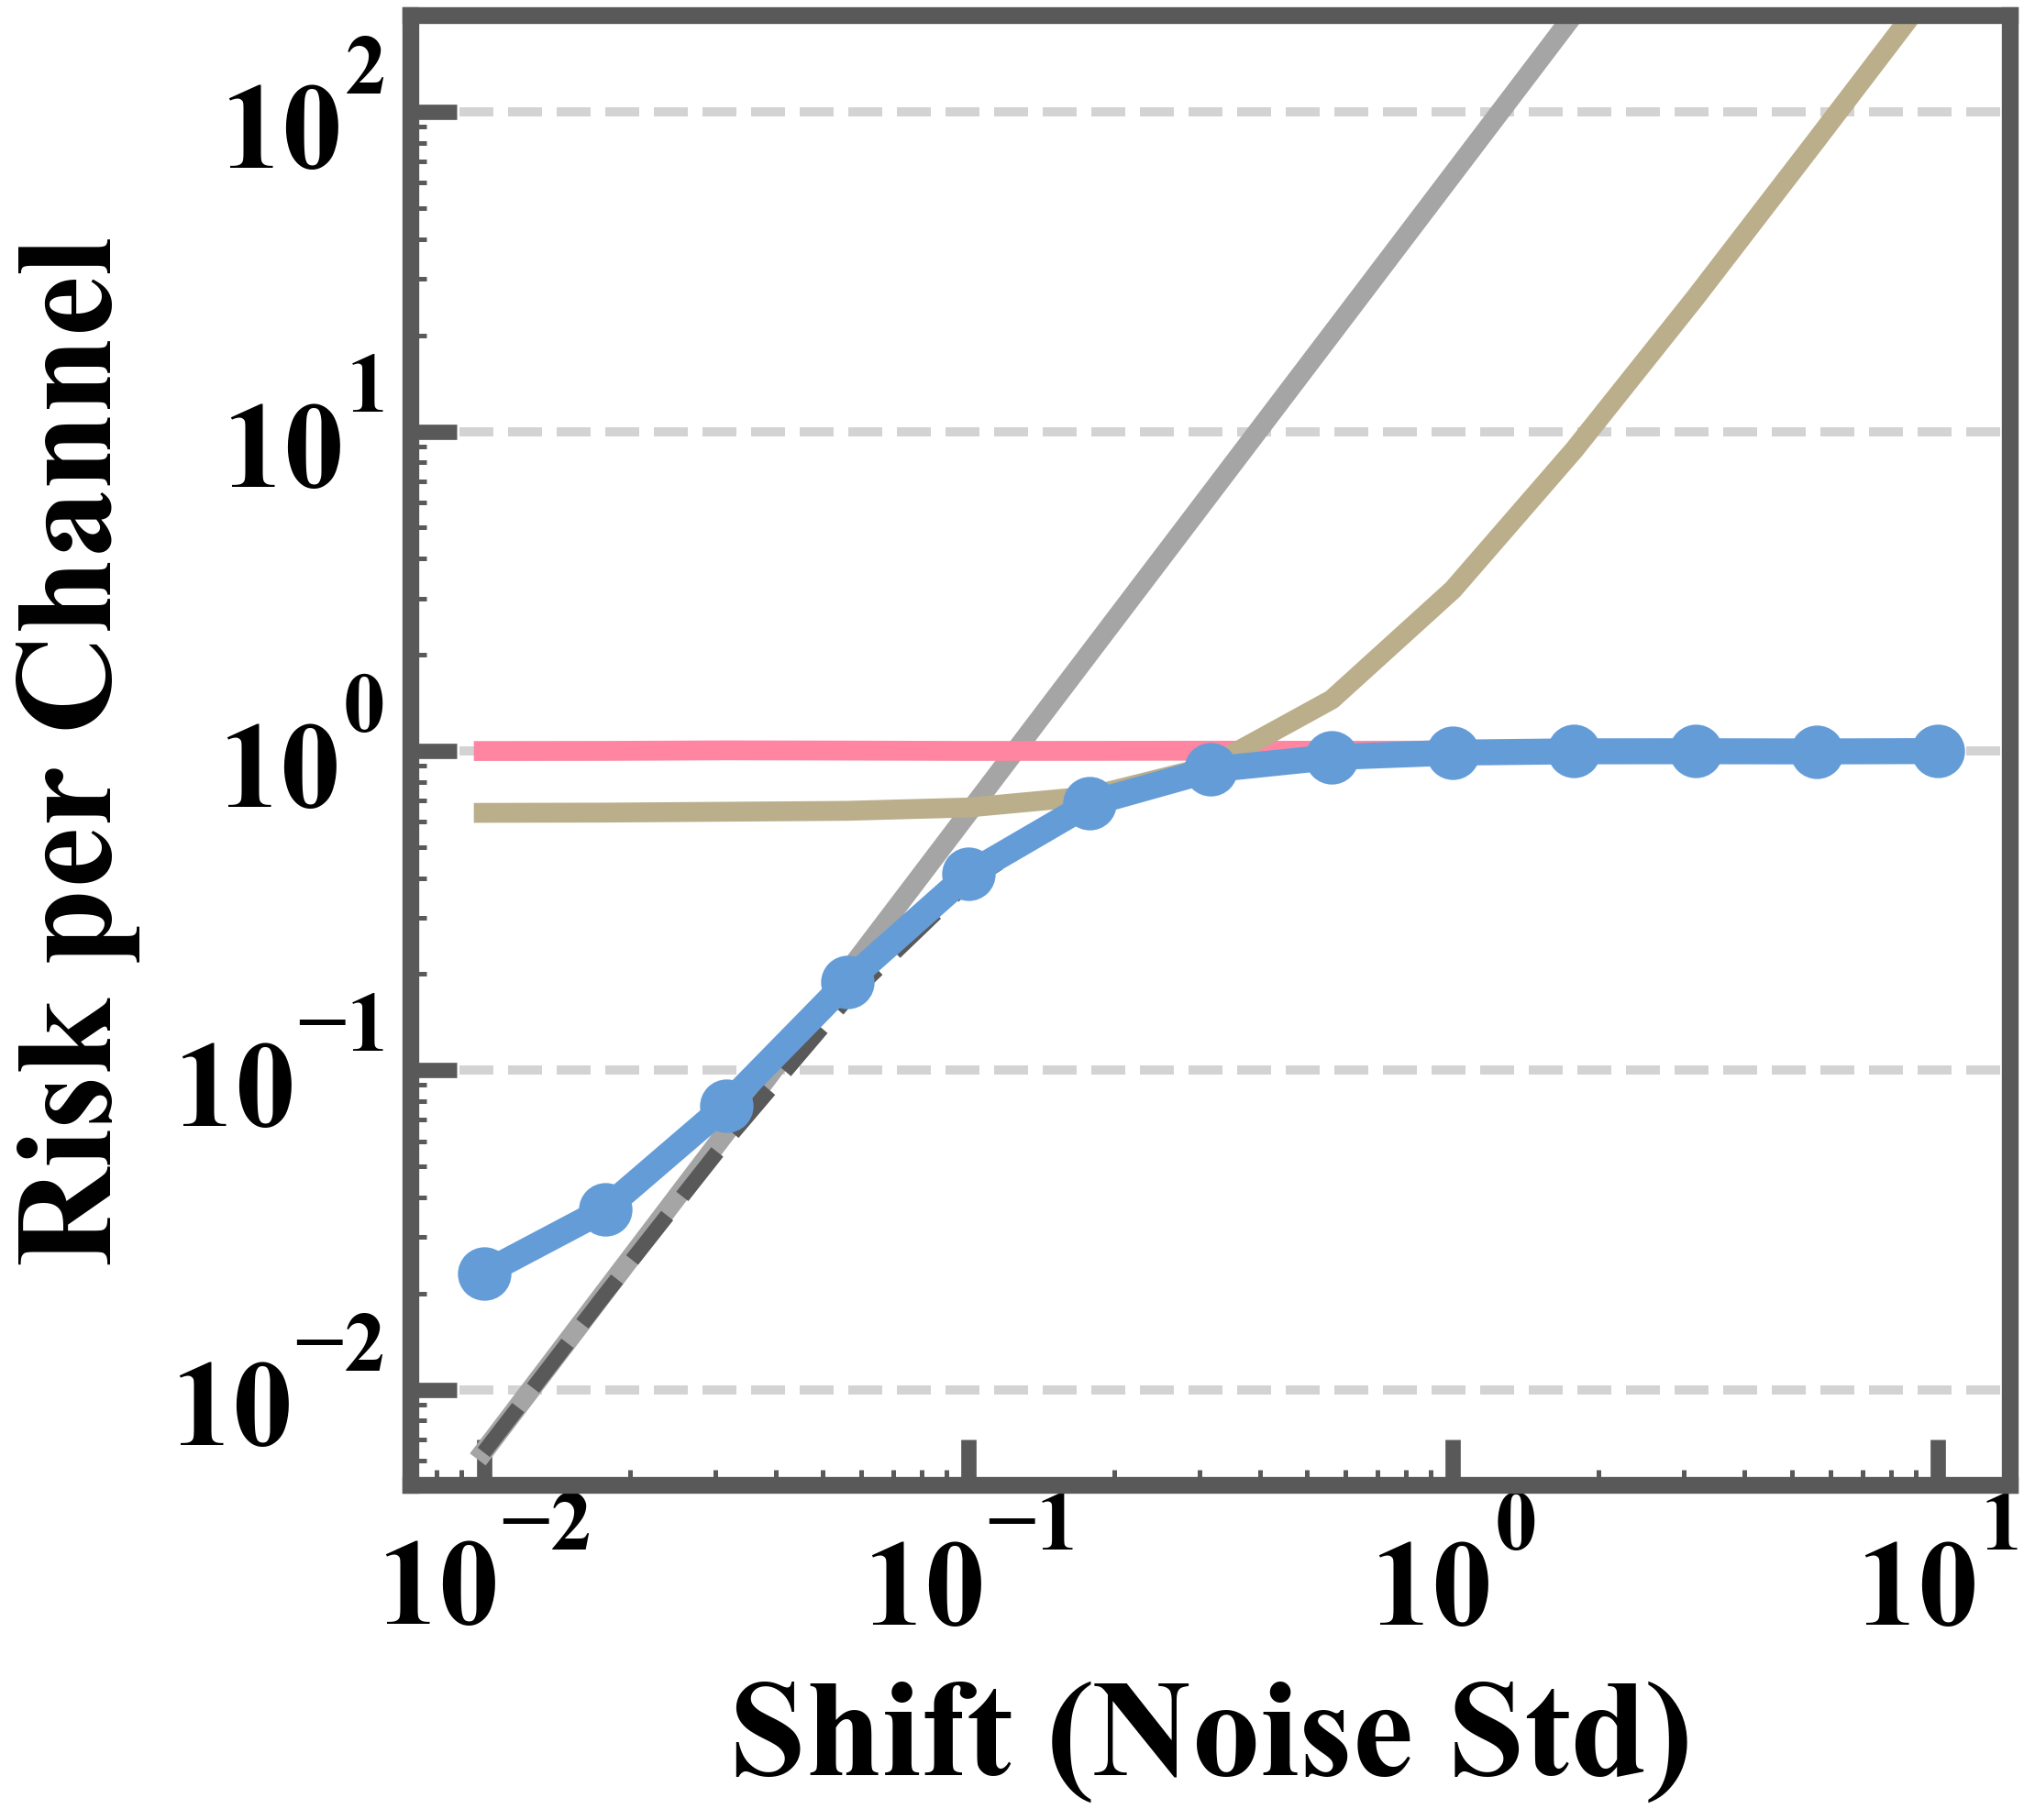
\includegraphics[width=\linewidth]{figures/exp/synthetic/risk_n64_gauss_s1p0.png}
        \caption{Gaussian, $n{=}64$.}
    \end{subfigure}
    \begin{subfigure}[t]{0.32\columnwidth}
        \centering
        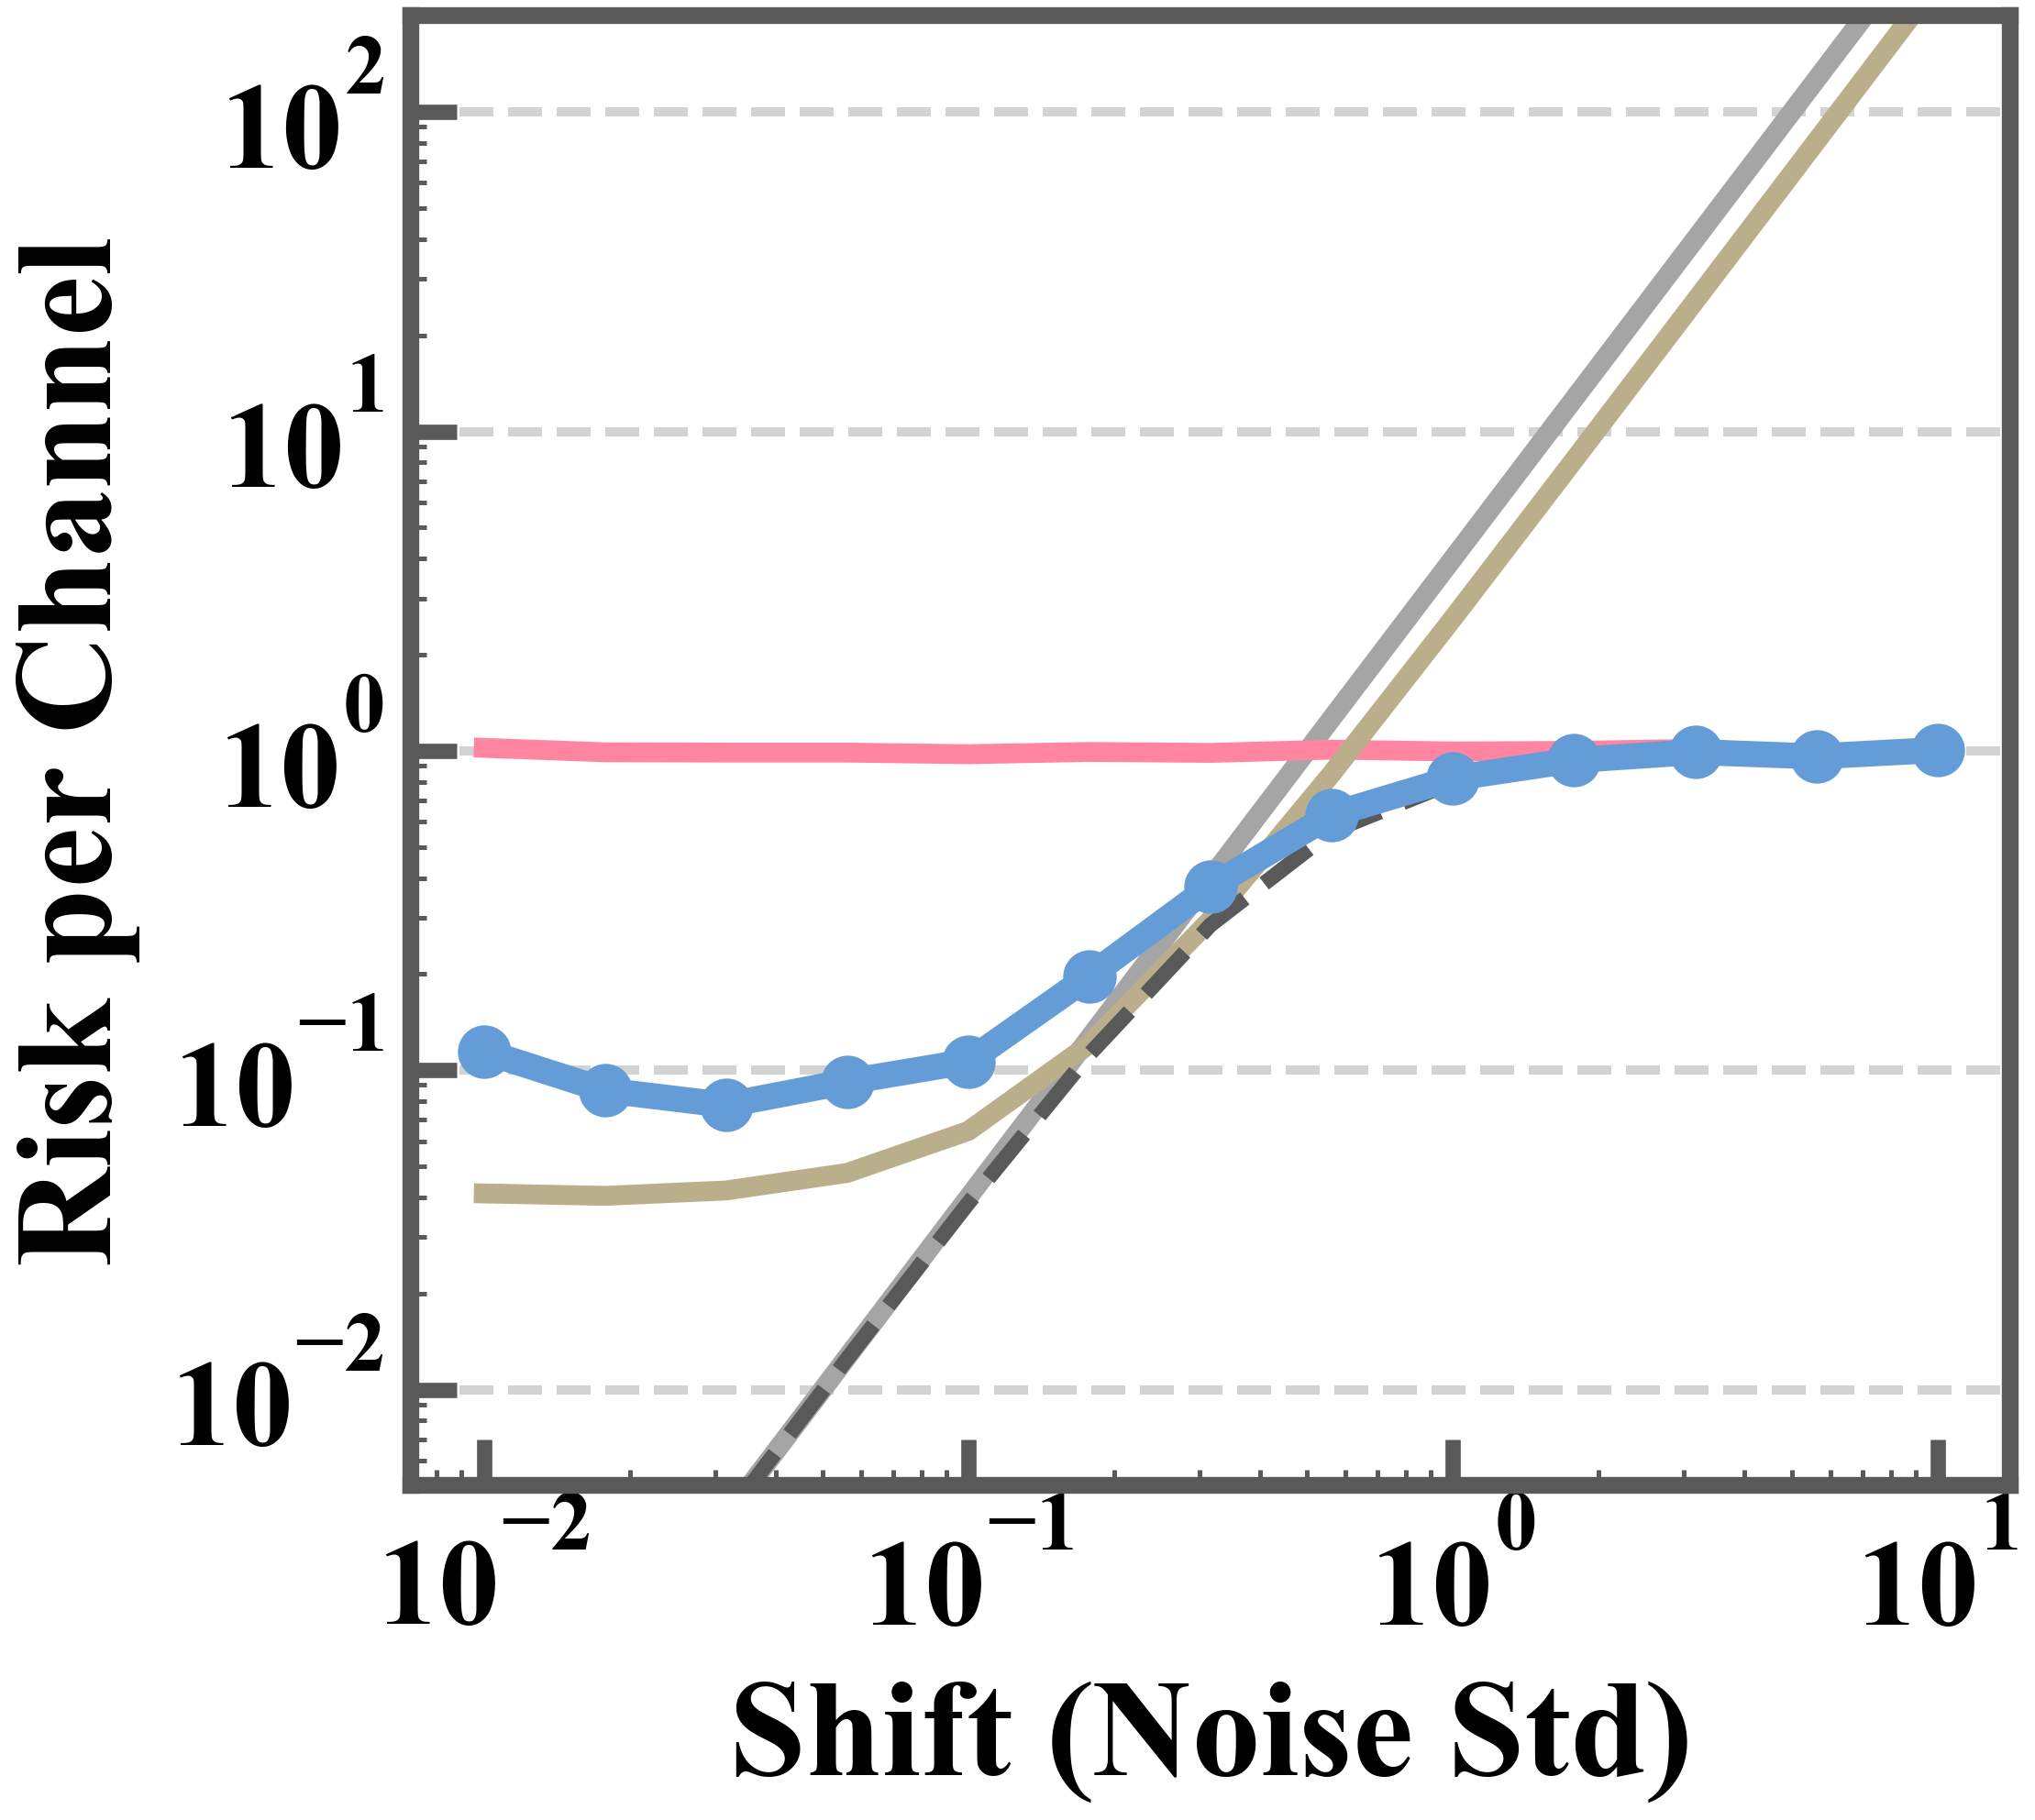
\includegraphics[width=\linewidth]{figures/exp/synthetic/risk_n4_student_t3_s1p0.png}
        \caption{Student-$t_3$, $n{=}4$.}
    \end{subfigure}\hfill
    \begin{subfigure}[t]{0.32\columnwidth}
        \centering
        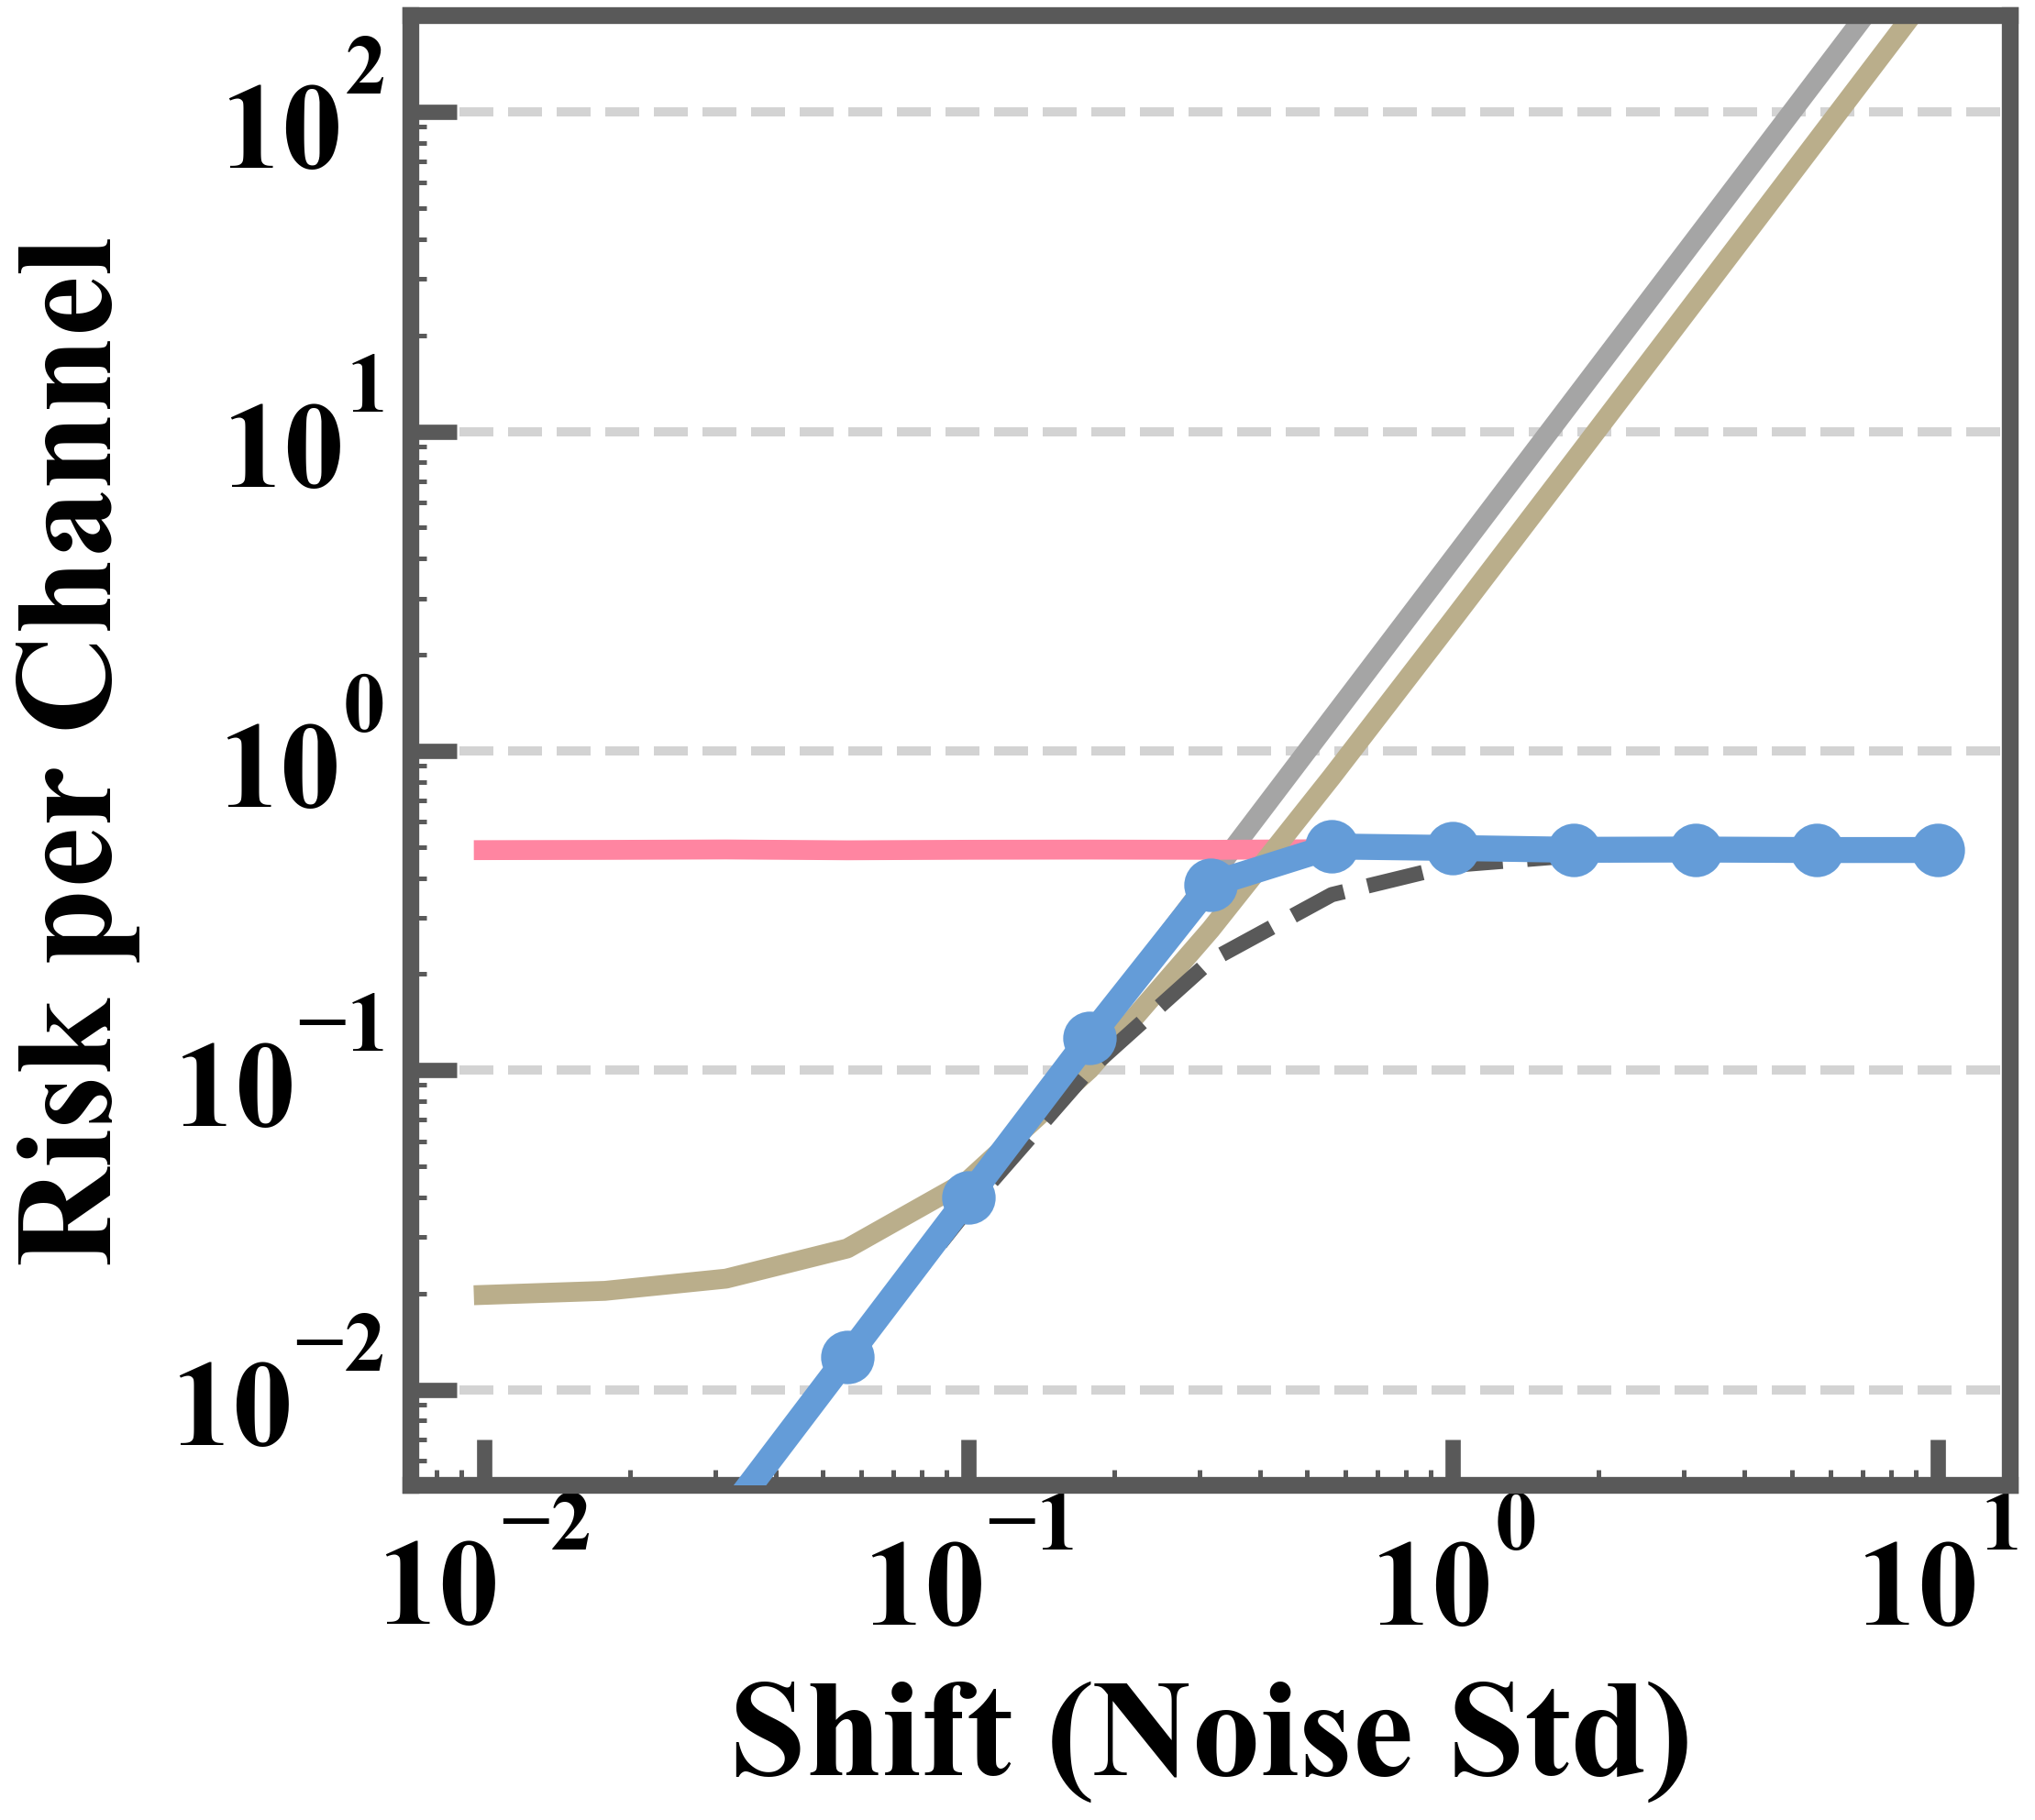
\includegraphics[width=\linewidth]{figures/exp/synthetic/risk_n4_gauss_s0p7.png}
        \caption{Noise $0.7\times$, $n{=}4$.}
    \end{subfigure}\hfill
    \begin{subfigure}[t]{0.32\columnwidth}
        \centering
        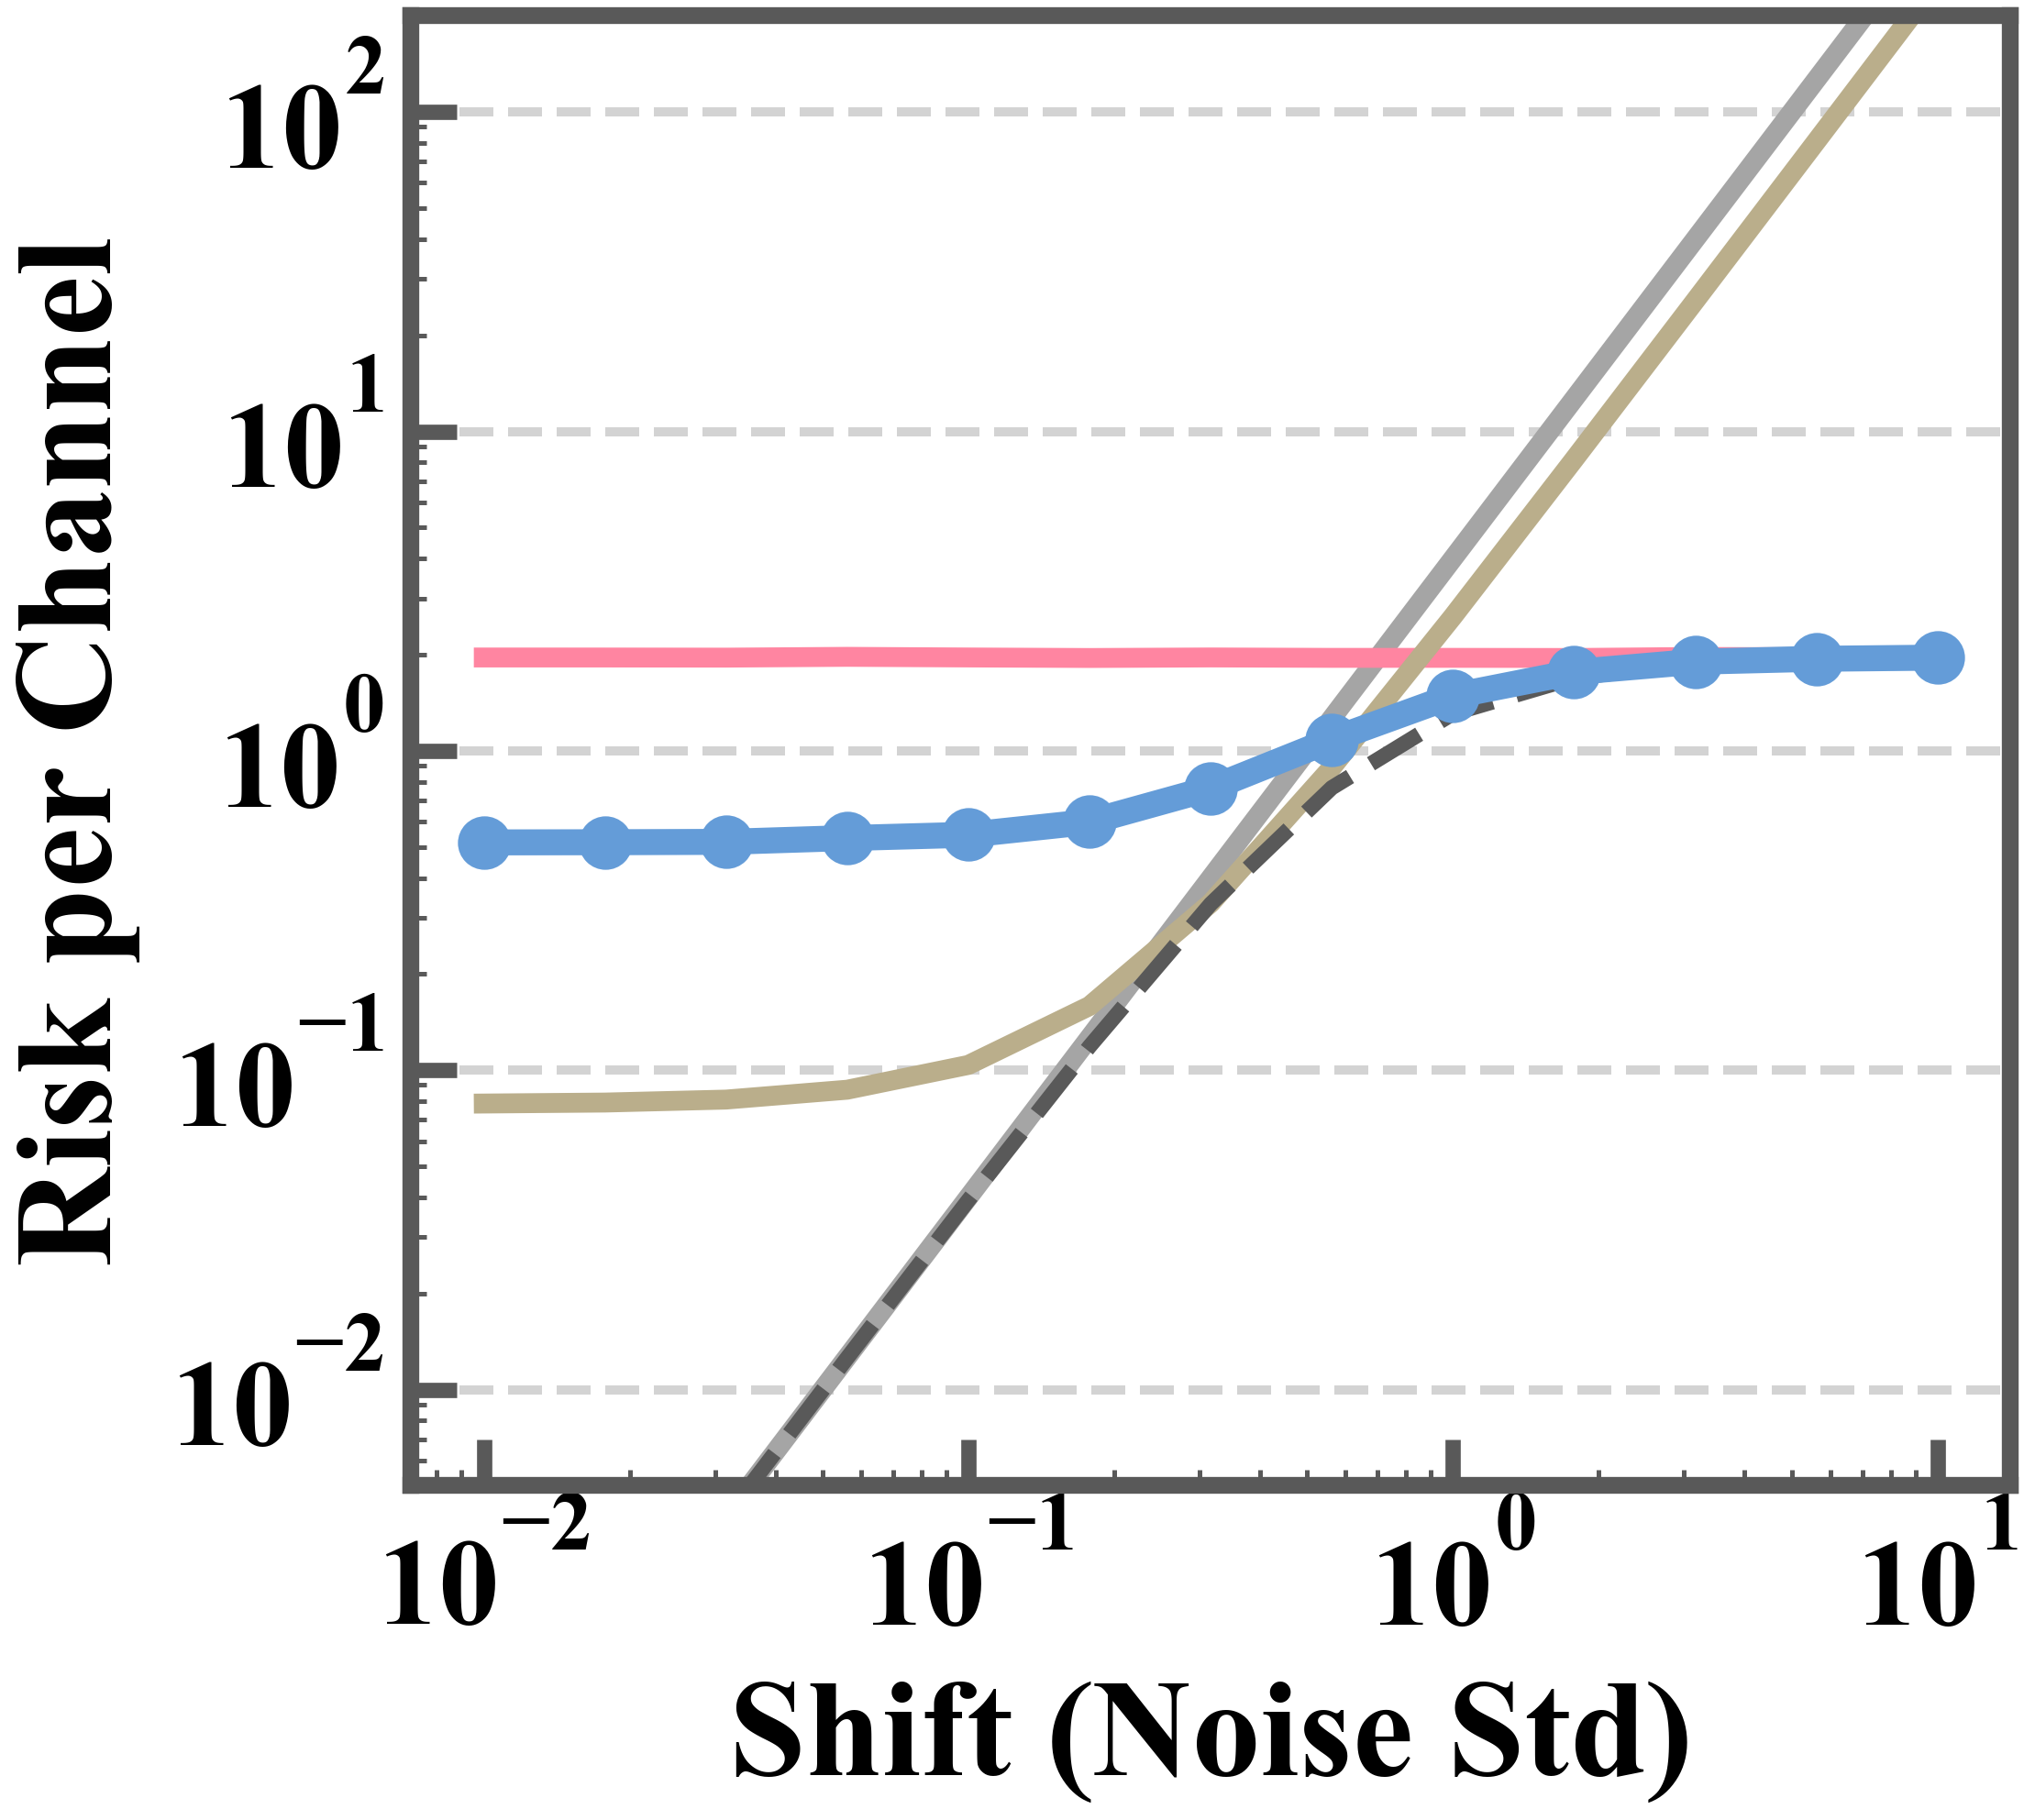
\includegraphics[width=\linewidth]{figures/exp/synthetic/risk_n4_gauss_s1p4.png}
        \caption{Noise $1.4\times$, $n{=}4$.}
    \end{subfigure}
    \caption{Risk per channel as a function of the per-channel shift in the simulation (log scales), with the legend of Figure~\ref{fig:teaser-figure}: Source (grey), TBN (pink), Prior-BN with $N{=}16$ (khaki), the oracle weight (dashed) and SourceStein (blue).}
    \label{fig:apdx-synthetic}
\end{figure}
           % A Related Works, then every appendix section
                                      % (one file named after its content,
                                      % latex_source.md section 11)

\end{document}
